\documentclass[12pt,a4paper]{article}
\usepackage[T1]{fontenc}\usepackage[utf8]{inputenc}
\usepackage{mathptmx}\usepackage[scaled=0.9]{helvet}\usepackage{courier}
\usepackage[margin=2.5cm]{geometry}
\usepackage{amsmath,amssymb,mathtools,bm}
\usepackage{booktabs,array,tabularx,longtable}
\usepackage{graphicx,xcolor,float}
\usepackage[font=small,labelfont=bf]{caption}
\usepackage{tikz}\usetikzlibrary{arrows.meta,positioning,shapes.geometric,fit,calc}
\usepackage[expansion=false]{microtype}
\usepackage{enumitem}\setlist{nosep,leftmargin=1.4em}
\usepackage[numbers,sort&compress]{natbib}
\usepackage[colorlinks=true,linkcolor=blue!50!black,citecolor=blue!50!black,urlcolor=blue!50!black]{hyperref}
\usepackage[nameinlink,capitalise]{cleveref}
\usepackage{fancyhdr}\pagestyle{fancy}\fancyhf{}\fancyhead[L]{\small\nouppercase{\leftmark}}\fancyfoot[C]{\thepage}\renewcommand{\headrulewidth}{0.3pt}
\setlength{\parskip}{0.45em}\setlength{\parindent}{0pt}\setlength{\headheight}{14pt}
\newcommand{\bu}{\bm u}\newcommand{\bq}{\bm q}\newcommand{\bx}{\bm x}\newcommand{\bn}{\bm n}
\DeclareMathOperator{\tr}{tr}\DeclareMathOperator{\Real}{Re}\DeclareMathOperator{\Imag}{Im}
\newcommand{\dd}{\mathrm d}\newcommand{\ii}{\mathrm i}
\title{\bfseries Waves in Thermoelastic and Multiphysics Continua:\\ Generalized Heat Conduction, Coupled Fields and Size Effects\\[2pt]\large A Unified Review with Verified Reductions, Dispersion Analysis and Benchmark Problems}
\author{Vipin Gupta\\{\small Gurugram University}\\{\small\texttt{vipin@gurugramuniversity.ac.in}}}
\date{\today}
\emergencystretch=3em
\begin{document}
\maketitle
\begin{abstract}
Wave propagation in solids that conduct heat, deform, and carry further fields such as electric polarization, magnetic induction, diffusing species or microstructural degrees of freedom is governed by a family of coupled models that is usually presented one member at a time. This review organises that family around a single heat-flux template with three lags and one memory term, shows how the classical, Lord--Shulman, Green--Lindsay, Green--Naghdi, dual-phase-lag, three-phase-lag, Moore--Gibson--Thompson, fractional and memory-dependent theories arise (or fail to arise) as parameter choices, and records exactly which limits are regular and which are singular, including a correction to a widely repeated stability statement for the dual-phase-lag model. For the coupled problem we derive and symbolically verify a single dispersion polynomial, and use it to compare phase speed, attenuation and thermoelastic damping across theories; we then treat transient problems (heat pulse, thermal shock), Rayleigh waves, reflection and interface energy partition, piezoelectric, magneto-thermoelastic, diffusive and microstructural couplings, and nonlocal and gradient size effects against lattice dispersion. We discuss analytical and numerical solution techniques with a benchmark, applications from laser ultrasonics to micro-resonators and tissue heating, and close with a comparative synthesis, a pitfalls checklist, a decision guide and a research agenda. We also provide flexural and plate thermoelastic damping validated against exact solutions, anisotropic and free-surface reflection results, a finite-difference benchmark for hyperbolic heat conduction, worked examples and reporting standards. All quantitative figures are generated by accompanying scripts and the key identities are checked symbolically or numerically.
\medskip

\noindent\textbf{Keywords:} generalized thermoelasticity; second sound; dual-phase-lag; Moore--Gibson--Thompson; fractional heat conduction; memory-dependent derivative; nonlocal elasticity; piezoelectricity; Rayleigh waves; thermoelastic damping; interface energy partition.
\end{abstract}
\tableofcontents
\newpage
\section{Introduction}\label{sec:intro}
\subsection{The problem that generalized thermoelasticity addresses}
Heat conduction in solids is described, to an excellent approximation under ordinary conditions, by Fourier's law: the heat flux is proportional to the temperature gradient at the same instant. Combined with energy balance this gives a parabolic equation, whose solutions have a property that is physically uncomfortable: a temperature disturbance applied at one point changes the temperature everywhere else at the same instant, however small the change may be. For slow processes in bulk matter the discrepancy between this instantaneous response and what a real, finite-speed carrier of heat would do is immeasurably small. It becomes measurable, and sometimes dominant, when the heating or loading is very fast (femtosecond to nanosecond laser pulses), when the structure is very small or very cold so that phonon mean free paths approach the structure size, when the medium is strongly heterogeneous, or when the observed quantity is a high-frequency elastic wave whose period is comparable to a thermal relaxation time.

Thermoelasticity couples this thermal field to deformation: heating produces thermal stress through thermal expansion, and deformation changes the temperature through the dilatation term in the energy balance. The classical coupled theory of Biot \citep{Biot1956}, building on the thermomechanical stress--strain law of Duhamel and Neumann \citep{Duhamel1837} and the early dynamic solutions of Danilovskaya \citep{Danilovskaya1950} and Chadwick and Sneddon \citep{ChadwickSneddon1958,Chadwick1960}, inherits the infinite thermal signal speed. The extensions that remove it, collectively called \emph{generalized} or \emph{non-classical} thermoelasticity \citep{Chandrasekharaiah1986,Chandrasekharaiah1998,HetnarskiIgnaczak1999,HetnarskiIgnaczak2000,IgnaczakOstoja2010}, now form one of the largest strands of continuum mechanics, with a very large body of theoretical work. At the same time two further developments widened the field. First, devices exploit the coupling of deformation and temperature to additional physical fields, above all electric polarization (piezoelectricity and pyroelectricity), but also magnetic induction, diffusing species, fluid-filled pores and microstructural kinematics \citep{Mindlin1974Thermopiezo,Nowacki1978,Eringen1999,Iesan2004}. Second, at small scales the local stress--strain relation itself fails to describe dispersion, and nonlocal and gradient enrichments are used \citep{Eringen1972,Eringen1983,Aifantis1992,Askes2011}.

\subsection{Why another review}
Reviews of generalized thermoelasticity exist and are excellent \citep{Chandrasekharaiah1986,Chandrasekharaiah1998,HetnarskiIgnaczak1999,HetnarskiIgnaczak2000,Shakeriaski2021,Huang2025}. What has been lacking is a treatment that serves a reader who wants to \emph{use} the theories for wave problems and compare them reliably. Three observations motivate the present organisation.
\begin{enumerate}
\item \textbf{Proliferation without a common language.} Over the past three decades the number of named heat-conduction models for thermoelastic waves has grown very large, many of them combinations (two-temperature fractional Lord--Shulman, three-phase-lag with memory, nonlocal Moore--Gibson--Thompson, and so on). Each paper introduces its own constants and notation. Section~\ref{sec:framework-link} introduces a single heat-flux function $G(s)$ in the Laplace domain through which every linear model passes, so that a new combination is understood as a new choice of $G$.
\item \textbf{Unreliable folklore about limits and stability.} Several statements are repeated across papers without re-derivation: which parameter limits reduce one model to another, which parameter ranges are stable, how the wave branches should be labelled. We re-derive these and check them numerically. One widely repeated statement---that dual-phase-lag thermoelasticity requires $\tau_T\ge\tau_q/2$ to be stable---turns out to depend on the order of the Taylor expansion that defines the model (Section~\ref{sec:lags}).
\item \textbf{Figures that cannot be compared.} Published dispersion and response curves use different nondimensionalisations, parameter sets and branch conventions, so that the visual impression of ``the effect of the fractional order'' or ``the effect of nonlocality'' is hard to calibrate. We use one nondimensionalisation throughout, quantified by a small number of material-independent groups.
\end{enumerate}

\subsection{Contributions and organisation}
This review does not report new experiments. Its contributions are:
\begin{itemize}
\item a unified heat-flux template, a table of \emph{exact} reductions and singular limits, and a taxonomy that places the main models in relation to one another (Sections~\ref{sec:framework-link}--\ref{sec:memory});
\item a coupled dispersion polynomial valid for the whole template, verified symbolically, and comparative dispersion, damping and speed results (Sections~\ref{sec:classical}--\ref{sec:waves3d});
\item benchmark transient problems, namely the heat pulse and the thermal shock of a half-space, each with a Laplace-domain closed form and a numerical inversion (Section~\ref{sec:transient});
\item thermoelastic Rayleigh waves, reflection and interface energy partition, with limit checks (Sections~\ref{sec:surface}--\ref{sec:interfaces});
\item a treatment of size effects contrasted with lattice dispersion, and of the principal multiphysics couplings (Sections~\ref{sec:size}--\ref{sec:multi});
\item a kinetic basis for the Cattaneo and Guyer--Krumhansl laws with the dispersion of the latter (\cref{sec:kinetic}), and a quantitative test of how well Taylor-truncated lag laws represent the delay law they approximate (\cref{sec:delayfid});
\item flexural thermoelastic damping, including a plate (Lamb-wave) computation validated against the Rayleigh--Lamb equation and the Lifshitz--Roukes solution, resonant modes of a bar, anisotropy in cubic crystals, free-surface reflection and piezoelectric surface waves (\cref{sec:flexted,sec:aniso,sec:reflection,sec:lamb,sec:bar,sec:bg});
\item a discussion of solution methods with finite-difference and inversion benchmarks, experimental evidence and parameter identification, worked examples, application regimes, reporting standards, a comparative synthesis with a pitfalls checklist and a decision guide, and a research agenda (\cref{sec:methods,sec:schemes,sec:applications,sec:scenarios,sec:examples,sec:experiments,sec:synthesis,sec:reporting,sec:open}).
\end{itemize}
Section~\ref{sec:history} gives the historical and literature background. Section~\ref{sec:foundations} derives the thermomechanical foundations that the remaining sections rely on. Readers primarily interested in choosing a model can go directly to Section~\ref{sec:synthesis}.

\subsection{Scope and conventions}\label{sec:conventions}
We treat \emph{linear} wave propagation in homogeneous solids about a uniform reference state at temperature $T_0$ unless stated otherwise; nonlinear thermoelasticity, large deformation, radiative transport and chemically reacting media are outside our scope. The following notation is used throughout.

\begin{table}[ht]\centering\small
\caption{Principal notation. Indices follow the Einstein summation convention; a comma denotes a spatial derivative and a dot a time derivative.}\label{tab:notation}
\begin{tabular}{@{}lp{4.1cm}lp{4.3cm}@{}}\toprule
$u_i,\ \varepsilon_{ij}$ & displacement, strain & $\sigma_{ij}$ & stress\\
$\theta=T-T_0$ & temperature increment & $T_0$ & reference temperature\\
$q_i$ & heat flux & $v$ & thermal displacement, $\dot v=\theta$\\
$\rho$ & mass density & $c$ & specific heat at constant strain\\
$\lambda,\mu$ & Lam\'e constants & $\alpha_T$ & linear expansion coefficient\\
$\beta=(3\lambda+2\mu)\alpha_T$ & thermal-stress coefficient & $k,\ k^*$ & conductivities (Fourier, GN)\\
$\tau_q,\tau_T,\tau_v$ & relaxation time and lags & $\alpha=k/\rho c$ & thermal diffusivity\\
$c_1=\sqrt{(\lambda+2\mu)/\rho}$ & isothermal P-wave speed & $c_2=\sqrt{\mu/\rho}$ & shear wave speed\\
$\varepsilon=\beta^2T_0/(\rho^2cc_1^2)$ & thermoelastic coupling & $\omega_*=\rho c c_1^2/k$ & thermal characteristic frequency\\
$G(s)$ & heat-flux function (Eq.~\eqref{eq:G}) & $s=-\ii\omega$ & Laplace variable / complex frequency\\
$c_T$ & thermal wave speed & $K^2$ & electromechanical coupling\\
$\xi,\ \ell$ & nonlocal and gradient lengths & $Z=\rho c$ & mechanical impedance\\
\bottomrule\end{tabular}
\end{table}
The strain tensor is always written with two indices ($\varepsilon_{ij}$) so that it is not confused with the scalar coupling $\varepsilon$. Plane waves are $\exp[\ii(kx-\omega t)]$ with $\Imag k\ge0$ for spatial decay in the propagation direction, and a ``branch'' of the dispersion relation is a root $k(\omega)$ followed by continuity in $\omega$.

\subsection{Reproducibility}
All figures in this review that display numerical results were produced by Python scripts that accompany the manuscript, and the identities used repeatedly (the coupled dispersion polynomial, the Debye form of weak-coupling damping, the Green--Naghdi type-II wave speeds, the reductions of Table~\ref{tab:param}) are checked either symbolically or against independent numerical roots in those scripts (Appendix~\ref{app:repro}). Where a quantity depends on a choice of model variant, for example the form of a memory-dependent derivative, the choice is stated next to the result.

\begin{summarybox}[Summary]
This review organises the generalized thermoelasticity literature around one heat-flux template with three lags and one memory term, derives a single dispersion polynomial checked symbolically against the field equations, and provides verified benchmarks. Scope: linear waves about a uniform reference state, isotropic and anisotropic solids, plane-wave and guided-wave problems. Contributions: correction to the DPL stability condition, GN-III front-speed clarification, net-flux-vs-mode-flux check at interfaces, reporting standards. Not covered: nonlinear effects, radiative/reactive heat transfer, full bounded-domain well-posedness literature.
\end{summarybox}

\section{Historical development and the literature landscape}\label{sec:history}
\subsection{A short history}
\paragraph{Origins (1830s--1950s).} Duhamel's memoir of 1837 \citep{Duhamel1837} established the stress--strain--temperature relation that still bears his name (with Neumann's later contribution): the stress depends on strain and on the temperature increment through an expansion coefficient. The dynamic coupling appeared much later. Biot \citep{Biot1956} showed that the classical thermoelastic equations follow from the thermodynamics of irreversible processes with a Rayleigh-type dissipation function, and Danilovskaya \citep{Danilovskaya1950} solved the thermal shock of an elastic half-space, in the uncoupled approximation. Chadwick and Sneddon \citep{ChadwickSneddon1958} analysed plane waves in the coupled theory; Chadwick's chapter \citep{Chadwick1960} became the standard reference for the dynamical theory; compact textbook accounts followed \citep{Boley1960,Nowacki1975,Carlson1972}. The core results of that period are that the coupled longitudinal wave is attenuated and dispersed, that shear waves decouple in isotropic media, and that the thermal disturbance is a diffusive wave. Zener's earlier analysis of thermoelastic internal friction in vibrating reeds \citep{Zener1937} had already shown the same relaxation behaviour from a different direction.

\paragraph{Finite-speed heat conduction (1940s--1970s).} The conceptual starting point is Cattaneo's 1948 note \citep{Cattaneo1948} and Vernotte's independent discussion \citep{Vernotte1958}, which add a relaxation term to Fourier's law, making the heat equation hyperbolic. Experimental support from low-temperature solids, namely second sound in solid helium and in sodium fluoride \citep{Ackerman1966,Jackson1970}, and a kinetic theory of phonon hydrodynamics \citep{GuyerKrumhansl1966,GuyerKrumhansl1966II,Chester1963}, supplied physical contexts in which heat actually propagates as a wave. Lord and Shulman \citep{Lord1967} then built Cattaneo's law into a complete thermoelastic theory, and Green and Lindsay \citep{Green1972} proposed a different extension with two relaxation times in the constitutive relations. The relation between these theories and thermodynamics was the subject of extensive discussion; reviews are \citep{Chandrasekharaiah1986,Joseph1989,Joseph1990}.

\paragraph{Energy-based theories (1990s).} Green and Naghdi \citep{Green1991,GreenGN1992,Green1993} introduced a family of three theories (types I, II, III) based on an entropy balance rather than an entropy inequality for the heat flux, in which the thermal displacement plays the role of a potential. Type II is a nondissipative theory with undamped thermal waves; type III contains classical damping and thermal waves. Uniqueness and stability theory developed around these \citep{Chandrasekharaiah1996}.

\paragraph{Lagging models (1995--2010).} Tzou \citep{Tzou1995,Tzou1997} proposed that the heat flux and the temperature gradient are separated by delay times, giving the dual-phase-lag (DPL) model; Roy Choudhuri \citep{RoyChoudhuri2007} added a third lag associated with the thermal displacement. These models quickly spread because Taylor expansion of the lag equation gives a differential equation of finite order whose parameters can be chosen to fit data, and the stability and thermodynamic admissibility of those truncations has been studied extensively \citep{Quintanilla2003DPL,Chirita2016,Tibullo2017,vanDerMerwe2021}.

\paragraph{Nonlocal, fractional and memory-dependent extensions (1970s--present).} Eringen's nonlocal elasticity \citep{Eringen1972,Eringen1983,Eringen2002} and its thermoelastic extension \citep{Eringen1974} predate the generalized heat theories but converge with them in micro- and nanosystems; gradient elasticity \citep{Aifantis1992,Aifantis2003,Askes2006,Askes2011} is the other main enrichment. Fractional calculus entered heat conduction through the Caputo derivative \citep{Caputo1967}, was developed into fractional thermoelasticity \citep{Povstenko2004,Povstenko2007,Povstenko2009,Povstenko2011Cattaneo,Povstenko2016,Sherief2010Fractional,Ezzat2011}, and was joined by the memory-dependent derivative of Wang and Li \citep{Wang2011,Wang2021}. Two-temperature theories \citep{ChenGurtin1968,Youssef2006} and their hyperbolic variants \citep{Prasad2020,Alzahrani2020,Bassiouny2020} introduced a distinction between conductive and thermodynamic temperature.

\paragraph{Mathematical thermoelasticity of third order (2010s).} The Moore--Gibson--Thompson (MGT) equation, which arose in nonlinear acoustics \citep{MooreGibson1960}, was studied systematically as an evolution problem \citep{MarchandMcDevittTriggiani2012,LasieckaWang2015MGT,DellOroLasieckaPata2016MGT,DellOroPata2016Viscoelasticity} and then brought into thermoelasticity by Quintanilla \citep{Quintanilla2019,Bazarra2021MGTradial}, producing a model that fits the template of Section~\ref{sec:framework-link}.

\paragraph{Multiphysics and structure (1960s--present).} Micropolar and microcontinuum theories \citep{Eringen1966a,TauchertClausAriman1968,Eringen1999}, materials with voids \citep{Nunziato1979,Cowin1983,Iesan1986}, thermopiezoelectricity \citep{Mindlin1974Thermopiezo,Nowacki1978,Chandrasekharaiah1984}, and thermoelastic diffusion and magneto-thermoelasticity extended the mechanical content, usually with the heat law as an independent module.

\begin{figure}[t]\centering
\resizebox{\linewidth}{!}{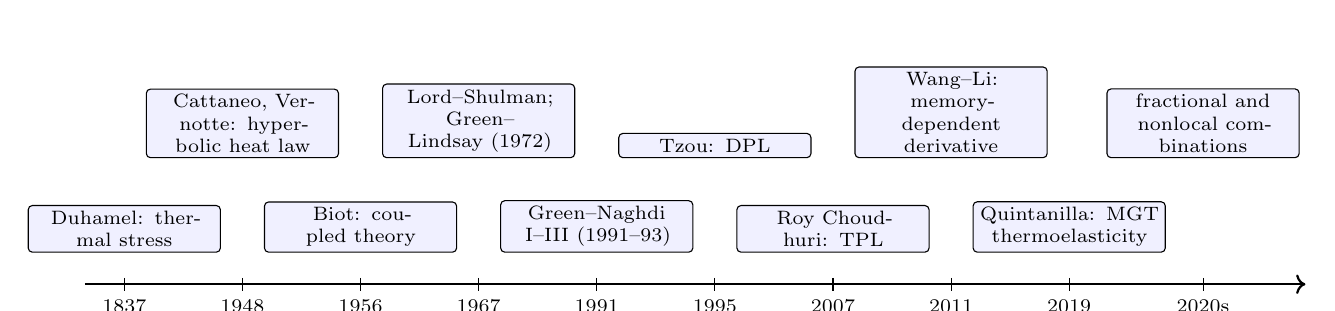
\begin{tikzpicture}[x=1cm,y=1cm,every node/.style={font=\scriptsize},
 ev/.style={draw,rounded corners=1.5pt,fill=blue!6,align=center,inner sep=2pt,text width=2.3cm}]
\draw[->,thick] (0,0)--(15.5,0);
\foreach \x/\l in {0.5/1837,2.0/1948,3.5/1956,5.0/1967,6.5/1991,8.0/1995,9.5/2007,11.0/2011,12.5/2019,14.2/2020s}{\draw (\x,0.08)--(\x,-0.08); \node[below] at (\x,-0.08) {\l};}
\node[ev,above] at (0.5,0.4) {Duhamel: thermal stress};
\node[ev,above] at (2.0,1.6) {Cattaneo, Vernotte: hyperbolic heat law};
\node[ev,above] at (3.5,0.4) {Biot: coupled theory};
\node[ev,above] at (5.0,1.6) {Lord--Shulman; Green--Lindsay (1972)};
\node[ev,above] at (6.5,0.4) {Green--Naghdi I--III (1991--93)};
\node[ev,above] at (8.0,1.6) {Tzou: DPL};
\node[ev,above] at (9.5,0.4) {Roy Choudhuri: TPL};
\node[ev,above] at (11.0,1.6) {Wang--Li: memory-dependent derivative};
\node[ev,above] at (12.5,0.4) {Quintanilla: MGT thermoelasticity};
\node[ev,above] at (14.2,1.6) {fractional and nonlocal combinations};
\end{tikzpicture}}
\caption{Milestones in the theory of thermoelastic waves. Dates are those of the cited original publications (Cattaneo 1948, Vernotte 1958, Biot 1956, Lord--Shulman 1967, Green--Lindsay 1972, Green--Naghdi 1991--1993, Tzou 1995, Roy Choudhuri 2007, Wang--Li 2011, Quintanilla 2019).}\label{fig:timeline}
\end{figure}

\subsection{A map of the contemporary literature}
The recent literature on wave problems in thermoelastic and multiphysics media can be sorted along three largely independent axes: the \emph{heat-flux law}, the \emph{constitutive enrichment} (nonlocal, gradient, microstructural, multiphysics), and the \emph{problem type} (plane waves, surface waves, reflection and transmission, transient response). A typical paper chooses one entry on each axis and computes dispersion curves or response histories. \Cref{tab:streams} lists representative works from our reference list by problem type; the sorting is editorial and many papers appear in more than one row.

\begin{table}[t]\centering\small
\caption{Representative literature by problem type and constitutive enrichment (selection from the reference list; classification by the titles and stated subjects of the works).}\label{tab:streams}
\begin{tabularx}{\textwidth}{@{}p{3.2cm}X@{}}\toprule
Problem type & Representative works\\\midrule
Plane waves, stability, dispersion & Prasad--Kumar \citep{Prasad2020}; Tiwari--Kumar (nonlocal TPL) \citep{Tiwari2021}; van der Merwe--van Rensburg (modal comparison of heat laws) \citep{vanDerMerwe2021}; Sarkar et al.\ (nonlocal type II) \citep{Sarkar2019}.\\
Surface waves & Biswas (porous nonlocal, orthotropic; piezothermoelastic layer) \citep{Biswas2020a,Biswas2020}; Tung (nonlocal piezoelastic Rayleigh) \citep{Tung2019}; Gupta et al.\ (nonlocal piezo-semiconductor Rayleigh wave) \citep{Gupta2024}; Aldandani et al.\ \citep{Aldandani2026}; Ivanov--Savova (energy flux of surface waves) \citep{IvanovSavova1991}.\\
Reflection at free or insulated boundaries & Das et al.\ \citep{Das2008}; Kalkal et al.\ (nonlocal micropolar with rotation) \citep{Kalkal2020}; Singh--Guha (piezothermoelastic fibre-reinforced) \citep{Singh2020b}; Yadav et al.\ \citep{Yadav2023}; Gupta et al.\ \citep{Gupta2024a}; Singh et al.\ (flexoelectric) \citep{Singh2020c}; Jiao et al.\ (flexomagnetic) \citep{Jiao2024}.\\
Interfaces and energy partition & Barak et al.\ \citep{Barak2023,Barak2023IJP,Barak2023JTS,Barak2023MMMS}; Gupta--Kumar \citep{Gupta2023IJNMF,Gupta2023Energy}; Kumar et al.\ \citep{Kumar2023PhysScr,Kumar2019,Kumar2022,Kumar2024,Kumar2024a,Kumar2025,KumarKansal2017,Kumar2018}; Fu--Wei (micropolar imperfect interface) \citep{Fu2013}; Liu et al.\ (graded piezoelectric) \citep{Liu2020}.\\
Transient response, rods, bodies & Singh--Pal \citep{Singh2019,Singh2020a}; Biswas \citep{Biswas2019}; Sur et al.\ \citep{Sur2019,Sur2025}; Bayones et al.\ \citep{Bayones2021}; Li et al.\ (laser pulse, bilayer) \citep{Li2019}; Abouelregal \citep{Abouelregal2023,Abouelregal2020,Abouelregal2020a}; Lata et al.\ \citep{Lata2020}.\\
Damping in resonators & Yang et al.\ (DPL damping in nonlocal nanoplates) \citep{Yang2021}; Kumar--Devi (couple stress plates) \citep{Kumar2017}.\\
Fractional and memory models & Povstenko \citep{Povstenko2004,Povstenko2009,Povstenko2011Cattaneo,Povstenko2016}; Sherief et al.\ \citep{Sherief2010Fractional}; Ezzat--El-Karamany \citep{Ezzat2011}; Wang--Li \citep{Wang2011,Wang2021,WangLi2025IV}; Yu et al.\ \citep{Yu2024}; Bachher--Sarkar \citep{Bachher2019}.\\
Size effects & Eringen \citep{Eringen1972,Eringen1983}; Aifantis \citep{Aifantis1992}; Askes--Aifantis \citep{Askes2006,Askes2011}; Maranganti--Sharma \citep{Maranganti2006,Maranganti2007}; Lazar--Agiasofitou \citep{Lazar2022}; Zang et al.\ \citep{Zang2014}; Li et al.\ \citep{Li2018}.\\
Variational and uniqueness theory & Marotti de Sciarra \citep{Marotti2013}; Srivastava--Mukhopadhyay \citep{Srivastava2026}; Chandrasekharaiah \citep{Chandrasekharaiah1996}; Chiri\c{t}\u{a} et al.\ \citep{Chirita2016,Tibullo2017}.\\
\bottomrule\end{tabularx}
\end{table}

\subsection{Recurrent observations from the literature}
Reading across these streams, we note patterns that shape the rest of this review.
\begin{itemize}
\item \textbf{The heat law and the elastic enrichment are treated as independent modules.} Most interface and surface-wave papers combine one of several heat laws with one of several enrichments, so the dispersion relations differ only through $G(s)$ and through the elastic operator. This is why a unified treatment is possible and why a limit-checking discipline matters.
\item \textbf{Energy ratios and amplitude ratios dominate the reflection literature.} The interface papers cited above report energy ratios, whose sum must equal one in a lossless setting. A sum different from one is therefore a diagnostic of either dissipation, an error in the flux definition, or both; Section~\ref{sec:interfaces} discusses this check in detail.
\item \textbf{Parameter values are rarely tied to measurements.} Lags and fractional orders are typically assigned convenient values, so many figures demonstrate a model rather than a material.
\item \textbf{The thermodynamic status of the Taylor-expanded models is delicate.}

\begin{summarybox}[Summary]
The historical line runs Fourier (parabolic) $\to$ Cattaneo/vernotte (flux relaxation) $\to$ Lord--Shulman $\to$ Green--Lindsay $\to$ Green--Naghdi types I--III $\to$ dual-phase-lag $\to$ three-phase-lag $\to$ Moore--Gibson--Thompson $\to$ fractional and memory-dependent laws. Each step adds one modelling ingredient (relaxation time, second temperature, thermal displacement, lag on temperature gradient, inertia term, memory kernel). Recurrent pitfalls: unmeasured lag parameters, Taylor truncation passed off as exact, mode-flux sums mistaken for energy conservation, GN-III confused with a finite-speed theory.
\end{summarybox} The papers of Chiri\c{t}\u{a} and co-workers \citep{Chirita2016,Tibullo2017} examine thermodynamic compatibility and continuous dependence of the time-differential lag models, and our own stability computation (Section~\ref{sec:lags}) shows how strongly the truncation order matters.
\end{itemize}

\section{Thermomechanical foundations}\label{sec:foundations}
This section collects the balance laws, the thermodynamic structure of linear thermoelasticity, the reasons why Fourier's law is problematic for fast processes, and the heat-flux template that organises the remainder of the review. It is self-contained so that the later sections can refer to equation numbers rather than rederive.

\subsection{Balance laws for small disturbances}
Let a body occupy a region $\Omega$ and let $\bu(\bx,t)$ be the displacement from a reference state at uniform temperature $T_0$ and zero stress. For small displacement gradients the strain is $\varepsilon_{ij}=\tfrac12(u_{i,j}+u_{j,i})$. The local forms of the balance of linear momentum and of energy are
\begin{align}
\rho\,\ddot u_i &= \sigma_{ij,j}+\rho f_i, \label{eq:mom}\\
\rho\,\dot e &= \sigma_{ij}\dot\varepsilon_{ij}-q_{i,i}+\rho r, \label{eq:first}
\end{align}
where $\rho$ is the (reference) density, $f_i$ the body force per unit mass, $e$ the specific internal energy, $q_i$ the heat flux and $r$ the heat supply per unit mass. Balance of angular momentum implies a symmetric stress in the absence of couple stresses. The second law, in the Clausius--Duhem form used by Coleman and Noll \citep{Coleman1963},
\begin{equation}
\rho\,\dot\eta \;\ge\; \frac{\rho r}{T}-\Bigl(\frac{q_i}{T}\Bigr)_{,i}, \label{eq:CD}
\end{equation}
with specific entropy $\eta$ and absolute temperature $T$, restricts the constitutive relations. Eliminating $r$ between \eqref{eq:first} and \eqref{eq:CD} and introducing the Helmholtz free energy $\psi=e-T\eta$ gives
\begin{equation}
-\rho\bigl(\dot\psi+\eta\dot T\bigr)+\sigma_{ij}\dot\varepsilon_{ij}-\frac{q_i T_{,i}}{T}\;\ge\;0. \label{eq:CDpsi}
\end{equation}
For a material with $\psi=\psi(\varepsilon_{ij},T)$, \eqref{eq:CDpsi} must hold for arbitrary $\dot\varepsilon_{ij}$ and $\dot T$; the coefficients of those rates must vanish,
\begin{equation}
\sigma_{ij}=\rho\,\frac{\partial\psi}{\partial\varepsilon_{ij}},\qquad \eta=-\frac{\partial\psi}{\partial T},\label{eq:coleman}
\end{equation}
and the remaining term gives the \emph{heat-conduction inequality}
\begin{equation}
q_iT_{,i}\;\le\;0.\label{eq:cond-ineq}
\end{equation}
Fourier's law $q_i=-k_{ij}T_{,j}$ with positive-semidefinite $k_{ij}$ satisfies \eqref{eq:cond-ineq} identically; so does any law for which the flux is, to leading order, opposed to the temperature gradient. This is the point at which lagged and relaxed laws require care (Section~\ref{sec:beyond}).

\subsection{Linear thermoelasticity}
Expanding $\rho\psi$ to second order about $(\varepsilon_{ij},T)=(0,T_0)$, with $\theta=T-T_0$, gives
\begin{equation}
\rho\psi=\tfrac12C_{ijkl}\varepsilon_{ij}\varepsilon_{kl}-\beta_{ij}\varepsilon_{ij}\theta-\frac{\rho c}{2T_0}\theta^2,\label{eq:psi}
\end{equation}
where $C_{ijkl}$ are the isothermal elastic moduli, $\beta_{ij}$ the thermal-stress tensor and $c$ the specific heat at constant strain (we do not carry the constant and linear terms in $\theta$, which only fix the reference values of the energy and entropy). Equations~\eqref{eq:coleman} give
\begin{equation}
\sigma_{ij}=C_{ijkl}\varepsilon_{kl}-\beta_{ij}\theta,\qquad \rho\eta=\beta_{ij}\varepsilon_{ij}+\frac{\rho c}{T_0}\theta.\label{eq:stress}
\end{equation}
The first of these is the Duhamel--Neumann relation. For an isotropic solid $C_{ijkl}=\lambda\delta_{ij}\delta_{kl}+\mu(\delta_{ik}\delta_{jl}+\delta_{il}\delta_{jk})$ and $\beta_{ij}=\beta\delta_{ij}$ with $\beta=(3\lambda+2\mu)\alpha_T$, since free thermal expansion $\varepsilon_{ij}=\alpha_T\theta\,\delta_{ij}$ must produce zero stress: $\sigma_{ij}=(3\lambda+2\mu)\alpha_T\theta\,\delta_{ij}-\beta\theta\,\delta_{ij}=0$. The energy balance $\rho T\dot\eta=-q_{i,i}+\rho r$ (entropy form of \eqref{eq:first} when the stress power is accounted for by the free energy), linearised about $T_0$ using the second of \eqref{eq:stress}, gives
\begin{equation}
\rho c\,\dot\theta+T_0\,\beta_{ij}\dot\varepsilon_{ij}=-q_{i,i}+\rho r. \label{eq:en}
\end{equation}
Together with \eqref{eq:mom}, \eqref{eq:stress} and a heat-flux law, \eqref{eq:en} closes the system. The coefficients carry a clear physical reading: $\rho c$ is the heat capacity per unit volume at constant strain; $T_0\beta^2/(\rho c)$ is the difference between the adiabatic and isothermal longitudinal moduli, namely
\begin{equation}
\lambda_{\rm ad}+2\mu_{\rm ad}=\lambda+2\mu+\frac{T_0\beta^2}{\rho c},
\qquad\text{equivalently}\qquad c_{\rm ad}^2=c_1^2\,(1+\varepsilon),\quad \varepsilon=\frac{\beta^2T_0}{\rho^2c\,c_1^2}. \label{eq:adiabatic}
\end{equation}
Table~\ref{tab:materials} gives the coupling parameter $\varepsilon$ and the characteristic frequency $\omega_*=\rho c c_1^2/k$ for representative solids. The coupling is of order $10^{-2}$ for common metals and much smaller for low-expansion materials; the characteristic frequency lies far above the ultrasonic range for bulk solids ($10^{10}$--$10^{12}$ Hz) and drops into the megahertz--gigahertz range only when waves are confined to micro-scale structures (Section~\ref{sec:applications}).
\begin{table}[ht]\centering\small
\caption{Thermoelastic coupling $\varepsilon$ and characteristic frequency $f_*=\omega_*/2\pi$ computed from rounded handbook-type values (300\,K) of density, specific heat, conductivity, expansion coefficient, Young's modulus and Poisson ratio; the reader should replace them by data for the specimen at hand.}\label{tab:materials}
\begin{tabular}{@{}lrrrr@{}}\toprule
Material & $c_1$ (m/s) & $\varepsilon$ & $f_*=\omega_*/2\pi$ (Hz) & $\alpha=k/\rho c$ (m$^2$/s)\\\midrule
Aluminium & 6198 & 0.027 & $6.3\times10^{10}$ & $9.8\times10^{-5}$\\
Copper & 4540 & 0.019 & $2.8\times10^{10}$ & $1.2\times10^{-4}$\\
Silicon & 8854 & 0.00056 & $1.4\times10^{11}$ & $9.2\times10^{-5}$\\
Steel (carbon) & 5778 & 0.0097 & $4.1\times10^{11}$ & $1.3\times10^{-5}$\\
Fused silica & 5972 & 7.2e-06 & $6.6\times10^{12}$ & $8.6\times10^{-7}$\\
\bottomrule\end{tabular}
\end{table}

\subsection{Beyond Fourier's law}\label{sec:beyond}
\paragraph{Why Fourier's law is parabolic.} Inserting $q_i=-kT_{,i}$ in \eqref{eq:en} with constant coefficients and no coupling gives $\rho c\,\dot\theta=k\nabla^2\theta$. The fundamental solution is a Gaussian that is nonzero at all distances for every positive time, so the signal speed is unbounded. Because the Gaussian decays so rapidly, the infinite speed has no observable consequence for slow processes; for processes on the time scale of the carrier relaxation it has.

\paragraph{Relaxation of the flux.} A natural modification, due to Cattaneo and Vernotte \citep{Cattaneo1948,Vernotte1958}, lets the flux relax to its Fourier value with relaxation time $\tau_0$:
\begin{equation}
q_i+\tau_0\dot q_i=-k\,\theta_{,i}.\label{eq:cattaneo}
\end{equation}
With \eqref{eq:en} and no coupling, $k\nabla^2\theta=\rho c(\dot\theta+\tau_0\ddot\theta)$, a damped wave equation with front speed $c_T=\sqrt{k/(\rho c\tau_0)}$. In kinetic terms $\tau_0$ is the mean time between momentum-destroying collisions of the heat carriers and $c_T$ is of the order of the carrier speed divided by $\sqrt3$ in three dimensions; in phonon hydrodynamics a different, ``second sound'', regime exists in which normal (momentum-conserving) collisions dominate \citep{GuyerKrumhansl1966,GuyerKrumhansl1966II,Chester1963}.

\paragraph{Thermodynamic compatibility via extended irreversible thermodynamics.} The Cattaneo law does not follow from \eqref{eq:CD} with a free energy that depends only on $(\varepsilon_{ij},T)$: the flux must enter the state space. In extended irreversible thermodynamics \citep{Jou2010,MuellerRuggeri1998,Mueller1967} the entropy depends also on $q_i$. In one dimension, without deformation, take
\begin{equation}
\eta=\eta_{\rm eq}(e)-\frac{\tau_0}{2\rho kT^2}\,q^2,\qquad \rho\dot e=-q_{,x}
\end{equation}
and an entropy flux $q/T$. Then
\begin{equation}
\rho\dot\eta+\Bigl(\frac qT\Bigr)_{,x}=-\frac{q}{kT^2}\bigl(\tau_0\dot q+kT_{,x}\bigr),
\end{equation}
and for the Cattaneo law the bracket equals $-q$, so the entropy production is $q^2/(kT^2)\ge0$. This is the minimal sense in which the relaxed law is thermodynamically admissible: the entropy contains a quadratic correction in the flux. The correction is of second order in the disturbance, which is why the linear theory is not sensitive to it. In lagged models the corresponding entropy functional has to be constructed model by model, and for some Taylor truncations of the lag equations no admissible functional exists unless parameter restrictions hold \citep{Chirita2016,Tibullo2017}.

\paragraph{Thermal displacement and the Green--Naghdi route.} Green and Naghdi \citep{Green1991,Green1993} take instead an entropy \emph{balance} with an entropy flux and postulate constitutive relations in terms of the \emph{thermal displacement} $v$, $\dot v=\theta$ (so $v=\int\theta\,\dd t$). The flux $q_i$ may depend on $\theta_{,i}$ and $v_{,i}$; type II ($q_i=-k^*v_{,i}$) conserves energy, type III adds Fourier dissipation. In wave problems $v$ is the natural field since $\hat v=\hat\theta/s$.

\paragraph{Green--Lindsay: rates in the stress and entropy.} Green and Lindsay \citep{Green1972} keep a single temperature but let the free energy and stress depend on $\dot\theta$ as well, introducing two relaxation times $\tau_0\ge\tau_1\ge0$ in the stress and entropy relations; the heat law remains Fourier's. Solutions of the original theory can exhibit discontinuities at wave fronts that some authors regard as unphysical, and a modification with a strain-rate term has been proposed to remove them \citep{Yu2018ModifiedGL}. Section~\ref{sec:hyperbolic} returns to this theory.

\subsection{The heat-flux template}\label{sec:framework-link}
Linear wave problems with constant coefficients depend on the heat-flux law only through its Laplace-domain relation between flux and temperature gradient. We therefore define the family
\begin{equation}
q_i+\tau_q\,\dot q_i=-k\,\bigl(\theta_{,i}+\tau_T\,\dot\theta_{,i}\bigr)-k^{*}\bigl(v_{,i}+\tau_v\,\dot v_{,i}\bigr),\qquad \dot v=\theta,\label{eq:template}
\end{equation}
and note that after Laplace transformation (zero initial data)
\begin{equation}
\hat q_i=-G(s)\,\hat\theta_{,i},\qquad
G(s)=\frac{k\,(1+\tau_Ts)+k^{*}(1+\tau_vs)/s}{1+\tau_qs}.\label{eq:G}
\end{equation}

\begin{figure}[t!]\centering\small
% fig1_template.tex -- Heat-flux template geometry (s03_foundations)
% Style: consistent across all figures -- same colours, fonts, arrows
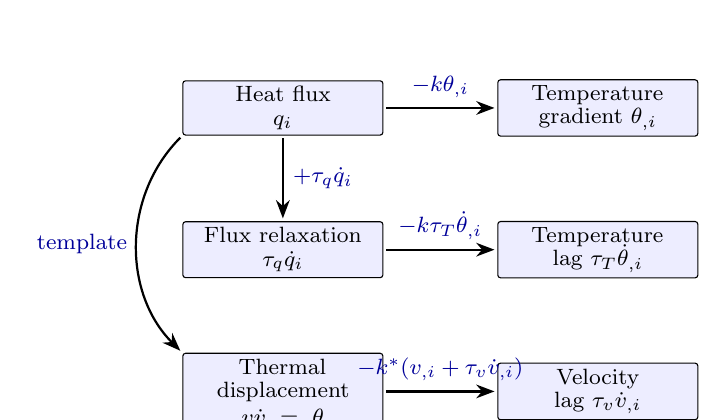
\begin{tikzpicture}[x=1.0cm,y=1.0cm,>=Stealth]
  % Consistent node style
  \tikzset{
    node/.style={draw,rounded corners=1pt,fill=blue!7,align=center,font=\footnotesize,inner sep=2pt,text width=2.4cm},
    arr/.style={->,thick,shorten >=1pt,shorten <=1pt},
    lbl/.style={font=\footnotesize,text=blue!60!black},
  }
  % Explicitly positioned nodes (no right=of)
  \node[node] at (-3.2, 0.0) (flux) {Heat flux\\[-1pt] $q_i$};
  \node[node] at ( 0.8, 0.0) (grad) {Temperature\\[-1pt] gradient $\theta_{,i}$};
  \node[node] at (-3.2,-1.8) (lag) {Flux relaxation\\[-1pt] $\tau_q\dot q_i$};
  \node[node] at ( 0.8,-1.8) (tlag) {Temperature\\[-1pt] lag $\tau_T\dot\theta_{,i}$};
  \node[node] at (-3.2,-3.6) (v) {Thermal\\[-1pt] displacement $v$\n$\dot v=\theta$};
  \node[node] at ( 0.8,-3.6) (vlag) {Velocity\\[-1pt] lag $\tau_v\dot v_{,i}$};
  % Arrows with labels at pos=0.5
  \draw[arr] (flux.east) -- (grad.west) node[pos=0.5,above,lbl] {$-k\theta_{,i}$};
  \draw[arr] (lag.east) -- (tlag.west) node[pos=0.5,above,lbl] {$-k\tau_T\dot\theta_{,i}$};
  \draw[arr] (v.east) -- (vlag.west) node[pos=0.5,above,lbl] {$-k^*(v_{,i}+\tau_v\dot v_{,i})$};
  \draw[arr] (flux.south) -- (lag.north) node[pos=0.5,right,lbl] {$+\tau_q\dot q_i$};
  \draw[arr] (flux.south west) to[out=-135,in=135] node[pos=0.5,left,lbl] {template} (v.north west);
\end{tikzpicture}

\caption{Geometry after \citep{Biot1956}: the heat-flux template couples the flux to temperature gradients through relaxation and lags. Each theory sets some terms to zero.}\label{fig:template}
\end{figure}

\Cref{tab:param} lists the parameter choices that reproduce the principal models. For fractional and memory-dependent models $G(s)$ has the same structure with $s$ replaced by non-integer powers or by kernel transforms (Section~\ref{sec:memory}).

\begin{table}[ht]\centering\small
\caption{Heat-flux theories as parameter choices in the template \eqref{eq:template}. All entries use the energy balance \eqref{eq:en}.}\label{tab:param}
\begin{tabular}{@{}lccccc l@{}}\toprule
Theory & $k$ & $k^*$ & $\tau_q$ & $\tau_T$ & $\tau_v$ & Source\\\midrule
Classical (Fourier) & $k$ & 0 & 0 & 0 & 0 & \citep{Biot1956}\\
Lord--Shulman (Cattaneo) & $k$ & 0 & $\tau_0$ & 0 & 0 & \citep{Lord1967,Cattaneo1948,Vernotte1958}\\
Dual-phase-lag (DPL), 1st order & $k$ & 0 & $\tau_q$ & $\tau_T$ & 0 & \citep{Tzou1995,Tzou1997}\\
Green--Naghdi II & 0 & $k^*$ & 0 & 0 & 0 & \citep{Green1993}\\
Green--Naghdi III & $k$ & $k^*$ & 0 & 0 & 0 & \citep{Green1991}\\
Three-phase-lag (TPL) & $k$ & $k^*$ & $\tau_q$ & $\tau_T$ & $\tau_v$ & \citep{RoyChoudhuri2007}\\
MGT (flux form) & $k$ & $k^*$ & $\tau_q$ & 0 & 0 & \citep{Quintanilla2019}\\\bottomrule
\end{tabular}
\end{table}

\paragraph{Exact reductions and singular limits.} The function $G(s)$ determines which reductions are regular. The following were verified symbolically (script \path{check_reductions.py}).
\begin{itemize}
\item \textbf{DPL $\to$ Lord--Shulman:} $\tau_T\to0$ with $\tau_q=\tau_0$ fixed, $k^*=0$. Letting $\tau_q\to0$ with $\tau_T$ fixed gives instead $G=k(1+\tau_Ts)$, a Fourier law with a temperature-rate term (Kelvin--Voigt-like conduction), not Cattaneo.
\item \textbf{TPL $\to$ DPL:} $k^*\to0$. For $k^*\ne0$ the function $G(s)\sim k^*/s$ as $s\to0$, so the low-frequency and long-time response is qualitatively different.
\item \textbf{TPL $\to$ classical:} $k^*\to0$ and all three lags $\to0$.
\item \textbf{GN-II:} $k=0$, all lags zero, $G=k^*/s$; \textbf{GN-III:} all lags zero, $G=k+k^*/s$.
\item \textbf{Large-$s$ behaviour.} $G(\infty)=0$ for Lord--Shulman (hyperbolic behaviour, finite thermal speed $c_T$); $G(\infty)=k\tau_T/\tau_q$ for DPL (diffusive again at high frequency with effective conductivity $k\tau_T/\tau_q$).
\item \textbf{Fractional orders:} the endpoint $\alpha\to2$ of the Caputo family is second order in time and is not Fourier's law (Section~\ref{sec:memory}).
\end{itemize}

\subsection{Energy balance and energy flux}\label{sec:energy}
For the Lord--Shulman model in the absence of body forces and heat supply, multiplying \eqref{eq:mom} by $\dot u_i$, \eqref{eq:en} by $\theta/T_0$ and using \eqref{eq:cattaneo} gives
\begin{equation}
\frac{\partial\mathcal E}{\partial t}+P_{i,i}=-\frac{q_iq_i}{kT_0},\qquad
\mathcal E=\tfrac12\rho\dot u_i\dot u_i+\tfrac12C_{ijkl}\varepsilon_{ij}\varepsilon_{kl}+\frac{\rho c}{2T_0}\theta^2+\frac{\tau_0}{2kT_0}q_iq_i,\label{eq:energy}
\end{equation}
\begin{equation}
P_i=-\sigma_{ij}\dot u_j+\frac{\theta\,q_i}{T_0}.\label{eq:P}
\end{equation}
Here $\mathcal E$ is positive definite and $P_i$ is the flux associated with it; the right-hand side is the dissipation. This quadratic (availability-type) energy and its flux $P_i$ are what is meant by ``energy flux'' in linear wave theory; they differ from the flux $q_i-\sigma_{ij}\dot u_j$ of the \emph{total} internal energy, whose heat-flux part is first order in the disturbance and averages to zero over a period. For the classical theory the same procedure gives \eqref{eq:energy} without the last term in $\mathcal E$. For the other members of the template an energy functional exists under parameter conditions that must be stated for each model: for Green--Naghdi type II the functional is conserved; for DPL and TPL (first-order truncations) the construction is more involved \citep{Quintanilla2003DPL,Chirita2016}. We use \eqref{eq:P} for interface energy partition in Section~\ref{sec:interfaces}.


\begin{summarybox}[Summary]
The balance laws \eqref{eq:mom}\textendash\eqref{eq:en}, the Coleman--Noll relations \eqref{eq:coleman} and the conduction inequality \eqref{eq:cond-ineq} close the system once a heat-flux law is supplied. Fourier's law is parabolic; relaxed and lagged laws give finite-speed thermal waves. The template \eqref{eq:template} reduces to classical, LS, DPL, TPL, GN-II/III and MGT by setting its parameters, but the endpoint $\tau_q\to0$ with $\tau_T$ fixed is singular (Kelvin--Voigt-like conduction, not Cattaneo). Energy is conserved exactly only for GN-II.
\end{summarybox}
\section{Kinetic origin of the hyperbolic and Guyer--Krumhansl laws}\label{sec:kinetic}

The lag models of \cref{sec:lags} are usually justified by their formal structure. Their physical meaning comes from kinetic theory of phonons, and this section summarises how the two most-used laws arise there. We state standard results of phonon hydrodynamics at the level of structure; coefficient values depend on the dispersion model and should be taken from the original derivations.

\subsection{Relaxation-time closure and the Cattaneo law}
Write the linearised phonon Boltzmann equation for the deviation $n'$ from equilibrium with a single relaxation time $\tau_R$ for momentum-destroying (resistive) scattering. Taking the first moment, with the energy flux $q$ as the moment variable, and using the first-order closure that the second moment is proportional to the temperature gradient, gives
\begin{equation}\label{eq:cattkin}
\tau_R\,\dot q+q=-k\,\nabla\theta,\qquad k=\tfrac13 c_v v^2\tau_R ,
\end{equation}
where $v$ is the phonon group speed. This is the Cattaneo law with $\tau_q=\tau_R$. It is valid when the closure holds, namely when the phonon mean free path is small compared with the wavelength, so that $\omega\tau_R\ll1$ and $\ell_{\rm mfp}k\ll1$. Beyond this the closure fails, and the finite speed $\sqrt{k/(c_v\tau_R)}=v/\sqrt3$ should not be expected to describe a ballistic front.

\subsection{Normal scattering and the Guyer--Krumhansl law}
If momentum-conserving (normal) collisions with time $\tau_N$ dominate over resistive ones, $\tau_N\ll\tau_R$, the expansion to the next order yields the Guyer--Krumhansl equation
\begin{equation}\label{eq:GKkin}
\tau_R\,\dot q+q=-k\,\nabla\theta+\ell^{2}\bigl(\nabla^{2}q+2\nabla\nabla\!\cdot q\bigr),
\end{equation}
with a length $\ell$ of order $v\sqrt{\tau_N\tau_R}$ up to a model-dependent numerical factor ($1/5$ in a common Debye-type derivation). In one dimension the bracket becomes $3q_{,xx}$. Together with $c_v\dot\theta=-q_{,x}$ the uncoupled dispersion relation is
\begin{equation}\label{eq:GKdisp}
k_w^{2}=-\,\frac{c_v\,s\,(1+\tau_R s)}{k+3\ell^{2}c_v s},\qquad s=-i\omega .
\end{equation}
The law \cref{eq:GKkin} is not of the form $\hat q=-G(s)\hat\theta_{,x}$ with $G$ independent of $k_w$: the Laplacian term makes the response wavenumber dependent. It is therefore outside the template of \cref{sec:foundations} and is treated separately in \cref{sec:size}. The practical consequence is that size effects and relaxation effects cannot be separated by choosing different $G(s)$.


\subsection{Dispersion of the Guyer--Krumhansl law}
\Cref{fig:gk} (script \path{scripts/fig_gk.py}) compares the uncoupled thermal branch for the Fourier, Cattaneo and Guyer--Krumhansl laws, in units with $\chi=k/c_v=1$ and $\tau_R=1$. Reading the numbers at $\omega\tau_R=0.1,\,1,\,10,\,100$:
\begin{itemize}
\item Fourier: phase speed $0.45,\,1.41,\,4.48,\,14.1$ (in units of $\sqrt{\chi/\tau_R}$), growing as $\sqrt{\omega}$, and attenuation $\operatorname{Im}k_w=0.22,\,0.71,\,2.2,\,7.1$.
\item Cattaneo ($\ell=0$): $0.43,\,0.91,\,1.00,\,1.00$, i.e.\ the speed saturates at $\sqrt{\chi/\tau_R}$, and the attenuation saturates at $1/(2\sqrt{\chi\tau_R})=0.5$.
\item Guyer--Krumhansl with $\ell^2=0.05$: $0.43,\,0.95,\,1.57,\,5.3$ and attenuation $0.22,\,0.53,\,3.9,\,18$; with $\ell^2=0.3$: $0.45,\,1.34,\,4.2,\,13.4$ and attenuation $0.22,\,0.71,\,2.3,\,7.4$.
\end{itemize}
At low frequency the three laws coincide with diffusion. At high frequency the Cattaneo law approaches a finite front, whereas the Guyer--Krumhansl law returns to diffusive behaviour: from \cref{eq:GKdisp}, $k_w^2\to i\omega\tau_R/(3\ell^2)$ for $\omega\to\infty$, so both $\operatorname{Re}k_w$ and $\operatorname{Im}k_w$ grow as $\sqrt{\omega}$ and the phase speed grows as $\sqrt{6\ell^2\omega/\tau_R}$ (confirmed numerically to $0.2\%$). The linear Guyer--Krumhansl law therefore has no finite signal speed in this uncoupled form. Its role is to represent non-local (Knudsen-type) corrections at intermediate frequencies, not to enforce a front.

\begin{figure}[t]
\centering
\includegraphics[width=\linewidth]{figs/fig_gk.pdf}
\caption{Thermal branch for Fourier, Cattaneo and Guyer--Krumhansl laws ($\chi=\tau_R=1$): (a) phase speed, (b) attenuation. The dispersion relation is \cref{eq:GKdisp}.}
\label{fig:gk}
\end{figure}
\subsection{What this means for model choice}
(i) A lag law is a statement about relaxation of the flux; if the heat-carrier mean free path is comparable to the sample, the Guyer--Krumhansl structure or a full kinetic model is the physical starting point. (ii) Parameters $\tau_q$, $\tau_T$ obtained by fitting a lag law to transient data are effective and need not equal a microscopic relaxation time. (iii) A lag law with $\tau_q$ of the order of $10^{-12}$\,s describes phonon relaxation only if a closure of the type above is valid at the wavelengths and frequencies of interest.

\section{Mathematical preliminaries}\label{sec:prelim}

The later sections use a small set of tools repeatedly. They are collected here with the conventions of this review, so that every statement about branches, damping and dispersion has a single definition.

\subsection{Fourier--Laplace conventions}
Fields depend on $\exp[i(kx-\omega t)]$ and the Laplace variable is $s=-i\omega$, so that $\partial_t\to s$ and $\partial_x\to ik$. For a causal response, i.e.\ one that vanishes before the excitation, the transfer functions $G(s)$ and the resulting $k(\omega)$ are analytic in the upper half of the complex $\omega$-plane ($\operatorname{Re}s>0$). Two consequences are used below: the wave number is determined by $k^2=-\rho c\,s/G(s)$ for the uncoupled thermal branch, and the appropriate root is the one whose spatial amplitude does not grow, $\operatorname{Im}k\ge0$, with $\operatorname{Re}k>0$ for propagation in $+x$.

\subsection{Branches and the choice of root}
The dispersion relation is a polynomial in $K=k^2$ with coefficients depending on $s$, so each root $K_j(s)$ gives two wave numbers $\pm\sqrt{K_j}$. The rules adopted are: (i) for each $K_j$, take the square root with $\operatorname{Im}k\ge0$; (ii) a ``branch'' is a $k(\omega)$ followed continuously in $\omega$, because the labels ``elastic-type'' and ``thermal-type'' are meaningful only away from hybridisation, where roots approach each other; (iii) near hybridisation, which in the Lord--Shulman model occurs for $\tau\omega_*\approx1$, tracking by continuity with a sufficiently fine frequency grid is necessary, and selecting the root nearest an expected value fails. Both failures were met in producing the figures of this review.

\subsection{Spatial and temporal damping}
Two measures of loss appear. For real $\omega$ and complex $k$ one defines $Q_x^{-1}=2\operatorname{Im}k/\operatorname{Re}k$; for real $k$ and complex $\omega$ one defines $Q_t^{-1}=2|\operatorname{Im}\omega|/|\operatorname{Re}\omega|$. For weak damping the two are related by the group-to-phase velocity ratio, $Q_t^{-1}\simeq(v_g/v_p)\,Q_x^{-1}$. In the clamped-bar example of \cref{sec:bar} the classical peak $Q_t^{-1}=0.0488$ at $\varepsilon=0.1$ compares with the Debye value $\varepsilon/2=0.05$ of the spatial measure; the difference is a few percent and is of the order $\varepsilon$ expected from that relation. Resonator experiments measure $Q_t$, wave-propagation experiments $Q_x$, and the two should not be compared without the conversion.

\subsection{Causality and the sum rule}
A causal response obeys the Kramers--Kronig relations, which tie dispersion to loss: a medium with a loss peak must show a change of speed. For weak damping the relation takes the form of a sum rule,
\begin{equation}\label{eq:sumrule}
\int_0^\infty Q_x^{-1}\,d\ln\omega=\pi\,\frac{v_0-v_\infty}{\bar v},
\end{equation}
where $v_0$ and $v_\infty$ are the phase speeds at zero and infinite frequency and $\bar v$ is their mean. For the Debye form $Q^{-1}=\varepsilon x/(1+x^2)$ the left side is $\pi\varepsilon/2$ and the right side is $\pi(\sqrt{1+\varepsilon}-1)\approx\pi\varepsilon/2$, which is consistent with the adiabatic and isothermal speeds of \cref{sec:classical}. We checked \cref{eq:sumrule} numerically on the exact coupled classical dispersion relation (script \path{scripts/check_kk.py}): at $\varepsilon=0.01$ the integral is $1.562994\times10^{-2}$ against $1.562991\times10^{-2}$ on the right, and at $\varepsilon=0.001$ the two sides are $1.570009\times10^{-3}$ and $1.570011\times10^{-3}$. The practical use is as a consistency test on any computed or measured loss curve: if a model predicts a loss peak but no corresponding speed change, or the reverse, it violates causality or has been truncated inconsistently.

\subsection{Support of the solution and finite signal speed}
The Laplace transform of a solution supported in $x\le ct$ decays as $e^{-sx/c}$ for $\operatorname{Re}s\to\infty$. Conversely, a transfer function with $k(s)\sim s/c$ at large $s$ implies a front travelling at $c$, which is the origin of the criterion used in \cref{sec:hyperbolic}: finite signal speed requires $sG(s)$ to tend to a finite, non-zero limit. Models for which $k_w\sim\sqrt{s}$ at large $s$ (classical, DPL, TPL, GN-III, and the Guyer--Krumhansl law of \cref{sec:kinetic}) have no front, and a transient problem for them has a solution that is nonzero everywhere immediately after the excitation, however small.

\subsection{Complex roots of the delay law}
When $G$ contains an exponential, as in the exact delay law of \cref{sec:delayfid}, $k^2=-\rho c\,s/G(s)$ is an entire function times $s$ and has infinitely many branches. Truncations replace this by a rational function with finitely many roots. Roots of the delay law that the truncation does not contain, and spurious roots that it introduces, are a likely reason why truncated and exact laws differ at $\omega\tau\gtrsim1$, although this has to be checked for each truncation.

\section{Classical coupled thermoelasticity}\label{sec:classical}
\subsection{Field equations}
For an isotropic solid with Fourier conduction $q_i=-k\theta_{,i}$, \eqref{eq:mom}, \eqref{eq:stress} and \eqref{eq:en} give the Navier-type system
\begin{align}
\rho\ddot{\bu}&=\mu\nabla^2\bu+(\lambda+\mu)\nabla(\nabla\!\cdot\!\bu)-\beta\nabla\theta+\rho\bm f,\label{eq:navier}\\
\rho c\,\dot\theta&=k\nabla^2\theta-T_0\beta\,\nabla\!\cdot\!\dot{\bu}+\rho r.\label{eq:heateq}
\end{align}
The thermodynamic content is fully encoded in the two coupling terms: the thermal body force $-\beta\nabla\theta$ in \eqref{eq:navier} and the dilatation heating $-T_0\beta\nabla\!\cdot\!\dot{\bu}$ in \eqref{eq:heateq}. Their product, $T_0\beta^2$, is what appears in the single coupling constant $\varepsilon$ of \eqref{eq:adiabatic}; the reciprocal structure (the same $\beta$ in both) is a consequence of the existence of the free energy \eqref{eq:psi}. A sign or factor error in either term breaks the reciprocity and is a common source of unphysical results; in our dispersion checks (Appendix~\ref{app:disp}) this is exactly what a symbolic comparison with the field equations detects.

\paragraph{Helmholtz decomposition.} Writing $\bu=\nabla\phi+\nabla\times\bm\psi$ with $\nabla\!\cdot\!\bm\psi=0$ decouples the problem in an unbounded isotropic body into
\begin{equation}
\rho\ddot\phi=(\lambda+2\mu)\nabla^2\phi-\beta\theta,\qquad
\rho c\dot\theta=k\nabla^2\theta-T_0\beta\nabla^2\dot\phi,\qquad
\rho\ddot{\bm\psi}=\mu\nabla^2\bm\psi.\label{eq:helm}
\end{equation}
The shear potential $\bm\psi$ obeys an uncoupled wave equation with speed $c_2=\sqrt{\mu/\rho}$: transverse waves are neither attenuated nor dispersed by thermoelastic coupling in an unbounded isotropic medium. Only the dilatational potential couples to temperature. At boundaries and interfaces, shear and dilatational motions are coupled again by boundary conditions, which is why surface waves and reflected shear waves are affected by thermal coupling (Sections~\ref{sec:surface} and~\ref{sec:interfaces}).

\begin{figure}[t!]\centering\small
\begin{tikzpicture}[x=1.1cm,y=1.1cm,>=Stealth,
  node/.style={draw,rounded corners=1pt,fill=blue!7,align=center,font=\footnotesize,inner sep=2pt,text width=2.4cm},
  arr/.style={->,thick,shorten >=1pt,shorten <=1pt},
  lbl/.style={font=\tiny\itshape,text=blue!60!black}]
  \node[node] (mech) {Mechanical\\\[-2pt] $\bu,\varepsilon_{ij}$\\\[-2pt] stress $\sigma_{ij}$};
  \node[node,right=1.8cm of mech] (therm) {Thermal\\\[-2pt] $\theta,T_0$\\\[-2pt] flux $q_i$};
  \node[node,below=1.4cm of mech] (energy) {Energy\\\[-2pt] balance\\\[-2pt] $\rho c\dot\theta+T_0\beta\dot\varepsilon_{kk}=-q_{i,i}$};
  \draw[arr] (mech.east) -- (therm.west) node[midway,above,lbl] {$-T_0\beta\nabla\!\cdot\dot{\bu}$};
  \draw[arr] (therm.west) -- (mech.east) node[midway,below,lbl] {$-\beta\nabla\theta$};
  \draw[arr] (mech.south) -- (energy.north) node[midway,left,lbl] {work $\sigma\dot\varepsilon$};
  \draw[arr] (therm.south west) -- (energy.north east) node[midway,right,lbl] {heat $q_i,T$};
\end{tikzpicture}
\caption{Geometry after \citep{Biot1956}: classical coupled thermoelasticity -- mechanical and thermal fields are linked by the thermal body force and dilatation heating, the two terms sharing $\beta$.}\label{fig:classical-coup}
\end{figure}

\subsection{Uniqueness and energy}
Multiplying \eqref{eq:navier} by $\dot u_i$ and \eqref{eq:heateq} by $\theta/T_0$ and integrating gives the energy identity \eqref{eq:energy} without the flux-relaxation term, with dissipation $\int k|\nabla\theta|^2/T_0\,\dd V\ge0$. From it follow uniqueness of solutions of the initial--boundary value problem under standard boundary conditions (Dirichlet, Neumann or Robin on each of the mechanical and thermal parts) and continuous dependence on data. Variational formulations and reciprocity theorems are available \citep{Marotti2013,Carlson1972,Nowacki1975}, and for the generalized theories these identities are the starting point of well-posedness proofs \citep{Chandrasekharaiah1996,Quintanilla2019}.

\subsection{Longitudinal plane waves}\label{sec:longitudinal}
For one-dimensional dilatational motion, $\bu=u(x,t)\bm e_x$, \eqref{eq:navier}--\eqref{eq:heateq} reduce to
\begin{equation}
\rho\ddot u=(\lambda+2\mu)u_{,xx}-\beta\theta_{,x},\qquad \rho c\,\dot\theta+T_0\beta\,\dot u_{,x}=-q_{,x}.\label{eq:1d}
\end{equation}
Introducing $\hat q=-G(s)\hat\theta_{,x}$ (so $G=k$ for the classical theory) and seeking solutions $\propto\exp[\ii(kx-\omega t)]$, we obtain the characteristic equation, which is quadratic in $K=k^2$:
\begin{equation}
\bigl(\rho c_1^2K-\rho\omega^2\bigr)\bigl(s\rho c+G(s)K\bigr)+\beta^2T_0\,s\,K=0,\qquad s=-\ii\omega. \label{eq:disp}
\end{equation}
Equation~\eqref{eq:disp} holds for every member of the template of Section~\ref{sec:framework-link}; a derivation and the symbolic check against the field equations are in Appendix~\ref{app:disp}. Two wavenumber branches result: an \emph{elastic-type} branch with $k\approx\omega/c_1$ for weak coupling, and a \emph{thermal-type} branch with $k^2\approx-s\rho c/G(s)$. We call them types and not ``waves'' because the classical thermal branch is a diffusive wave with $\Real k=\Imag k$, which attenuates by a factor $e^{-2\pi}$ per wavelength.

\paragraph{Weak-coupling expansion.} Let $x=\omega/\omega_*$ with $\omega_*=\rho c c_1^2/k$. For $\varepsilon\ll1$ and $G=k$, set $K=\omega^2/c_1^2+\delta K$ in \eqref{eq:disp}. To first order in $\varepsilon$,
\begin{equation}
c_1^2K=\omega^2\Bigl[1+\varepsilon\,\frac{-1+\ii x}{1+x^2}\Bigr]\;\Longrightarrow\;
v_p\simeq c_1\Bigl[1+\frac{\varepsilon}{2(1+x^2)}\Bigr],\qquad
Q^{-1}\equiv\frac{2\Imag k}{\Real k}\simeq\varepsilon\,\frac{x}{1+x^2}. \label{eq:debye}
\end{equation}
The phase speed interpolates between the adiabatic value $c_1(1+\varepsilon/2)\simeq c_1\sqrt{1+\varepsilon}$ at low frequency and the isothermal speed $c_1$ at high frequency, and the inverse quality factor $Q^{-1}$ has the Debye form with a maximum $\varepsilon/2$ at $\omega=\omega_*$. In the language of anelasticity the relaxation strength is $\varepsilon$ and the relaxation time is $1/\omega_*$. This is precisely Zener's thermoelastic relaxation \citep{Zener1937}, here derived for a plane compressional wave rather than for a vibrating reed. The ordering of the limits is opposite to what one may expect at first: the classical theory is \emph{adiabatic} at low frequency and \emph{isothermal} at high frequency, because conduction over a wavelength is efficient when the wavelength is short ($\alpha k^2\gg\omega$) and negligible when it is long. We confirmed \eqref{eq:debye} against the exact roots of \eqref{eq:disp}: for $\varepsilon=10^{-3}$ the exact value of $Q^{-1}/\varepsilon$ at $\omega=\omega_*$ is $0.49999984$ against the predicted $0.5$ (script \path{fig_zener_q.py}).

\begin{figure}[t]\centering
\includegraphics[width=\textwidth]{figs/fig_dispersion.pdf}
\caption{Phase speed (left) and attenuation (right) of the elastic-type (top) and thermal-type (bottom) branches for the classical, Lord--Shulman and dual-phase-lag models. Parameters: $\varepsilon=0.1$ (larger than for metals so that dispersion is visible), $\tau_0=\tau_q=0.25/\omega_*$ giving $c_T=2c_1$, and $\tau_T=\tau_q/2$ for DPL (a stable choice for the first-order model, see Section~\ref{sec:lags}). Dotted lines: isothermal speed $c_1$, adiabatic speed $c_1\sqrt{1+\varepsilon}$, thermal speed $c_T$. Branches are followed by continuity in frequency.}\label{fig:disp}
\end{figure}

\subsection{Thermoelastic damping}\label{sec:ted}
\Cref{fig:zener}(a) compares the exact classical $Q^{-1}$ with the Debye form for two couplings; the weak-coupling formula is accurate to within a few percent already at $\varepsilon=0.02$ and the curve shape is independent of $\varepsilon$ to leading order. Panel (b) shows the effect of the heat-flux law at the larger coupling $\varepsilon=0.1$. All three models share the low-frequency rise $Q^{-1}\propto\omega$ and the maximum near $\omega_*$. The generalized laws increase the maximum and raise the high-frequency tail, by a factor that depends on $\omega\tau_q$ only when that product approaches order one. The relevant parameter is $\omega_*\tau_q$. For the metals of Table~\ref{tab:materials}, $\omega_*\sim10^{11}$--$10^{12}$\,rad/s, so with a lag time of order a picosecond the product is of order one near the \emph{bulk} damping peak, and the heat law then matters; but that peak lies at tens of gigahertz and is reached only in very high-frequency experiments. For micro- and nano-resonators the relevant relaxation frequency is set by the structure size rather than by $\omega_*$ (see below) and lies far below $1/\tau_q$, where Zener's classical formula is adequate; the lagged corrections become important for ultra-high-frequency nanostructures (Section~\ref{sec:applications}).
\begin{figure}[t]\centering
\includegraphics[width=\textwidth]{figs/fig_zener.pdf}
\caption{Thermoelastic damping of the elastic-type branch, $Q^{-1}=2\Imag k/\Real k$ against frequency. (a) Classical theory for two couplings, normalised by $\varepsilon$, compared with the weak-coupling Debye form \eqref{eq:debye}. (b) Effect of the heat law at $\varepsilon=0.1$, with $\tau_q=0.25/\omega_*$ and DPL $\tau_T=\tau_q/2$.}\label{fig:zener}
\end{figure}

\paragraph{Relation to flexural damping.} In a thin beam of thickness $h$ vibrating in flexure, the temperature field varies across the thickness with a thermal relaxation time $\tau_Z\simeq h^2/(\pi^2\alpha)$ (Zener), and the damping has the same Debye form with $\omega_*$ replaced by $1/\tau_Z$ and the relaxation strength $\Delta=E\alpha_T^2T_0/(\rho c)$ (with Young's modulus $E$) \citep{Zener1937}. Lifshitz and Roukes \citep{Lifshitz2000} derived the corresponding exact expression for beams and discussed its use for micro- and nano-mechanical resonators. For a silicon beam of thickness one micrometre, $\alpha\approx9\times10^{-5}\,\mathrm{m^2/s}$ gives a relaxation frequency of order $10^8$ Hz, which is in the range of present-day resonators. Generalized and nonlocal corrections to this classical result have been studied for plates and beams \citep{Yang2021,Kumar2017}.

\subsection{Anisotropy and other classical extensions}
For anisotropic media the field equations keep their form with $C_{ijkl}$, $\beta_{ij}$ and $k_{ij}$; Dhaliwal and Sherief extended the generalized theory to anisotropic media \citep{Dhaliwal1980}. The coupled problem no longer decouples into shear and dilatational parts, but quasi-longitudinal, quasi-shear and thermal branches exist, and for symmetric directions the one-dimensional analysis above applies with the appropriate effective moduli. For orthotropic, transversely isotropic and piezoelectric crystals, the Stroh formalism \citep{Stroh1958,Stroh1962} gives a systematic route to surface waves.

\subsection{What the classical theory cannot describe}
Three predictions of the classical theory conflict with finite-speed heat transport: the instantaneous thermal signal, the unbounded thermal phase speed (\Cref{fig:disp}c, black curve), and the monotonic growth of the thermal attenuation with frequency. The frequency range in which these matter depends on the time scale $\tau_q$ of heat carriers and on the dimension of the structure; Section~\ref{sec:synthesis} gives the criteria.

\begin{summarybox}[Summary]
Classical coupled thermoelasticity links mechanics and heat through the shared coefficient $\beta$ in \eqref{eq:navier}\textendash\eqref{eq:heateq}. Shear waves are unaffected; only dilatational motion couples to temperature. The theory is parabolic: infinite thermal signal speed, diffusive thermal branch. Thermoelastic damping follows Zener's Debye form with peak $\varepsilon/2$ at $\omega=\omega_*$, adiabatic at low frequency and isothermal at high frequency.
\end{summarybox}

\section{Thermoelastic damping in flexure: Zener and exact Fourier solutions}\label{sec:flexted}

Longitudinal waves (\cref{sec:classical}) are only one of the settings in which the thermoelastic loss appears. In micro-resonators the dominant case is flexure of a thin beam, where the temperature gradient across the thickness $h$ relaxes by heat conduction in the transverse direction.

\subsection{Two classical results}
Zener's single-relaxation treatment gives
\begin{equation}\label{eq:zenerQ}
Q^{-1}=\Delta\,\frac{\omega\tau_Z}{1+(\omega\tau_Z)^2},\qquad \tau_Z=\frac{h^2}{\pi^2\chi},\qquad \Delta=\frac{E\alpha_T^2T_0}{c_v},
\end{equation}
with $\chi$ the thermal diffusivity, $\alpha_T$ the linear expansion coefficient and $c_v$ the volumetric heat capacity. The exact solution of the Fourier problem for a thin rectangular beam in Euler--Bernoulli flexure, due to Lifshitz and Roukes, is
\begin{equation}\label{eq:LR}
Q^{-1}=\Delta\left[\frac{6}{\xi^{2}}-\frac{6}{\xi^{3}}\,\frac{\sinh\xi+\sin\xi}{\cosh\xi+\cos\xi}\right],\qquad \xi=h\sqrt{\frac{\omega}{2\chi}} .
\end{equation}
Both reduce to $Q^{-1}\simeq\Delta\,\omega\tau_Z$ for $\omega\tau_Z\ll1$.

\subsection{Quantitative comparison}
\Cref{fig:flexted} compares \cref{eq:zenerQ,eq:LR} (script \path{scripts/fig_flexTED.py}). With $x=\omega\tau_Z$ the exact solution peaks at $Q^{-1}/\Delta=0.494$ near $x=1.008$, against $0.5$ at $x=1$ for the Zener form. The relative error of the Zener form is $+1.3\%$ at $x=0.01$, $0.1$ and $1$, $-5\%$ at $x=10$ and $-14\%$ at $x=100$. In practice the single-relaxation form is therefore accurate to a few percent through the peak and on its low-frequency side, and underestimates the loss at $x\gtrsim10$, where the exact solution decays as $x^{-1/2}$ whereas the Zener form decays as $x^{-1}$.

\begin{figure}[t]
\centering
\includegraphics[width=\linewidth]{figs/fig_flexTED.pdf}
\caption{(a) Thermoelastic loss of a thin beam in flexure: exact Fourier solution \cref{eq:LR} and the Zener form \cref{eq:zenerQ}. (b) Relative error of the Zener form.}
\label{fig:flexted}
\end{figure}

\subsection{Where hyperbolic corrections enter}
\Cref{eq:LR} assumes parabolic heat conduction across the thickness. Replacing the Fourier law by a lagging law (\cref{sec:lags}) changes the result only when the transverse relaxation rate $\pi^2\chi/h^2$ approaches the inverse lag. For $\tau_q\sim10^{-12}$\,s and $h\sim100$\,nm, with $\chi\sim10^{-4}$\,m$^2$/s, the product $\omega\tau_q$ at the Zener peak is of order $10^{-2}$, so the parabolic result is adequate; corrections matter for $h$ well below $\sim 10$\,nm or when ballistic transport is relevant, in which case the Guyer--Krumhansl form (\cref{sec:kinetic}) is the appropriate next step rather than a pure lag law.

\section{Hyperbolic theories: LS, GL and GN}\label{sec:hyperbolic}
\subsection{A common dispersion equation}
The three classical generalized theories can be written, for plane longitudinal motion, in one equation. Let $\tau_0$ denote the flux relaxation time (Lord--Shulman) or the thermal relaxation time (Green--Lindsay), and let $\tau^\dagger$ be the lag that multiplies the thermal-stress and dilatation coupling. Elimination of $\hat u$ and $\hat\theta$ gives
\begin{equation}
\bigl(\rho c_1^2K+\rho s^2\bigr)\Bigl(s\rho c\,(1+\tau_0s)+kK\Bigr)+\beta^2T_0\,s\,K\,(1+\tau^\dagger s)=0,\label{eq:unified}
\end{equation}
with $\tau^\dagger=0$ and $\tau_0=0$ for the classical theory, $\tau^\dagger=\tau_0$ for Lord--Shulman (this is \eqref{eq:disp} multiplied by $1+\tau_0s$), and $\tau^\dagger=\tau_1$, the second relaxation time, for Green--Lindsay. The unified form of Dhaliwal and Sherief \citep{Dhaliwal1980} makes the same point at the level of the field equations: the theories differ in which of the two coupling terms carries a time-derivative correction.

\subsection{Lord--Shulman theory}\label{sec:ls}
The Lord--Shulman (LS) theory introduces Cattaneo's law \eqref{eq:cattaneo} with the energy balance \eqref{eq:en}. Eliminating the flux gives the temperature equation
\begin{equation}
k\nabla^2\theta=(1+\tau_0\partial_t)\bigl(\rho c\,\dot\theta+T_0\beta\,\dot\varepsilon_{kk}\bigr)-(1+\tau_0\partial_t)\rho r, \label{eq:LS}
\end{equation}
so that the lagged derivative acts on \emph{both} the heat-capacity term and the dilatation-coupling term. The latter is a modelling consequence of applying the Cattaneo law to the total heat flux, and it is the source of the difference from the Green--Lindsay equations.

\paragraph{Wave fronts.} Take $\omega\to\infty$ in \eqref{eq:unified}. The leading terms in $s$ give, with $c_T^2=k/(\rho c\tau_0)$ and $\varepsilon=\beta^2T_0/(\rho^2cc_1^2)$,
\begin{equation}
v^4-v^2\bigl[c_1^2(1+\varepsilon\,\tau^\dagger/\tau_0)+c_T^2\bigr]+c_1^2c_T^2=0, \label{eq:fronts}
\end{equation}
whose two roots are the speeds of the two wave fronts (an elastic-type and a thermal-type front), $v_{\rm e}<v_{\rm t}$ when $c_T>c_1$ (and the labels exchange for $c_T<c_1$). For LS, $\tau^\dagger=\tau_0$ and the equation is the standard high-frequency front equation of the LS theory; for GL it is \eqref{eq:fronts} with the factor $\tau_1/\tau_0$. We verified \eqref{eq:fronts} numerically against the roots of \eqref{eq:unified} at $\omega/\omega_*=2\times10^3$ for both theories (script \path{check_fronts.py}): with $\varepsilon=0.1$, $\tau_0=0.25/\omega_*$ ($c_T=2c_1$), the LS fronts are $0.9839\,c_1$ and $2.0327\,c_1$, and with $\tau_1=0.1/\omega_*$ the GL fronts are $0.9934\,c_1$ and $2.0132\,c_1$, in agreement with \eqref{eq:fronts} to four digits. Two features are worth recording.
\begin{enumerate}
\item The elastic front speed is \emph{not} the isothermal speed $c_1$, nor the adiabatic speed: it is displaced from $c_1$ by the interaction with the thermal front, and the two speeds repel one another (their product is $c_1c_T$, their sum of squares $c_1^2(1+\varepsilon)+c_T^2$). When $c_T=c_1$ the degeneracy is lifted by an amount proportional to $\sqrt\varepsilon$: $v^2=c_1^2[2+\varepsilon\pm\sqrt{\varepsilon(4+\varepsilon)}]/2\approx c_1^2(1\pm\sqrt\varepsilon)$.
\item The leading front speeds depend only on the high-frequency terms, so they are independent of $k$ except through $c_T$.
\end{enumerate}

\begin{figure}[t!]\centering\small
% fig3_fronts.tex -- Wave fronts in hyperbolic thermoelasticity (s05_hyperbolic)
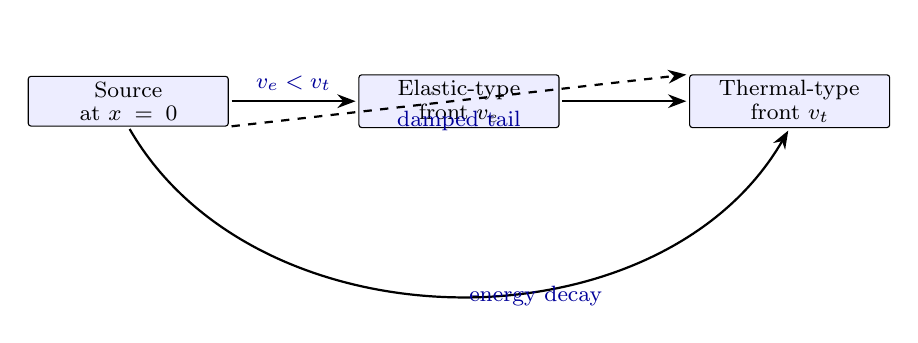
\begin{tikzpicture}[x=1.0cm,y=1.0cm,>=Stealth]
  \tikzset{
    node/.style={draw,rounded corners=1pt,fill=blue!7,align=center,font=\footnotesize,inner sep=2pt,text width=2.4cm},
    arr/.style={->,thick,shorten >=1pt,shorten <=1pt},
    lbl/.style={font=\footnotesize,text=blue!60!black},
  }
  \node[node] at (-3.6, 0.0) (src) {Source\\[-1pt] at $x=0$};
  \node[node] at ( 0.6, 0.0) (fe) {Elastic-type\\[-1pt] front $v_e$};
  \node[node] at ( 4.8, 0.0) (ft) {Thermal-type\\[-1pt] front $v_t$};
  \draw[arr] (src.east) -- (fe.west) node[pos=0.5,above,lbl] {$v_e<v_t$};
  \draw[arr] (fe.east) -- (ft.west) node[pos=0.5,above,lbl] {};
  \draw[arr,dashed] (src.south east) -- (ft.north west) node[pos=0.5,below,lbl] {damped tail};
  \draw[arr] (src.south) to[out=-60,in=240] node[pos=0.5,right,lbl] {energy decay} (ft.south);
\end{tikzpicture}

\caption{Geometry after \citep{Lord1967}: two wave fronts in hyperbolic thermoelasticity -- elastic-type and thermal-type fronts repel in speed; the thermal front carries a damped tail.}\label{fig:fronts}
\end{figure}

\paragraph{Discontinuities and well-posedness.} Because the system is hyperbolic, initial data with a jump produce solutions with jumps carried along the fronts, and these jumps decay exponentially along the propagation path; this is visible in the heat-pulse problem of Section~\ref{sec:transient}. The system is well posed for $\tau_0>0$ and energy decays in bounded bodies under standard boundary conditions, from the energy identity \eqref{eq:energy}. Existence of generalized solutions for one-relaxation-time thermoelasticity was established by \citep{Bem1982}, and for two relaxation times by \citep{Bem1983}; domain-of-influence results appear in \citep{Ignaczak1980}. The thermodynamic foundation via the Clausius--Duhem inequality is due to \citep{GurtinWilliams1966}.

\paragraph{Interpretation.} The principal modelling questions are the physical size of $\tau_0$ and whether Cattaneo's law, with a single exponential relaxation, is an adequate description in the frequency range of interest. Joseph and Preziosi \citep{Joseph1989,Joseph1990} review evidence for and against; large relaxation times have been reported for nonhomogeneous materials \citep{Kaminski1990,Mitra1995}, although the interpretation of such measurements has been debated. For solids the strongest evidence of wave-like heat propagation is second sound at cryogenic temperatures \citep{Ackerman1966,Jackson1970}, where the governing regime is the Guyer--Krumhansl hydrodynamic one \citep{GuyerKrumhansl1966II}, not the simple Cattaneo law.

\subsection{Green--Lindsay theory}\label{sec:gl}
The Green--Lindsay (GL) theory \citep{Green1972} has the constitutive relations
\begin{equation}
\sigma_{ij}=C_{ijkl}\varepsilon_{kl}-\beta_{ij}\bigl(\theta+\tau_1\dot\theta\bigr),\qquad
k\theta_{,ii}=\rho c\bigl(\dot\theta+\tau_0\ddot\theta\bigr)+T_0\beta_{ij}\dot\varepsilon_{ij},\label{eq:GL}
\end{equation}
with $\tau_0\ge\tau_1\ge0$. The heat conduction term is Fourier's, so the theory does not fit the flux template \eqref{eq:template}; the finite thermal speed instead comes from the inertia term $\tau_0\ddot\theta$. Substituting in plane waves gives \eqref{eq:unified} with $\tau^\dagger=\tau_1$. Three differences from LS are worth noting. First, the thermal equation is not of Cattaneo type, so the relation to kinetic arguments is less direct. Second, the entropy is a function of temperature rate, so it is the thermal displacement-like quantity that appears in the constitutive structure, and the interpretation of $\tau_0$ and $\tau_1$ as independent material constants requires care. Third, solutions of the original theory can contain discontinuities that some authors consider unphysical; a modification with a strain-rate term was proposed to remove them \citep{Yu2018ModifiedGL}. Wave fronts follow \eqref{eq:fronts} with $\tau^\dagger=\tau_1$. A distinguishing consequence: in GL the coupling is weaker at the wave fronts than in LS by the factor $\tau_1/\tau_0\le1$.

\subsection{Green--Naghdi types I, II and III}\label{sec:gn}
The Green--Naghdi (GN) theories \citep{Green1991,GreenGN1992,Green1993} postulate an entropy balance with the thermal displacement $v$ ($\dot v=\theta$) as a primary field. In the template the three types are
\begin{equation}
\text{I: }\ q_i=-k\theta_{,i};\qquad
\text{II: }\ q_i=-k^*v_{,i};\qquad
\text{III: }\ q_i=-k\theta_{,i}-k^*v_{,i},
\end{equation}
with $G=k$, $k^*/s$ and $k+k^*/s$, respectively. Their uncoupled thermal equations are, with $\rho c=1$ for brevity,
\begin{equation}
\text{II: }\ \ddot\theta=c_*^2\nabla^2\theta,\quad c_*^2=k^*/\rho c;\qquad
\text{III: }\ \ddot\theta=c_*^2\nabla^2\theta+\alpha\nabla^2\dot\theta.
\end{equation}
\paragraph{Type II.} Thermal disturbances propagate as undamped waves of speed $c_*$, and with coupling the two fronts satisfy \eqref{eq:fronts} with $c_T\to c_*$, $\tau^\dagger/\tau_0\to1$. In this case, however, the relation is \emph{exact for all frequencies}, not only asymptotically: the roots of the quadratic \eqref{eq:disp} with $G=k^*/s$ are non-dispersive, with $v^4-v^2[c_1^2(1+\varepsilon)+c_*^2]+c_1^2c_*^2=0$ at every $\omega$. We confirmed this numerically for $\varepsilon=0.1$ and $c_*=c_1$: the exact speeds $0.854309c_1$ and $1.170537c_1$ are the same at $\omega/\omega_*=0.5$, $2$ and $10$, and agree with the formula. The theory is energy-conserving, so there is no thermoelastic damping at all; it is the only member of the family with this property, and consequently the benchmark for energy-based checks.
\paragraph{Type III.} The type III equation is a damped wave equation with a Kelvin--Voigt-type damping term $\alpha\nabla^2\dot\theta$. Two consequences deserve emphasis. At \emph{low} frequency $G\simeq k^*/s$ and the thermal branch has the type-II speed $c_*$, whereas at \emph{high} frequency $G\to k$ and the branch becomes diffusive: its phase speed is unbounded (\Cref{fig:family}, magenta curve), exactly as in the classical theory. Thus, in contrast to LS, type III is wave-like at low frequencies and diffusive at high frequencies, and its thermal signals do not have a finite propagation speed in the strict sense (the strongly damped wave equation has a parabolic smoothing effect). The practical interpretation is that type III describes weakly damped thermal waves at moderate frequencies; it is not an ``improved Cattaneo law''. Statements in the literature that type III possesses finite thermal wave speed should be read as referring to the undamped limit.
\paragraph{Uniqueness and stability.} Chandrasekharaiah proved uniqueness for type II \citep{Chandrasekharaiah1996}; complete solutions for type II were given by \citep{Chandrasekharaiah1997}; the theory without energy dissipation for anisotropic and micropolar media was developed in \citep{Iesan1998,Quintanilla1999,Ciarletta1999,Quintanilla2002}. Stability and decay results for type III are part of the mathematical theory of thermoelasticity \citep{Suh1998}. The type II theory has attracted attention as a conservative reference model; combined with nonlocal elasticity it has been analysed for wave dispersion \citep{Sarkar2019}.

\begin{summarybox}[Summary]
LS, GL and GN share one dispersion equation \eqref{eq:unified}; they differ in which coupling term carries a time-derivative correction. LS has finite thermal speed $c_T$ from flux relaxation; GL has it from thermal inertia $\tau_0\ddot\theta$; GN-II is non-dispersive and energy-conserving; GN-III is wave-like at low frequency but diffusive at high frequency and has no finite front speed in the strict sense. Front speeds obey \eqref{eq:fronts} and repel when $c_T\approx c_1$.
\end{summarybox}

\section{Lagging and third-order models: DPL, TPL and MGT}\label{sec:lags}
\subsection{The lag idea and its Taylor truncations}
The dual-phase-lag (DPL) model \citep{Tzou1995,Tzou1997} states that the temperature gradient at time $t+\tau_T$ drives the heat flux at time $t+\tau_q$:
\begin{equation}
q_i(\bx,t+\tau_q)=-k\,\theta_{,i}(\bx,t+\tau_T).\label{eq:lag}
\end{equation}
To obtain a differential equation, both sides are expanded in Taylor series. The truncation order is a modelling decision, not a detail, and three variants are in use:
\begin{align}
\text{(i) first order in both:}\quad & q_i+\tau_q\dot q_i=-k\bigl(\theta_{,i}+\tau_T\dot\theta_{,i}\bigr),\label{eq:dpl1}\\
\text{(ii) second order in }\tau_q\text{, first in }\tau_T:\quad & q_i+\tau_q\dot q_i+\tfrac12\tau_q^2\ddot q_i=-k\bigl(\theta_{,i}+\tau_T\dot\theta_{,i}\bigr),\label{eq:dpl2}\\
\text{(iii) second order in both:}\quad & q_i+\tau_q\dot q_i+\tfrac12\tau_q^2\ddot q_i=-k\bigl(\theta_{,i}+\tau_T\dot\theta_{,i}+\tfrac12\tau_T^2\ddot\theta_{,i}\bigr).\label{eq:dpl3}
\end{align}
Version (i) is the member of the template of Section~\ref{sec:framework-link}. Versions (ii) and (iii) have higher-order $G(s)$: for (ii), $G(s)=k(1+\tau_Ts)/(1+\tau_qs+\tau_q^2s^2/2)$.

\paragraph{Why the truncation order matters for stability.} The stability condition $\tau_T\ge\tau_q/2$, often quoted as \emph{the} stability condition of DPL thermoelasticity, was derived by Quintanilla \citep{Quintanilla2003DPL} for the version in which the flux is expanded to second order in $\tau_q$ and the gradient to first order in $\tau_T$, i.e.\ variant (ii). Related stability results for the same model appear in \citep{Quintanilla2002b,Quintanilla2006,Fabrizio2014,Rukolaine2014}. We checked this by computing, for the coupled one-dimensional problem with real wavenumber, the largest real part of the temporal roots $s$ of the characteristic polynomial and maximising it over $k$. For the first-order version (i) the largest growth rate is negative for every $\tau_T>0$ tested ($\tau_T/\tau_q$ from $0.05$ to $1.2$, wavenumbers up to $10^3c_1^{-1}\tau_q^{-1}$, $\varepsilon=0.1$); for the second-order version (ii) it is positive when $\tau_T<\tau_q/2$, vanishes at $\tau_T=\tau_q/2$ and is negative above (\Cref{fig:stability}; script \path{fig_stability.py}). The high-wavenumber growth rate saturates, e.g.\ at $\tau_q\,\mathrm{Re}\,s=0.571$ for $\tau_T/\tau_q=0.3$, so the instability is a \emph{mode-independent exponential growth at short wavelengths} --- an ill-posedness of the model, not a slow instability of a few modes.

\begin{figure}[t]\centering
\includegraphics[width=\textwidth]{figs/fig_stability.pdf}
\caption{Temporal growth rate of the coupled one-dimensional DPL problem ($\varepsilon=0.1$, $\tau_q=1$ in units where $c_1=\omega_*=1$). (a) Maximum real part of the temporal roots against wavenumber for the second-order-in-$\tau_q$ truncation \eqref{eq:dpl2}: for $\tau_T/\tau_q<1/2$ the growth rate tends to a positive constant at large $k$; for $\tau_T/\tau_q\ge1/2$ it is non-positive. (b) The supremum over $k$ against $\tau_T/\tau_q$ for the two truncations; the first-order version \eqref{eq:dpl1} (blue) has no instability.}\label{fig:stability}
\end{figure}

The consequence for the literature is practical. Papers that use the first-order version and state that they ``impose'' $\tau_T\ge\tau_q/2$ for stability are applying a condition that belongs to another model; conversely, papers that use the second-order version with $\tau_T<\tau_q/2$ are computing solutions of an ill-posed problem, and any numerical result is then dominated by the growing high-wavenumber modes. The thermodynamic and continuous-dependence analyses of the time-differential lag models \citep{Chirita2016,Tibullo2017} and modal comparisons with Fourier and Cattaneo laws \citep{vanDerMerwe2021} address the same issue from a different angle. Note also that first-order truncation is valid only when $\tau_q$ and $\tau_T$ are small compared with the time scale of the phenomenon ($\omega\tau\ll1$), a condition that is not satisfied in the frequency range where the lag models are claimed to differ from Fourier's law; we return to this in Section~\ref{sec:synthesis}.

\subsection{Dispersion and the shape of the lag response}
For version (i), $G(s)=k(1+\tau_Ts)/(1+\tau_qs)$ has two limits, $G(0)=k$ and $G(\infty)=k\tau_T/\tau_q$. The thermal branch is therefore diffusive at both ends, with effective diffusivities $\alpha$ at low and $\alpha\tau_T/\tau_q$ at high frequency, and wave-like only at intermediate frequency if $\tau_T<\tau_q$ (\Cref{fig:family}). The statement that ``$\tau_T<\tau_q$ means wave-like conduction and $\tau_T>\tau_q$ means diffusive conduction'' is therefore correct only in the sense of an intermediate regime. When $\tau_T=\tau_q$, $G(s)\equiv k$ and DPL collapses to Fourier's law, whatever the common value of the lags. When $\tau_T>\tau_q$ the effective conductivity increases with frequency.

\begin{figure}[t]\centering
\includegraphics[width=\textwidth]{figs/fig_thermal_family.pdf}
\caption{Uncoupled thermal branch for the models of the template with $\rho c=1$, $k=1$, $\tau=1$ (and $k^*=0.25$ where relevant): (a) phase speed, (b) attenuation. Fourier and GN-III become diffusive at high frequency (unbounded speed); LS saturates at $c_T$; DPL is diffusive at both ends; MGT is wave-like at both ends, with speed $c_*=\sqrt{k^*/\rho c}$ at low frequency and $c_T=\sqrt{k/\rho c\tau}$ at high frequency; GN-II is non-dispersive.}\label{fig:family}
\end{figure}

\subsection{Three-phase-lag model}
The three-phase-lag (TPL) model of Roy Choudhuri \citep{RoyChoudhuri2007} adds a thermal-displacement term to the DPL law,
\begin{equation}
q_i+\tau_q\dot q_i=-\bigl[k\bigl(\theta_{,i}+\tau_T\dot\theta_{,i}\bigr)+k^*\bigl(v_{,i}+\tau_v\dot v_{,i}\bigr)\bigr],\qquad \dot v=\theta,\label{eq:tpl}
\end{equation}
which is the template. Truncations of the lag equations to higher order, introducing more constants, are common in applications \citep{Abouelregal2020,Abouelregal2020a}. Because TPL includes GN-III as the special case $\tau_q=\tau_T=\tau_v=0$, it inherits the type-III behaviour at low frequency ($G\sim k^*/s$) unless $k^*=0$. For $\tau_q>0$, $G(\infty)=k\tau_T/\tau_q$ (if $\tau_T>0$) so the high-frequency limit is diffusive as in DPL. The thermodynamic compatibility and continuous dependence of the TPL model are studied in \citep{Chirita2016}. For plane waves the nonlocal TPL dispersion was studied in \citep{Tiwari2021}, combinations with memory-dependent derivatives in \citep{Singh2019,Singh2020a,Biswas2019} and with magnetic fields and nonlocal elasticity in \citep{Bayones2021}.

The end effects of three-phase-lag heat conduction were studied by \citep{Quintanilla2008}, with stability conditions given in \citep{Quintanilla2008a}; a well-posed formulation of the three-dual-phase-lag heat conduction equation appears in \citep{Quintanilla2009}. Dual-phase-lag heat conduction and ignition of a solid were analysed by \citep{Antaki2000}, and analytical solutions for nonhomogeneous DPL heat conduction problems were given by \citep{Julius2017}.

\subsection{Moore--Gibson--Thompson thermoelasticity}\label{sec:mgt}
The Moore--Gibson--Thompson (MGT) equation, a third-order-in-time linear model arising in nonlinear acoustics \citep{MooreGibson1960}, has been studied as an abstract evolution equation with memory and in the critical regime \citep{MarchandMcDevittTriggiani2012,LasieckaWang2015MGT,DellOroLasieckaPata2016MGT,DellOroPata2016Viscoelasticity}. Quintanilla \citep{Quintanilla2019} introduced a thermoelastic theory with the flux law
\begin{equation}
\tau\dot q_i+q_i=-k\theta_{,i}-k^*v_{,i},
\end{equation}
which is the Green--Naghdi III law with a relaxation of the flux, i.e.\ the template with $\tau_q=\tau$, $\tau_T=\tau_v=0$. The uncoupled thermal equation is third order in time,
\begin{equation}
\tau\dddot\theta+\ddot\theta=c_*^2\nabla^2\theta+\alpha\nabla^2\dot\theta\ \ (\rho c=1)\,.
\end{equation}
Its structure explains the dispersion shown in \Cref{fig:family}: $G(s)=(k+k^*/s)/(1+\tau s)$ gives $G\simeq k^*/s$ at low frequency (wave speed $c_*$) and $G\simeq k/(\tau s)$ at high frequency (wave speed $c_T=\sqrt{k/\rho c\tau}$). The model thus has finite signal speed at high frequency, in contrast to GN-III; and a low-frequency regime with undamped-type thermal waves. The decay of radial solutions of MGT thermoelasticity is analysed in \citep{Bazarra2021MGTradial}. The wave-dispersion questions that remain open include the sign conditions that guarantee decay for the full coupled system with all parameters positive and the behaviour of the thermal front for finite $\tau$; applications to piezo-semiconductors with fractional MGT have appeared \citep{Gupta2024,Aldandani2026}.

\subsection{Hyperbolic two-temperature models}
Two-temperature theories \citep{ChenGurtin1968,Youssef2006} distinguish the conductive temperature $\varphi$ from the dynamic temperature $\theta$, linked by $\theta=\varphi-a\nabla^2\varphi$ with $a\ge0$ a length-squared constant, and hyperbolic versions combine this with LS or GN heat laws \citep{Prasad2020,Alzahrani2020,Bassiouny2020}. In plane waves the two temperatures differ by the factor $1+ak^2$, so a wavenumber dependence enters the dispersion relation through $a$; this plays a role comparable to a nonlocal length scale as regards high-wavenumber behaviour. Stability and characterization of plane waves in the hyperbolic two-temperature theory are in \citep{Prasad2020}.

\subsection{Summary of the template models}
\Cref{tab:compare} compiles the qualitative properties that were verified in Sections~\ref{sec:hyperbolic}--\ref{sec:lags}.
\begin{table}[t]\centering\small
\caption{Properties of the uncoupled thermal branch in the template models (verified from $G(s)$ and by the scripts listed in Appendix~\ref{app:repro}).}\label{tab:compare}
\begin{tabular}{@{}p{3.2cm}p{2.3cm}p{2.3cm}p{2.3cm}p{2.6cm}@{}}\toprule
Model & Low-$\omega$ thermal speed & High-$\omega$ thermal speed & Finite signal speed & Dissipative\\\midrule
Classical & $\propto\sqrt{\omega}$ & $\propto\sqrt{\omega}$ & no & yes\\
Lord--Shulman & $\propto\sqrt{\omega}$ & $\to c_T$ & yes & yes\\
DPL (1st order) & $\propto\sqrt{\omega}$ & $\propto\sqrt{\omega}$ ($\alpha\tau_T/\tau_q$) & no (strict) & yes\\
GN II & $c_*$ & $c_*$ & yes & no\\
GN III & $c_*$ & $\propto\sqrt{\omega}$ & no (strict) & yes\\
TPL ($k^*\neq0$) & $c_*$ & $\propto\sqrt{\omega}$ if $\tau_T>0$ & no (strict) & yes\\
MGT & $c_*$ & $\to c_T$ & yes & yes\\\bottomrule
\end{tabular}
\end{table}
\Cref{tab:compare} gives a more discriminating picture than the common statement ``all generalized theories have finite thermal speed''. A thermal front with finite speed requires that $sG(s)$ tend to a finite nonzero limit as $s\to\infty$ (then $K\simeq-s\rho c/G\propto\omega^2$); this holds for LS, MGT and GN-II and fails for the classical law, DPL, TPL and GN-III in the first-order template.


\begin{summarybox}[Summary]
DPL adds $\tau_T\dot\theta_{,i}$ to Fourier's law; first-order truncation is stable for all positive $\tau_q,\tau_T$ and the widely quoted $\tau_T\ge\tau_q/2$ condition belongs to a specific Taylor truncation, not to the template. TPL adds $\tau_v$; $G(s)\sim k^*/s$ as $s\to0$ for $k^*\ne0$, so low-frequency response differs qualitatively. MGT adds $\tau_R\ddot q_i$ and is third order in time. Finite thermal speed requires $sG(s)\to$ finite nonzero as $s\to\infty$: holds for LS, MGT, GN-II; fails for classical, DPL, TPL, GN-III (first-order template).
\end{summarybox}
\section{Fidelity of Taylor-truncated lag models}\label{sec:delayfid}

\Cref{sec:lags} treats the dual-phase-lag (DPL) law through Taylor truncations of the shifted fluxes. This is a modelling choice, not an identity, and its consequences deserve a quantitative look. Here we compare the truncations with the \emph{exact} delay law on the uncoupled thermal branch.

\subsection{Setting}
Take $\tau_T=0$ in the DPL law, $q(t+\tau_q)=-k\,\theta_{,x}(t)$. In the Laplace/Fourier representation the exact delay gives $G(s)=k\,e^{-\tau_q s}$, the first-order truncation gives $G=k/(1+\tau_q s)$ (Cattaneo), and the second-order truncation gives $G=k/(1+\tau_q s+\tau_q^2s^2/2)$. With $s=-i\omega$ the thermal branch satisfies $k_w^2=-\rho c\,s/G(s)$, where $k_w$ is the wavenumber. All three differ only through $G$, so they coincide as $\omega\tau_q\to0$.

\subsection{Numerical comparison}
\Cref{fig:lagtrunc} shows phase speed and attenuation for the three laws, computed by \path{scripts/fig_lag_truncation.py}. The relative error in $k_w$ against the exact delay is
\begin{center}
\begin{tabular}{@{}lcccc@{}}
\toprule
$\omega\tau_q$ & 0.05 & 0.1 & 0.3 & 1.0\\
\midrule
first order & $6\times10^{-4}$ & $2.5\times10^{-3}$ & $2.2\times10^{-2}$ & $0.22$\\
second order & $1\times10^{-5}$ & $8\times10^{-5}$ & $2.2\times10^{-3}$ & $0.08$\\
\bottomrule
\end{tabular}
\end{center}
Both truncations are accurate for $\omega\tau_q\lesssim0.3$ and lose accuracy at $\omega\tau_q\sim1$, which is exactly where lagging effects are claimed to matter. Conclusions drawn at $\omega\tau_q\gtrsim1$ from a truncated law therefore describe the truncated model, not the delay law.

\begin{figure}[t]
\centering
\includegraphics[width=\linewidth]{figs/fig_lag_truncation.pdf}
\caption{Thermal branch for the exact delay $e^{-\tau s}$, first-order and second-order truncations: (a) speed, (b) attenuation. Roots are taken with $\operatorname{Im}k\ge0$, so the real part of $k$ of the delay law can be negative at higher $\omega\tau$ and the spikes of $|v_p|$ mark zeros of $\operatorname{Re}k$. The dotted line marks $\omega\tau=\pi/2$, where the attenuation of the principal root of the delay law changes sign.}
\label{fig:lagtrunc}
\end{figure}

\subsection{Sign change of attenuation in the exact delay law}
For the exact delay the principal root is $k_w=\sqrt{\rho c\,\omega/k}\;e^{i(\pi/4-\omega\tau_q/2)}$, so $\operatorname{Im}k_w<0$ once $\omega\tau_q>\pi/2$ (numerically checked: $\operatorname{Im}k_w>0$ at $\omega\tau_q=1$, $=0$ at $\pi/2$, $<0$ at $2$). Choosing $\operatorname{Re}k_w>0$ then gives spatial growth, and choosing decay gives a negative phase speed. The truncations avoid this behaviour, but only because they discard the high-frequency part of the delay. This is a reason for caution when a delay law is used beyond $\omega\tau_q\approx\pi/2$ and a reason to state, in any application, which truncation is used.

\subsection{Practical rule}
(i) Report the truncation order together with $\tau_q,\tau_T$. (ii) Check $\omega\tau_q\lesssim0.3$ before trusting a truncated law as an approximation of the delay law. (iii) Do not read agreement between two truncated laws at $\omega\tau_q\sim1$ as confirmation of the delay model.


\begin{summarybox}[Summary]
The exact delay law $\tau_q\dot q(t)+q(t)=-k\theta_{,i}(t-\tau_T)$ has infinitely many branches because $G(s)$ contains an exponential. Taylor truncation replaces it by a rational function with finitely many roots. Truncated and exact laws agree only for $\omega\tau_q\lesssim0.3$; above that, spurious and missing roots make the truncation unreliable. Always report the truncation order together with the lag values.
\end{summarybox}
\section{Fractional and memory-dependent models}\label{sec:memory}
\subsection{Motivation}
Fractional and memory-dependent derivatives replace the local-in-time structure of Cattaneo's and Tzou's laws by an operator that weights the past, so that the response at time $t$ depends on the history of the gradient or flux. Three motivations are cited: anomalous (sub- or super-diffusive) heat transport in heterogeneous and porous media, relaxation spectra that are not single-exponential, and the wish to interpolate between diffusive and wave-like conduction with a single parameter.

\subsection{Caputo-fractional heat conduction}
The Caputo derivative of order $\alpha>0$ with $m-1<\alpha\le m$, $m$ integer, is \citep{Caputo1967,Podlubny1999}
\begin{equation}
{}^C\!D^\alpha f(t)=\frac1{\Gamma(m-\alpha)}\int_0^t(t-\xi)^{m-\alpha-1}f^{(m)}(\xi)\,\dd\xi,\qquad
\mathcal L\{{}^C\!D^\alpha f\}=s^\alpha\hat f-\sum_{j=0}^{m-1}s^{\alpha-1-j}f^{(j)}(0).\label{eq:caputo}
\end{equation}
The Laplace rule in \eqref{eq:caputo} is the reason for the Caputo definition: initial conditions have their usual physical meaning. Two families of fractional heat-conduction models are in common use.
\begin{enumerate}
\item \emph{Time-fractional heat equation} \citep{Povstenko2004,Povstenko2007,Povstenko2009}: $\rho c\,{}^C\!D^\alpha\theta=k\nabla^2\theta$ with $0<\alpha\le2$, interpolating between the diffusion ($\alpha=1$) and a wave-like ($\alpha=2$) equation, with subdiffusion for $\alpha<1$ and diffusion--wave behaviour for $1<\alpha<2$.
\item \emph{Fractional Cattaneo-type law} \citep{Povstenko2011Cattaneo,Sherief2010Fractional,Ezzat2011}: $q_i+\tau^\alpha\,{}^C\!D^\alpha q_i=-k\theta_{,i}$, with $G(s)=k/(1+(\tau s)^\alpha)$ in the Laplace domain.
\end{enumerate}
Further variants (fractional DPL and TPL, with fractional orders on one or both sides of the lag equation) are numerous; reviews and critical discussions of the logic of fractional thermoelasticity are given in \citep{Povstenko2016,Yu2024,Gorenflo1997,Povstenko2004,Povstenko2007,Povstenko2009}.

\paragraph{The diffusion--wave equation.} For the first family and prescribed boundary temperature $\theta_0$ on the half-line $x>0$, with zero initial data, the Laplace-domain solution is $\hat\theta=(\theta_0/s)\exp(-x\,s^{\alpha/2}/\sqrt{a})$, $a=k/\rho c$ (with a fractional time scale absorbed in $a$). For $\alpha=1$ this inverts to $\theta_0\,\mathrm{erfc}(x/2\sqrt{at})$, which we reproduced numerically with Talbot inversion to eight digits ($0.4795001$ at $x/\sqrt{at}=1$). For $\alpha=2$ it gives the step $\theta_0H(t-x/\sqrt a)$, a pure wave with no dispersion or damping; for $\alpha<1$ the solution is a stretched Mittag-Leffler-type decay with heavy tails \citep{GorenfloKilbasMainardiRogosin2014,Luchko2010}. \Cref{fig:fractional}(a) displays the family. Two cautions: (i) the endpoint $\alpha=2$ is \emph{not} Fourier's law, but a undamped wave equation, and (ii) for $1<\alpha<2$ the equation requires two initial conditions, one of which ($\dot\theta(0)=0$) is chosen by convention.

\subsection{Memory-dependent derivative}
The memory-dependent derivative (MDD) of Wang and Li \citep{Wang2011} is defined for a delay (memory) window $\tau>0$ by
\begin{equation}
D_\tau f(t)=\frac1\tau\int_{t-\tau}^{t}K(t-\xi)\,f'(\xi)\,\dd\xi,\qquad K(u)=1-\frac{2b\,u}{\tau}+\frac{a\,u^2}{\tau^2},\label{eq:mdd}
\end{equation}
with $a,b$ constants; the choices $a=b=1$ ($K=(1-u/\tau)^2$), $a=0,b=\tfrac12$ ($K=1-u/\tau$) and $a=b=0$ ($K=1$) are popular (\Cref{fig:fractional}b). The operator differs from the fractional derivative in having a finite window, a bounded kernel, and a clear time-domain meaning as a weighted average of the rate over the last $\tau$ time units; Wang and Li's comparison with the fractional derivative \citep{Wang2021,WangLi2025IV} discusses the relation of the two. MDD versions of lag models replace the first-order derivatives in \eqref{eq:dpl1} or \eqref{eq:tpl} by $D_\tau$ \citep{Singh2019,Singh2020a,Biswas2019,Abouelregal2023,Sur2019,Sur2025,Hamza2014,Sur2012,Yu2014,Sherief2018,Ezzat2015}.

\paragraph{Laplace transform of the MDD.} Because $f'$ vanishes for negative arguments, \eqref{eq:mdd} is a convolution of $f'$ with $K(u)\mathbf 1_{[0,\tau]}(u)/\tau$, and
\begin{equation}
\mathcal L\{D_\tau f\}=s\,\kappa(s)\,\hat f,\qquad \kappa(s)=\frac1\tau\int_0^\tau K(u)\,e^{-su}\,\dd u.\label{eq:kappa}
\end{equation}
For the kernel $K=(1-u/\tau)^2$, $\kappa(0)=\tfrac13$ and $s\kappa(s)\to K(0)/\tau=1/\tau$ as $s\to\infty$. An MDD version of Cattaneo's law, $q_i+\tau D_\tau q_i=-k\theta_{,i}$, therefore has $G(s)=k/\bigl(1+\tau s\kappa(s)\bigr)$, which tends to $k/2$ (not to zero!) at high frequency: the thermal branch of this particular MDD-Cattaneo law becomes \emph{diffusive} at high frequency with half the low-frequency diffusivity, in contrast to the ordinary Cattaneo law, for which $G\to0$ and the speed saturates (\Cref{fig:fractional}c, green dashed curve versus blue). The reason is that a bounded kernel with $K(0)=1$ gives $\tau D_\tau\to$ a time-local multiple of the identity at high frequency, which acts as a constant added to the denominator rather than a derivative. This is a model-specific property: a kernel with $K(0)=0$ would give $\tau s\kappa(s)\to0$ and hence $G\to k$ (Fourier behaviour) at high frequency, and other MDD formulations of the lag laws behave differently, so the consequence for wave fronts must be checked for the variant at hand.

\begin{figure}[t]\centering
\includegraphics[width=\textwidth]{figs/fig_fractional_mdd.pdf}
\caption{(a) Caputo time-fractional heat equation, boundary temperature step, profiles at $t=t_0$ for $\alpha=0.5,1,1.5,2$ (Talbot inversion; the case $\alpha=2$ is the exact step front). (b) Kernels of the memory-dependent derivative \eqref{eq:mdd}. (c) Phase speed of the uncoupled thermal branch for Fourier, Cattaneo, fractional Cattaneo with $\alpha=0.8$ and MDD-Cattaneo ($a=b=1$), normalised by the Cattaneo wave speed.}\label{fig:fractional}
\end{figure}

Memory-dependent derivative modelling was introduced by \citep{Wang2011}; MDD-based generalized thermoelasticity was developed by \citep{Ezzat2016}, electro-thermoelasticity with MDD heat transfer by \citep{Ezzat2016a}, and DPL thermoelasticity with MDD by \citep{Ezzat2016b}. Time-fractional radial heat conduction in a sphere was treated by \citep{Povstenko2011}; the view of thermoelasticity and generalized thermoelasticity as wave hierarchies was presented by \citep{Scott2007}; a theory of generalized thermoelasticity with memory-dependent derivatives was given by \citep{Shaw2019}. The time-fractional dual-phase-lag heat conduction equation was formulated by \citep{Xu2015}; fractional order generalized thermoelasticity was developed by \citep{Youssef2010} with its variational principle in \citep{Youssef2010a}; and fractional order theory of Cattaneo-type thermoelasticity using new fractional derivatives was introduced by \citep{Yu2020}.

\subsection{Position of these models in the template}
Because $G(s)$ for fractional and MDD models is not rational, the dispersion relation \eqref{eq:disp} is still quadratic in $K$ with $G(s)$ evaluated at complex $s=-\ii\omega$ (with principal branches), so that the analysis of Section~\ref{sec:longitudinal} carries over verbatim; only the closed-form front-speed analysis and the transform inversion change. The energy functionals, uniqueness and thermodynamic admissibility of these models are less developed than for the template models, and their thermodynamic admissibility has been discussed with differing conclusions. A practical concern is that the extra order or memory parameter can be tuned to fit a single dataset without independent confirmation. The reinterpretation of fractional thermoelasticity in terms of anomalous heat conduction \citep{Yu2024} and the thermodynamic consistency analyses of time-differential lag models \citep{Chirita2016,Tibullo2017} provide the context in which one should choose among them.

\begin{summarybox}[Summary]
Fractional (Caputo) and memory-dependent derivative laws replace $s$ in $G(s)$ by non-integer powers or kernel transforms, so the dispersion relation stays quadratic in $K$ but roots are complex and front analysis changes. Thermodynamic admissibility, energy functionals and uniqueness are less developed than for the template models. The extra parameter can be fitted to one dataset without independent confirmation---a fitting constant is not a material property.
\end{summarybox}

\section{Coupled fractional dispersion}\label{sec:fraccoupled}

The memory models of \cref{sec:memory} are usually analysed on the heat equation alone. Here we put a fractional Cattaneo law, $q+\tau^{\alpha}D^{\alpha}q=-k\,\theta_{,x}$ with a Caputo derivative $D^\alpha$ and $0<\alpha\le1$, into the coupled longitudinal problem of \cref{sec:classical}. In the Laplace representation $G(s)=k/[1+(\tau s)^{\alpha}]$, and the polynomial of \cref{eq:unified} is used unchanged, with the principal branch $(-i\omega)^\alpha=\omega^\alpha e^{-i\pi\alpha/2}$.

\Cref{fig:fraccoupled} (script \path{scripts/fig_frac_coupled.py}) shows phase speed and loss for the elastic-like branch, tracked by continuity in $\omega$, for $\varepsilon=0.1$, $\tau\omega^*=0.25$ (so that the thermal front speed is twice $c_1$ and the branches do not hybridise degenerately). The numbers that can be read from it are:
\begin{itemize}
\item At low frequency all models give the adiabatic speed $c_1\sqrt{1+\varepsilon}=1.0488\,c_1$.
\item The classical Debye peak is $Q^{-1}=0.0501\approx\varepsilon/2$ at $\omega/\omega^*\approx1.1$.
\item The lagging and fractional models shift and raise the peak: $0.0701$ at $\omega/\omega^*=1.42$ for $\alpha=1$, $0.0741$ at $1.58$ for $\alpha=0.8$ and $0.0728$ at $1.75$ for $\alpha=0.6$.
\item At the top of the plotted range $v_p/c_1=0.984,\,0.993,\,0.997$ for $\alpha=1,\,0.8,\,0.6$, and $1.000$ for the classical model.
\end{itemize}
The qualitative message is that the fractional order moves the position and height of the loss peak by amounts comparable to the Cattaneo--classical difference, so it cannot be treated as a small correction. These numbers belong to this parameter set; a different $\tau\omega^*$ changes them, and the figure should be reproduced for the material at hand.

\begin{figure}[t]
\centering
\includegraphics[width=\linewidth]{figs/fig_frac_coupled.pdf}
\caption{Coupled longitudinal wave with a fractional Cattaneo law: (a) phase speed, (b) loss $Q^{-1}$ for $\alpha=1,0.8,0.6$ and the classical model ($\varepsilon=0.1$, $\tau\omega^*=0.25$).}
\label{fig:fraccoupled}
\end{figure}

\begin{summarybox}[Summary]
For fractional Cattaneo conduction $G(s)=k/(1+\tau s^\alpha)$, the dispersion polynomial \eqref{eq:disp} still applies with complex $s$. The endpoint $\alpha\to2$ is second order in time, not Fourier's law; $\alpha\to1$ gives Cattaneo. Phase speed and loss interpolate between classical ($lpha=1$) and increasingly wave-like behaviour as $lpha$ decreases, with no sharp front unless a finite-speed kernel is used.
\end{summarybox}

\section{Wave propagation in three dimensions}\label{sec:waves3d}
\subsection{Plane waves in an isotropic generalized thermoelastic solid}
In an unbounded isotropic solid with any heat-flux law of the template, \eqref{eq:helm} generalises to
\begin{equation}
\rho\ddot\phi=(\lambda+2\mu)\nabla^2\phi-\beta\theta,\quad
s\rho c\,\hat\theta+T_0\beta s\nabla^2\hat\phi=G(s)\nabla^2\hat\theta,\quad
\rho\ddot{\bm\psi}=\mu\nabla^2\bm\psi,
\end{equation}
and a plane wave in direction $\bm n$, $\propto\exp[\ii(k\,\bm n\!\cdot\!\bx-\omega t)]$, has the same characteristic equation \eqref{eq:disp} for the dilatational--thermal system. The dispersion analysis of Section~\ref{sec:longitudinal} therefore applies without change to waves in any direction of an isotropic body. The shear wave has speed $c_2$ and is not affected by the heat-flux law, for any member of the template and for fractional or memory models as well. For general anisotropy the quasi-longitudinal, quasi-shear and thermal branches couple through $\beta_{ij}$ and $k_{ij}$, and the characteristic equation becomes a polynomial of higher degree; Dhaliwal and Sherief's formulation \citep{Dhaliwal1980} is the standard reference, and for numerical dispersion the Stroh formalism \citep{Stroh1958,Stroh1962} is convenient.

\paragraph{Counting branches.} The number of branches in a bulk plane-wave problem is $2$ (dilatational--thermal) $+\,2$ (shear polarisations) in an isotropic medium, with $G$ rational of low degree; the degree of the polynomial in $K$ equals $2$ only if $G$ is rational of the kind in the template. For the second-order lag version (ii) \eqref{eq:dpl2}, or higher-order models, the number of thermal-type branches increases. Several additional branches appear in published dispersion curves of such models, and it is advisable to separate genuine physical branches from spurious roots created by Taylor truncation.

\subsection{Reflection at a free surface: structure of the problem}
A plane dilatational wave incident on a plane free surface in an isotropic thermoelastic half-space generates reflected waves of three kinds: a dilatational (elastic-type) wave, a thermal-type wave (evanescent or strongly damped), and a shear (SV) wave. Boundary conditions are the traction-free conditions together with a thermal condition, either \emph{insulated} (zero normal flux, $\partial_n\theta=0$ for any $G$) or \emph{isothermal} ($\theta=0$). The amplitude ratios are obtained from a $3\times3$ linear system and have been computed for many models; the comparison of insulated and isothermal boundaries for generalized theories is a classical exercise \citep{Das2008}, and extensions with nonlocal, micropolar, piezoelectric and rotational effects are numerous \citep{Kalkal2020,Singh2020b,Yadav2023,Gupta2024a}. We will not tabulate their results; instead, Section~\ref{sec:surface} gives the structure of the free-surface problem used for Rayleigh waves, which is the same determinant, and Section~\ref{sec:interfaces} treats the interface problem with a verified energy check.

\begin{figure}[t!]\centering\small
% fig4_reflection.tex -- Half-space reflection geometry (s08_waves3d)
\begin{tikzpicture}[x=1.0cm,y=1.0cm,>=Stealth]
  \tikzset{
    node/.style={draw,rounded corners=1pt,fill=blue!7,align=center,font=\footnotesize,inner sep=2pt,text width=2.2cm},
    arr/.style={->,thick,shorten >=1pt,shorten <=1pt},
    lbl/.style={font=\footnotesize,text=blue!60!black},
    medium/.style={fill=blue!10},
    surfaceline/.style={thick},
  }
  % Half-space region y>0 shaded
  \fill[medium] (-3.5,0) -- (3.5,0) -- (3.5,3.5) -- (-3.5,3.5) -- cycle;
  % Free surface line
  \draw[surfaceline] (-3.5,0) -- (3.5,0);
  \node[below=2pt] at (0,0) {free surface $y=0$};
  % Axes
  \draw[->,thick] (-3.5,0) -- (3.5,0) node[right] {$x$};
  \draw[->,thick] (0,0) -- (0,3.5) node[above] {$y$};
  % Incident P wave from upper left
  \draw[arr,very thick] (-2.5,2.0) -- (-0.7,0.6);
  \node[above left,lbl] at (-2.5,2.0) {incident P};
  % Reflected P wave
  \draw[arr,very thick] (-0.7,0.6) -- (1.5,2.2);
  \node[above right,lbl] at (1.5,2.2) {reflected P};
  % Reflected SV wave
  \draw[arr,very thick] (-0.7,0.6) -- (1.5,-0.8);
  \node[below right,lbl] at (1.5,-0.8) {reflected SV};
  % Thermal-type (evanescent) wave going down
  \draw[arr,dashed,very thick] (-0.7,0.6) -- (0.5,-2.0);
  \node[below,lbl] at (0.5,-2.0) {thermal (evanescent)};
  % Region label
  \node[above] at (0,3.2) {half-space $y>0$};
  % Boundary condition labels
  \node[below=6pt,align=center] at (-1.2,0) {insulated\\(\\partial_n\\theta=0)\\\\\nor isothermal\\($\\theta=0$)};
\end{tikzpicture}

\caption{Geometry after \citep{Das2008}: reflection at a free thermoelastic surface -- an incident P wave generates reflected P, reflected SV and a thermal-type (evanescent/damped) wave; thermal condition insulated or isothermal.}\label{fig:reflection-geo}
\end{figure}

\subsection{Waves in plates, rods and layered structures}
In bounded waveguides, the thermal and elastic fields are coupled by lateral boundary conditions and a family of guided modes arises (Lamb modes in plates \citep{Lamb1917}, Pochhammer--Chree modes in rods). The thermoelastic version has one additional family of thermal modes per thermal condition, and the dispersion curves of the elastic modes are perturbed by the thermal coupling in the same way as in \Cref{fig:disp}: small speed corrections and a damping that peaks where the thermal relaxation frequency of the cross-section matches the wave frequency. For thin plates and beams the flexural damping reduces to Zener's classical result (Section~\ref{sec:ted}). Texts on the elastic waveguide problem are \citep{Achenbach1973,Auld1973}; for the thermoelastic waveguide with generalized laws the literature consists mainly of analyses of specific configurations \citep{Biswas2020,Abouelregal2023}.

\begin{summarybox}[Summary]
In an unbounded isotropic body plane waves split into a shear branch (speed $c_2$, unaffected by heat) and a coupled dilatational--thermal system governed by \eqref{eq:disp}. Reflection at a free surface generates three reflected waves (P, SV, thermal-type), with amplitude ratios from a $3\times3$ system. In waveguides each thermal condition adds a family of thermal modes.
\end{summarybox}

\section{Anisotropy: thermal coupling of quasi-longitudinal waves in cubic crystals}\label{sec:aniso}

Most of the theory above is isotropic. Real devices use single crystals, and the question is how the coupling strength $\varepsilon$ depends on the propagation direction and which modes are affected.

\subsection{Christoffel problem with thermal coupling}
For a cubic crystal the thermal expansion is isotropic, $\alpha_{ij}=\alpha_T\delta_{ij}$, so the thermal-stress tensor is $\beta_{ij}=\beta_0\delta_{ij}$ with $\beta_0=(c_{11}+2c_{12})\alpha_T$, and heat conduction is scalar. For a plane wave with direction $\bm n$ the field equations give, in the low-frequency (adiabatic) limit $\omega\ll\omega_*$, the Christoffel equation
\begin{equation}\label{eq:christ}
\bigl[\Gamma_{ik}(\bm n)+\tfrac{\beta_0^2T_0}{c_v}\,n_in_k-\rho v^2\delta_{ik}\bigr]p_k=0,\qquad \Gamma_{ik}=C_{ijkl}n_jn_l,
\end{equation}
where $c_v$ is the volumetric heat capacity, and in the high-frequency (isothermal) limit the same equation without the thermal term. The thermal term is a rank-one matrix along $\bm n$, so it couples only to the polarisation component along the propagation direction, and it vanishes for purely transverse modes. Along the symmetry directions of a cubic crystal the coupling is therefore governed by
\begin{equation}\label{eq:epsdir}
\varepsilon_{\bm n}=\frac{\beta_0^2T_0}{c_v\,M_{\bm n}},\qquad M_{[100]}=c_{11},\ M_{[110]}=\tfrac12(c_{11}+c_{12}+2c_{44}),\ M_{[111]}=\tfrac13(c_{11}+2c_{12}+4c_{44}),
\end{equation}
with $M_{\bm n}$ the longitudinal modulus along $\bm n$, and the quasi-longitudinal speed rises from the isothermal to the adiabatic value by the factor $\sqrt{1+\varepsilon_{\bm n}}$. Both transverse modes along these directions are unaffected.

\subsection{Numerical values}
\Cref{tab:aniso} gives the result for three cubic metals and semiconductors, computed with the script \path{scripts/fig_aniso.py} from rounded handbook values of the elastic constants, expansion coefficient, density and specific heat at $T_0=300$\,K; these inputs should be replaced by the measurements for a specific sample. The speed shifts obtained from the full eigenvalue problem agree with $\varepsilon_{\bm n}/2$ to the digits shown.

\begin{table}[ht]\centering\small
\caption{Direction dependence of the thermoelastic coupling of quasi-longitudinal waves ($T_0=300$\,K, rounded handbook inputs). $\varepsilon_{\bm n}$ from \cref{eq:epsdir}; shift is $100(v_{\rm ad}/v_{\rm iso}-1)$.}\label{tab:aniso}
\begin{tabular}{@{}lccccc@{}}\toprule
 & \multicolumn{2}{c}{$[100]$} & \multicolumn{2}{c}{$[111]$} & ratio\\
Crystal & $\varepsilon$ & shift (\%) & $\varepsilon$ & shift (\%) & $\varepsilon_{[100]}/\varepsilon_{[111]}$\\\midrule
Cu & 0.0238 & 1.18 & 0.0169 & 0.84 & 1.41\\
Al & 0.0325 & 1.61 & 0.0306 & 1.52 & 1.06\\
Si & $6.5\times10^{-4}$ & 0.032 & $5.3\times10^{-4}$ & 0.026 & 1.23\\
\bottomrule\end{tabular}
\end{table}

For copper the coupling differs by $41\%$ between $[100]$ and $[111]$, so the thermoelastic loss peak height (proportional to $\varepsilon_{\bm n}$ in the weak-coupling Debye form) and the adiabatic--isothermal speed gap are direction dependent by a comparable amount. For aluminium the anisotropy of the coupling is only $6\%$ because the elastic anisotropy is weak, and for silicon the coupling is tiny at all angles, so the longitudinal-wave thermoelastic loss is very small in that material.

\begin{figure}[t]
\centering
\includegraphics[width=\linewidth]{figs/fig_aniso.pdf}
\caption{(a) Adiabatic phase speeds of the three modes of copper in the (001) plane as functions of the propagation angle from $[100]$. (b) Relative stiffening $v_{\rm ad}/v_{\rm iso}-1$ of the quasi-longitudinal mode for Cu, Si and Al.}
\label{fig:aniso}
\end{figure}

\subsection{What changes for the heat-flux law}
Anisotropic heat conduction (non-cubic crystals) makes $G$ a tensor, so the template of \cref{sec:foundations} generalises to $\hat q_i=-G_{ij}(s)\hat\theta_{,j}$ and the lag times may differ along different crystal axes. For the cubic case used here, conduction is isotropic and only the elastic and coupling anisotropy enter, so every scalar result of the preceding sections carries over with $c_1^2\to M_{\bm n}/\rho$ and $\varepsilon\to\varepsilon_{\bm n}$ for propagation along a high-symmetry direction. Away from those directions the quasi-longitudinal polarisation is not along $\bm n$, the coupling is reduced by $(\bm n\!\cdot\!\bm p)^2$, and a quasi-transverse mode acquires a small thermal component.


\begin{summarybox}[Summary]
Anisotropy replaces scalar moduli by tensors $C_{ijkl},\beta_{ij},k_{ij}$; shear and dilatation no longer decouple and the Stroh formalism is the systematic tool. Along high-symmetry directions scalar results carry over with effective moduli. Away from them, quasi-longitudinal and quasi-shear modes mix, coupling weakens by $(\bm n\cdot\bm p)^2$, and quasi-transverse waves acquire a small thermal component.
\end{summarybox}
\section{Reflection at a thermoelastic free surface: numerical results}\label{sec:reflection}

\Cref{sec:waves3d} described the structure of the free-surface problem. Here we give numbers, and a validation, for a plane P wave incident on an insulated traction-free surface of an isotropic thermoelastic half-space.

\subsection{Method}
The half-space is $y>0$ with plane strain and the same non-dimensionalisation as in \cref{sec:surface} ($\rho=c_1=c_v=\omega_*^{-1}=1$, $\nu=0.3$, $\varepsilon=0.1$). The tangential wavenumber $k_x=\operatorname{Re}(k_P)\sin\theta$ is real and conserved. The incident elastic-type wave has amplitude one; the reflected field consists of a P wave, a thermal wave that decays with distance from the surface, and an SV wave, and the three amplitudes follow from the $3\times3$ system of two traction conditions and the insulation condition. The columns of the system are those of the Rayleigh determinant of \cref{sec:surface}, with the sign of the transverse wavenumber reversed for the incident wave (script \path{scripts/fig_reflection.py}).

\subsection{Validation}
For $\varepsilon=10^{-10}$ and $\omega/\omega_*=0.5$ the system reduces to the elastic problem. The computed displacement-amplitude coefficients agree with the classical closed forms for a free surface, 
\begin{equation}
R_{PP}=\frac{\sin2\theta\sin2\phi-\kappa^2\cos^22\phi}{\sin2\theta\sin2\phi+\kappa^2\cos^22\phi},\qquad
R_{PS}=\frac{2\kappa\sin2\theta\cos2\phi}{\sin2\theta\sin2\phi+\kappa^2\cos^22\phi},
\end{equation}
with $\kappa=c_1/c_2$ and $\sin\phi=\kappa^{-1}\sin\theta$, to $1.5\times10^{-10}$ in $|R_{PP}|$ and $8\times10^{-11}$ in $|R_{PS}|$ over $1^\circ\le\theta\le70^\circ$ (for example $0.6970$ and $0.9283$ at $30^\circ$).

\subsection{Results}
\Cref{fig:reflection} compares classical and Lord--Shulman ($\tau\omega_*=0.25$) heat flux at $\omega/\omega_*=0.1$ and $1$.
\begin{itemize}
\item At $\omega/\omega_*=0.1$ the two heat laws are indistinguishable to $10^{-4}$: $|R_{PP}|=0.878$, $0.509$, $0.349$ at $20^\circ$, $45^\circ$, $60^\circ$ for both. The thermal coupling changes the elastic values only at the level of $\varepsilon$.
\item At $\omega/\omega_*=1$ the classical law gives $|R_{PP}|=0.935$, $0.517$, $0.333$ at the same angles and the Lord--Shulman law gives $0.975$, $0.546$, $0.355$, i.e.\ differences of $4\%$, $5.5\%$ and $7\%$ between the two heat laws. The mode-converted amplitude changes by less, $|R_{PS}|=0.648$ versus $0.647$ at $20^\circ$ and $1.012$ versus $1.007$ at $45^\circ$.
\end{itemize}
The displacement amplitude $|R_{PS}|$ exceeds one at $45^\circ$; this reflects the difference between displacement and energy normalisation of P and SV waves, not a gain, and conclusions about energy must be drawn from the energy flux (\cref{sec:interfaces}).

\begin{figure}[t]
\centering
\includegraphics[width=\linewidth]{figs/fig_reflection.pdf}
\caption{Displacement-amplitude reflection coefficients at an insulated free surface for classical and Lord--Shulman heat flux at $\omega/\omega_*=1$ (dark) and $0.1$ (light), $\varepsilon=0.1$; the dotted line is the purely elastic result.}
\label{fig:reflection}
\end{figure}

\subsection{Reading the result}
The effect of the heat law on reflection is of the order of several percent only near $\omega\sim\omega_*$, which for metals lies in the tens of GHz,. For frequencies in the MHz range the reflection coefficients of a thermoelastic solid are those of an elastic solid with the adiabatic moduli, whatever the heat law. This supports the model-selection argument of \cref{sec:synthesis} and, more practically, means that discrepancies between reflection measurements and elastic predictions in the MHz range cannot be attributed to the heat-flux law.

\section{Transient problems: heat pulses and thermal shock}\label{sec:transient}
Steady-state dispersion analysis tells us how a monochromatic wave propagates. Transient problems test the \emph{fronts}: finite speed, jumps and their decay. Two benchmark problems are used here because their Laplace-domain solutions are closed-form and they can be inverted numerically to any accuracy; they also serve as test cases for numerical codes (Section~\ref{sec:methods}).

\subsection{Uncoupled heat pulse in a half-space}
Consider the semi-infinite rod $x>0$, initially at $\theta=0$, with prescribed boundary flux $q(0,t)=q_0H(t)$ and no coupling. For $G(s)=k(1+\tau_Ts)/(1+\tau_qs)$ with $\tau_T=0$ (Lord--Shulman), $\tau_q=\tau$, the solution is
\begin{equation}
\hat\theta(x,s)=\frac{q_0\,(1+\tau s)}{k\,s\,m(s)}\,e^{-x\,m(s)},\qquad m(s)=\sqrt{\frac{s(1+\tau s)}{\alpha}},\label{eq:pulse}
\end{equation}
and $\tau=0$ gives Fourier's solution $\theta=(q_0/k)\bigl[2\sqrt{\alpha t/\pi}\,e^{-x^2/4\alpha t}-x\,\mathrm{erfc}(x/2\sqrt{\alpha t})\bigr]$. Large-$s$ asymptotics, $m(s)\simeq s/c_T+1/(2\ell)$ with $c_T=\sqrt{\alpha/\tau}$ and $\ell=\sqrt{\alpha\tau}=c_T\tau$, give the front structure: the signal is exactly zero ahead of $x=c_Tt$; at the front it jumps by
\begin{equation}
\bigl[\theta\bigr]_{x=c_Tt}=\frac{q_0}{\rho c\,c_T}\,e^{-x/2\ell},
\end{equation}
decaying exponentially with distance, and at the boundary the temperature jumps from zero to $q_0/\rho c c_T$ at $t=0^+$, instead of growing as $\sqrt t$. The Cattaneo curves of \Cref{fig:pulse} were obtained by numerical Talbot inversion \citep{Talbot1979} of \eqref{eq:pulse} (with the exact zero set ahead of the front); the ripples near the front are the Gibbs-type error of the inversion at a discontinuity. At late times the two solutions coincide (the ratio at $t=40\tau$ differs from one by less than one percent), which is the sense in which the Cattaneo model is a high-frequency correction to Fourier's law.

\begin{figure}[t]\centering
\includegraphics[width=\textwidth]{figs/fig_heatpulse.pdf}
\caption{Uncoupled heat pulse from a prescribed boundary flux. Left: temperature history at $x=1.5\ell$. Right: profile at $t=2\tau$. The Lord--Shulman curve is exactly zero beyond the front (dotted); the classical solution has no front. At early times the Lord--Shulman surface temperature exceeds the classical one for this boundary condition.}\label{fig:pulse}
\end{figure}

\paragraph{Boundary conditions decide the sign.} Statements such as ``second sound lowers the surface temperature'' or ``raises'' it are meaningless without the boundary condition. With a prescribed flux, the hyperbolic model gives a larger surface temperature than Fourier's law at early times in this normalisation (\Cref{fig:pulse}); with a prescribed surface temperature, it is the flux that jumps, with an overshoot relative to Fourier's. Laser-heating models therefore require a careful statement of how the heat input is represented \citep{Li2019}.

\subsection{Thermal shock of a coupled half-space}
Next consider the half-space $x>0$ with the boundary at temperature $\theta_0H(t)$ and traction-free, coupled thermoelastic one-dimensional problem. In the Laplace domain, with fields $\propto e^{-m x}$ the characteristic equation is \eqref{eq:disp} with $K=-m^2$, giving two decay rates $m_1(s)$, $m_2(s)$ ($\Real m>0$). In units $\rho=c=c_1=k=T_0=1$ (so that lengths are in $c_1/\omega_*$ and time in $1/\omega_*$), with $\beta=\sqrt\varepsilon$, the displacement and stress amplitudes associated with a temperature amplitude $A_j$ are
\begin{equation}
U_j=\frac{\beta\,m_j}{s^2-m_j^2}A_j,\qquad \sigma_j=-m_jU_j-\beta A_j
\end{equation}
and the boundary conditions $\sum_jA_j=\theta_0/s$, $\sum_j\sigma_j(0)=0$ determine $A_1,A_2$; the second condition reduces to $\sum_jA_j\,s^2/(s^2-m_j^2)=0$. We verified that the resulting transform satisfies $s\hat\theta(0,s)=1$ and $\hat\sigma(0,s)=0$ to machine precision, and invert numerically. \Cref{fig:shock} shows temperature and stress at a point $x=2c_1/\omega_*$ for the classical, Lord--Shulman and DPL laws ($\varepsilon=0.1$, $\tau_q=0.25/\omega_*$, DPL $\tau_T=\tau_q/2$).

\begin{figure}[t]\centering
\includegraphics[width=\textwidth]{figs/fig_shock.pdf}
\caption{Thermal shock of a coupled half-space (boundary temperature step, traction-free surface), recorded at $x=2c_1/\omega_*$. Dotted line: arrival of the elastic wave front ($x=c_1t$). The Lord--Shulman thermal front reaches the point at $t=x/c_T=1$; the stress develops a negative (compressive) pulse and jumps at the elastic front. Small oscillations are inversion error at discontinuities.}\label{fig:shock}
\end{figure}

The following qualitative features are robust. (i) The thermal part of the response is almost identical in all three models after the first elastic transit, because the differences between heat laws are confined to the first moments after loading; the long-time evolution is governed by the classical diffusion. (ii) The stress is largest, and most sensitive to the heat law, at the elastic front, where the Lord--Shulman model gives about 20\,\% larger compressive peak than the classical one in this example (peak values $-0.30$ against $-0.25$, in units of $\rho c_1^2$). (iii) Before the elastic front arrives the classical solution already carries stress, because the thermal body force acts instantly everywhere; in Lord--Shulman the stress is essentially zero until the thermal front arrives at $t=1$ and then rises more steeply. The numerical amplitudes depend on the dimensionless parameters and should not be extrapolated to real materials without recomputation.

\subsection{Lessons for laser heating and for numerical codes}
Short-pulse laser heating in metals is the main application driving hyperbolic models; analyses of bilayers and films under pulsed heating combine fractional and memory-dependent laws \citep{Li2019}. For numerical codes, the benchmark problems above provide a stringent check, because a code that smears the front also misses the stress peak. The classical statement of the thermal shock problem is due to Danilovskaya \citep{Danilovskaya1950}, and thermal-shock solutions of the coupled problem are a standard test in texts \citep{Boley1960,Nowacki1975,HetnarskiIgnaczak1999}.

\begin{summarybox}[Summary]
The heat-pulse problem shows a finite front for hyperbolic laws (LS, MGT, GN-II) and a Gaussian tail for Fourier. The front carries a stress peak whose height is heat-law dependent (about 20\% between Fourier and LS for the parameters used). Thermal shock combines the elastic front with diffusive wake; a numerical code that smears the front also misses the stress peak---the benchmark of Section~\ref{sec:transient} tests exactly this.
\end{summarybox}

\section{Thermal-wave resonance in a finite rod}\label{sec:thermalmodes}

The uncoupled heat law offers a small, exactly solvable example of how a finite size reveals the hyperbolic character: the normal modes of a rod with insulated ends.

\subsection{Modes of the Cattaneo equation}
For a rod $0<x<L$ with $q=0$ at both ends, eliminating $q$ from the Cattaneo system gives $\tau\theta_{tt}+\theta_t=\chi\theta_{xx}$, with $\theta\propto\cos(k_nx)e^{st}$, $k_n=n\pi/L$, and
\begin{equation}
\tau s^2+s+\chi k_n^2=0\quad\Rightarrow\quad s_\pm=\frac{-1\pm\sqrt{1-4\tau\chi k_n^2}}{2\tau}.
\end{equation}
For the Fourier law ($\tau=0$) every mode decays at the real rate $\chi k_n^2$. For $\tau>0$ the modes with $k_n<k_c=1/(2\sqrt{\chi\tau})=1/(2\ell)$, where $\ell=c_T\tau$ is the relaxation length, are overdamped with two real rates, and the modes with $k_n>k_c$ are oscillatory with frequency $\omega_n=\sqrt{\chi k_n^2/\tau-1/(4\tau^2)}$, decaying at the common rate $1/(2\tau)$. Thus the thermal wave appears as a damped oscillation only in the modes of wavelength shorter than $4\pi\ell$, and then it always decays at the rate $1/2\tau$ independently of mode number.

\subsection{Size at which oscillation is possible}
The lowest mode ($n=1$) is oscillatory if $L<2\pi\ell$. For copper, with $\chi=1.2\times10^{-4}$\,m$^2$/s (\cref{tab:materials}), a lag $\tau=1$\,ps gives $c_T=1.1\times10^{4}$\,m/s and $\ell=1.1\times10^{-8}$\,m, so a rod shorter than $68$\,nm would have an oscillatory first mode; for $\tau=10$\,ps it is $\ell=3.4\times10^{-8}$\,m and $L<210$\,nm. In both cases the size is comparable to or below the carrier mean free paths for which the continuum conduction law itself is questionable, which agrees with the conclusion of \cref{sec:experiments}: the oscillatory regime of the Cattaneo law is reached only where the underlying assumptions of the law fail.

\subsection{Relation to the coupled problem}
In the coupled problem of \cref{sec:bar} the elastic-like mode inherits damping from the thermal modes through the factor $\varepsilon$, but the heat-conduction modes themselves are of the type above and are damped; there is no regime in which heat-driven oscillations persist. This is the energy-dissipative nature of the Cattaneo law ($\mathrm{d}\mathcal E/\mathrm{d}t=-\int q^2/kT_0\le0$, \cref{eq:energy}), in contrast to the conservative Green--Naghdi type II law, whose uncoupled thermal modes are undamped oscillations $\omega_n=c_Tk_n$.

\section{Surface waves: thermoelastic Rayleigh waves}\label{sec:surface}
\subsection{Formulation}
Consider the half-space $y>0$ in plane strain, with waves propagating along $x$, $\propto e^{\ii kx}$ and decaying with depth. With potentials $\bu=\nabla\phi+\nabla\times(\psi\bm e_z)$, each coupled dilatational--thermal mode has $\phi_j,\theta_j\propto e^{-m_jy}$ with
\begin{equation}
m_j^2=k^2+\kappa_j,\qquad G\kappa^2-\bigl(Gs^2+s+\varepsilon s\bigr)\kappa+s^3=0\quad(\rho=c=c_1=T_0=1),
\end{equation}
which is \eqref{eq:disp} with $K=-\kappa$, and the shear potential decays with $m_s^2=k^2+s^2/c_2^2$. The ratio of temperature to potential amplitude in each coupled mode is $\theta_j=(\kappa_j-s^2)\phi_j/\beta$. The boundary conditions on $y=0$ are traction-free, $\sigma_{yy}=\sigma_{xy}=0$, and either an insulated ($\partial_y\theta=0$, which is $q_y=0$ for any $G$) or an isothermal ($\theta=0$) thermal condition. With
\begin{align}
\sigma_{yy}&=\sum_{j=1}^2\bigl[\lambda\kappa_j+2\mu m_j^2-\beta\theta_j/\phi_j\bigr]\phi_j+2\mu\,\ii k\,m_s\,\psi,\\
\sigma_{xy}&=\mu\Bigl[-2\ii k\sum_{j=1}^2m_j\phi_j+(m_s^2+k^2)\psi\Bigr],
\end{align}
the three conditions form a homogeneous $3\times3$ linear system for $(\phi_1,\phi_2,\psi)$ whose determinant $\mathcal D(s,k)$ must vanish. The root $s(k)$ with $\Real m_j>0$ gives the complex Rayleigh frequency $\omega=\ii s$ for real $k$ (temporal damping); the same determinant at real $\omega$ and complex $k$ gives spatial damping. Differences between formulations in the literature (which wave attenuation measure is plotted, which branch of the square roots is used, how the thermal boundary condition is chosen) account for many apparent disagreements among published Rayleigh dispersion curves \citep{Biswas2020a,Tung2019,Gupta2024,Aldandani2026,Abouelregal2011,Biswas2020c,Chirita2012,Singh2013,Singh2015}.

\paragraph{Check of the limit.} For $\varepsilon\to0$ the determinant factorises and the root reduces to the classical Rayleigh equation $(2-c^2/c_2^2)^2=4\sqrt{1-c^2/c_1^2}\sqrt{1-c^2/c_2^2}$ \citep{Rayleigh1885}. For $\nu=0.3$ (so $c_2^2/c_1^2=(1-2\nu)/(2-2\nu)=2/7$) the root is $c_R=0.4957\,c_1=0.9274\,c_2$; the numerical determinant root at $\varepsilon=10^{-4}$ reproduces this value to the digits displayed, and the thermoelastic root approaches it at large $k$ where the response becomes isothermal.

\begin{figure}[t!]\centering\small
% fig5_rayleigh.tex -- Rayleigh wave geometry on half-space (s10_surface)
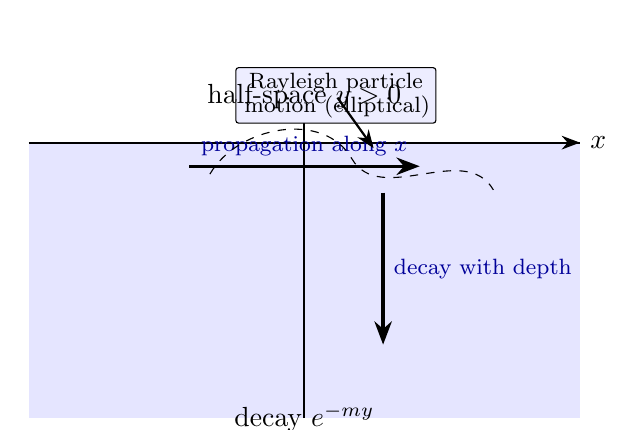
\begin{tikzpicture}[x=1.0cm,y=1.0cm,>=Stealth]
  \tikzset{
    node/.style={draw,rounded corners=1pt,fill=blue!7,align=center,font=\footnotesize,inner sep=2pt,text width=2.4cm},
    arr/.style={->,thick,shorten >=1pt,shorten <=1pt},
    lbl/.style={font=\footnotesize,text=blue!60!black},
    medium/.style={fill=blue!10},
  }
  % Half-space region
  \fill[medium] (-3.5,-3.5) -- (3.5,-3.5) -- (3.5,0) -- (-3.5,0) -- cycle;
  % Surface line
  \draw[thick] (-3.5,0) -- (3.5,0);
  % Axes
  \draw[->,thick] (-3.5,0) -- (3.5,0) node[right] {$x$};
  \draw[->,thick] (0,-3.5) -- (0,0.5) node[above] {$y$};
  % Propagation along x
  \draw[arr,very thick] (-1.5,-0.3) -- (1.5,-0.3) node[pos=0.5,above,lbl] {propagation along $x$};
  % Decay with depth
  \draw[arr,very thick] (1.0,-0.6) -- (1.0,-2.6) node[pos=0.5,right,lbl] {decay with depth};
  % Elliptical particle motion at surface
  \draw[dashed] (-1.2,-0.4) to[out=60,in=120] (0.6,-0.2) to[out=-60,in=120] (2.4,-0.6);
  \node[node] at (0.4,0.6) {Rayleigh particle\\[-1pt] motion (elliptical)};
  \draw[arr] (0.4,0.6) -- (0.9,-0.1);
  % Region labels
  \node[above] at (0,0.3) {half-space $y>0$};
  \node[below] at (0,-3.2) {decay $e^{-m y}$};
\end{tikzpicture}

\caption{Geometry after \citep{Rayleigh1885}: thermoelastic Rayleigh wave on a half-space -- surface-trapped particle motion decaying exponentially with depth, coupled dilatational--thermal and shear potentials.}\label{fig:rayleigh-geo}
\end{figure}

\subsection{Results}
\Cref{fig:rayleigh} shows the speed change and damping of the thermoelastic Rayleigh wave for $\varepsilon=0.05$, $\nu=0.3$. The speed increases by about $2\times10^{-3}$ at low wavenumber relative to the purely elastic Rayleigh speed (the adiabatic limit) and tends to the elastic value at large $k$ (the isothermal limit), in the same way as the bulk wave (\Cref{fig:disp}a), but the effect is about an order of magnitude smaller than for the compressional wave because only part of the surface motion is dilatational. The damping peaks at $k\,c_1/\omega_*\approx0.4$ with a quality-factor reciprocal of about $2\times10^{-3}$. The thermal boundary condition matters at low wavenumber: an isothermal surface shifts the damping peak to smaller $k$ and lowers the speed change, since the surface temperature fluctuation is suppressed. The Lord--Shulman law ($\tau_q=0.25/\omega_*$, insulated surface) changes the results little at low wavenumber but increasingly at large $k$: relative to the classical insulated surface the damping differs by less than $1\,\%$ for $k\,c_1/\omega_*\le0.1$, by $5\,\%$ at the damping peak, by $10\,\%$ at $k\,c_1/\omega_*=1$ and saturates at about $12\,\%$ for $k\,c_1/\omega_*\ge10$; the speed offset is $-1.2\times10^{-4}$ in relative terms at large $k$. This is the pattern expected from the bulk wave: the heat law matters once the product of the frequency and the lag is of order one.

\begin{figure}[t]\centering
\includegraphics[width=\textwidth]{figs/fig_rayleigh.pdf}
\caption{Thermoelastic Rayleigh wave in a half-space ($\nu=0.3$, $\varepsilon=0.05$). (a) Speed relative to the purely elastic Rayleigh speed. (b) Temporal damping $Q^{-1}=2|\Imag\omega|/\Real\omega$ at real wavenumber $k$ in units of $\omega_*/c_1$. Curves: classical theory with insulated and with isothermal surface, and Lord--Shulman with $\tau_q=0.25/\omega_*$ and insulated surface.}\label{fig:rayleigh}
\end{figure}

\subsection{Anisotropic, piezoelectric and nonlocal surface waves}
For anisotropic media the Stroh formalism \citep{Stroh1958,Stroh1962} gives the displacement--traction state vector as a first-order system in $y$, and the secular equation becomes the vanishing of a $3\times3$ (or larger, when piezoelectric and thermal fields are added) determinant built from the eigenvectors with decaying exponents; this is the route taken for piezothermoelastic layers and half-spaces \citep{Biswas2020}. For piezoelectric materials, new surface-wave types arise: the Bleustein--Gulyaev shear-horizontal wave exists for transversely isotropic piezoelectric substrates even though a pure SH wave cannot exist at an ordinary elastic free surface; Rayleigh waves in nonlocal piezoelastic half-spaces and piezo-thermoelectric semiconductors have been treated with Eringen-type nonlocality and with fractional or Klein--Gordon-type extensions \citep{Tung2019,Gupta2024,Aldandani2026,Lazar2022}. Energy aspects of surface thermoelastic waves are discussed in \citep{IvanovSavova1991}. In each of these extensions the structure of the problem is identical to the determinant above, with additional exponents and boundary conditions; the physical effects are the shift of the Rayleigh root by electromechanical stiffening (by $K^2$, see Section~\ref{sec:multi}), by nonlocal dispersion (Section~\ref{sec:size}), and by thermal damping as shown here.

\subsection{Practical remarks on secular equations}
Three technical points recur. (i) The decaying branch of each square root must be chosen with $\Real m>0$, and in the complex plane this introduces branch cuts across which the determinant is not analytic; root finding that ignores this can jump to spurious roots. (ii) The determinant has trivial zeros ($s=0$ for instance) that must be excluded when tracking roots; we found that a naive secant search from a poor initial guess converged to such a trivial root. (iii) Continuation in $k$ from a reliable starting point (here the isothermal Rayleigh root) is more robust than independent root finding at each $k$.

\begin{summarybox}[Summary]
The thermoelastic Rayleigh problem is a $3\times3$ determinant \mathcal D(s,k) from two coupled dilatational--thermal modes and one shear mode, with insulated or isothermal surface. Speed shifts from adiabatic (low $k$) to elastic/isothermal (high $k$); damping peaks near $k c_1/\omega_*\approx0.4$. The thermal boundary condition shifts the peak; LS changes results by $\sim$10--12\% at large $k$.
\end{summarybox}

\section{Thermoelastic Lamb waves in a plate}\label{sec:lamb}

Surface waves on a half-space (\cref{sec:surface}) have a counterpart in plates, where the two free faces couple the dilatational, shear and thermal fields. The plate problem is where the flexural thermoelastic damping of \cref{sec:flexted} is recovered from the full field equations, which gives a stringent test of the formulation.

\subsection{Formulation}
Consider a plate $-h<y<h$ in plane strain, with waves $\exp[i(kx-\omega t)]$ along $x$ and real $k$. The fields are the two dilatational--thermal modes $j=1,2$, which are the two roots $\kappa_j$ of the coupled quadratic of \cref{sec:classical} with transverse wavenumbers $m_j=\sqrt{\kappa_j+k^2}$, and the shear mode with $m_s=\sqrt{s^2/c_2^2+k^2}$ with $s=-i\omega$. Each mode appears as $e^{\pm m y}$, so there are six amplitudes. The boundary conditions on $y=\pm h$ are $\sigma_{yy}=\sigma_{xy}=0$ and either an insulated ($\theta_{,y}=0$) or an isothermal ($\theta=0$) face, which gives a $6\times6$ determinant $D(s;k,h)$ whose roots are the plate modes. For a given real $k$ the roots $s$ are complex, and $Q^{-1}=2|\operatorname{Im}\omega|/\operatorname{Re}\omega$ measures the temporal damping. The heat-flux model enters only through $G(s)$ in the quadratic, so lagging and fractional laws are handled by substitution. The implementation is in \path{scripts/lamb_te.py}.

\subsection{Validation}
Two checks were made.
\begin{enumerate}
\item \emph{Elastic limit.} With $\varepsilon=10^{-8}$ and $kh=0.3$ the antisymmetric root is $\omega=0.04426280008$ (units $c_1=1$, $h=1$), against $0.04426280008$ from the Rayleigh--Lamb equation $\tan(qh)\,4k^2pq+(q^2-k^2)^2\tan(ph)=0$ solved separately; they agree to about $10^{-10}$.
\item \emph{Thin-plate thermoelastic damping.} For $\varepsilon=0.05$, $\nu=0.3$ and a plate with $h=20\,c_1/\omega_*$ the loss of the lowest antisymmetric mode was computed over $10^{-3}\lesssim kh\lesssim1.3$. For $\omega\ll\omega_Z=\pi^2\chi/(2h)^2$ the loss follows \cref{eq:LR} with the plane-strain value $\Delta=E\alpha_T^2T_0(1+\nu)/[(1-\nu)c_v]$, with ratio $1.000$ for $kh\lesssim0.015$, $0.998$ at $kh=0.036$, and $0.989$ at $kh=0.088$.
\end{enumerate}
The factor $(1+\nu)/(1-\nu)$ rather than $1$ is what plane strain requires (stiffness $E/(1-\nu^2)$ and expansion $(1+\nu)\alpha_T$), and the numerics confirm it. A beam formula quoted with the uniaxial $\Delta$ would underestimate the plane-strain damping by a factor $1.86$ at $\nu=0.3$.

\subsection{Beyond the thin-plate limit}
\Cref{fig:lambte} shows the loss and its ratio to \cref{eq:LR}. The ratio falls to $0.94$ at $kh=0.22$, to $0.77$ at $kh=0.53$ (where $\omega=1.01\,\omega_Z$) and to $0.71$ at $kh=1.3$. The peak loss is $Q^{-1}=7.6\times10^{-3}$ at $\omega/\omega_Z=1.01$, against $9.9\times10^{-3}$ for the thin-plate formula. Thus the thin-plate formula overestimates the loss by about $30\%$ at the peak once the wavelength is only a few thicknesses, presumably because shear and rotary-inertia effects, absent from the Euler--Bernoulli kinematics behind \cref{eq:LR}, become important; this computation does not isolate that cause. Resonator designs with $kh\gtrsim0.3$ therefore need the full determinant or a Mindlin-type thermoelastic model.

\begin{figure}[t]
\centering
\includegraphics[width=\linewidth]{figs/fig_lamb_te.pdf}
\caption{Lowest antisymmetric (flexural) mode of a thermoelastic plate, plane strain, $\varepsilon=0.05$, $\nu=0.3$, $h=20\,c_1/\omega_*$, insulated faces. (a) Loss from the $6\times6$ determinant and from \cref{eq:LR} with the plane-strain $\Delta$. (b) Ratio of the two against $kh$.}
\label{fig:lambte}
\end{figure}

\subsection{Role of the heat-flux law}
In \cref{eq:LR} heat flows across the thickness, so the relevant dimensionless number is the product of the lag with the transverse relaxation rate $\omega_Z=\pi^2\chi/(2h)^2$. For thicknesses of several tens of nanometres in metals, $\tau_q\omega_Z\ll1$ and the parabolic result is adequate (\cref{sec:flexted}); for sub-ten-nanometre films, or when the phonon mean free path is comparable to the thickness, a kinetic or Guyer--Krumhansl treatment (\cref{sec:kinetic}) is the more appropriate refinement. The determinant above does not by itself settle which regime applies; it only provides the correct reference result for each choice of $G(s)$.

\section{Resonant modes of a clamped bar}\label{sec:bar}

The loss measured in a resonator is a temporal quantity: a standing mode with real wavenumber $k_n=n\pi/L$ decays in time with a complex frequency $\omega_n$. Here the plane-wave polynomial of \cref{eq:unified} is used with real $k$ and complex $s=-i\omega$.

\subsection{Setting}
Take a bar of length $L$ with both ends clamped ($u=0$) and insulated ($\theta_{,x}=0$). Each eigenfunction has the form $u\propto\sin k_nx$, $\theta\propto\cos k_nx$ with $k_n=n\pi/L$, so the boundary conditions are satisfied exactly by each coupled mode and the modal frequencies are the roots of the polynomial of \cref{eq:unified} in $s$ at $K=k_n^2$. For Lord--Shulman heat flux the polynomial is quartic in $s$, for the classical law cubic. The mode tracked is the elastic-like root, followed by continuity in $k$ from the adiabatic starting value $c_1\sqrt{1+\varepsilon}\,k$. In units $c_1=\omega_*=1$ and with $\varepsilon=0.1$ the results of the script \path{scripts/fig_bar_modes.py} are as follows.

\subsection{Results}
\begin{itemize}
\item At small $k$ all models give the same loss (numerically $8.7\times10^{-4}$ at $k=0.01$), about $13\%$ below the first-order Debye value $\varepsilon k/(1+k^2)$ because of the $O(\varepsilon)$ difference between temporal and spatial loss measures.
\item The classical law gives a Debye-type peak $Q^{-1}=0.0488$ at $k\,c_1/\omega_*=1.07$, and the modal speed falls from the adiabatic value $1.049\,c_1$ to $c_1$ at large $k$.
\item For Lord--Shulman with $\tau\omega_*=0.25$ the peak rises to $0.0676$ at $k=1.39$, and the high-$k$ modal speed settles at $0.984\,c_1$.
\item For $\tau\omega_*=1$, where the thermal front speed equals $c_1$, the peak is $0.146$ at $k=1.84$, three times the classical value, and the high-$k$ modal speed is $1.17\,c_1$. This is the degenerate case of equal front speeds, where the two fronts split by coupling to $c^2=c_1^2[1+\varepsilon/2\pm\sqrt{\varepsilon+\varepsilon^2/4}]$, giving $1.17\,c_1$ for the upper root.
\end{itemize}
The curves are shown in \cref{fig:barmodes}. Near $\tau\omega_*\approx1$ the thermal and elastic branches hybridise, so the label ``elastic-like'' ceases to be sharp and results must be read together with the branch-tracking procedure.

\begin{figure}[t]
\centering
\includegraphics[width=\linewidth]{figs/fig_bar_modes.pdf}
\caption{Loss $Q^{-1}=2|\operatorname{Im}\omega|/|\operatorname{Re}\omega|$ and modal speed of the elastic-like mode of a clamped insulated bar ($\varepsilon=0.1$) against $k=n\pi/L$ for classical and Lord--Shulman heat flux.}
\label{fig:barmodes}
\end{figure}

\subsection{Consequence for resonator design}
A bar of fixed length and a sequence of overtones traverse the curve of \cref{fig:barmodes} from left to right. The classical model predicts the worst loss when $k_nc_1\approx\omega_*$, and the lag raises it only if $\tau\omega_*$ is of order one, where the lag law is also least trustworthy. For all materials of \cref{tab:materials} $\omega_*$ exceeds $10^{11}$\,rad/s, so the position of the peak lies at wavelengths of order $c_1/\omega_*\sim10$\,nm, and bar resonators of micron size operate on the left, linear-in-$k$ flank where the models coincide.

\begin{summarybox}[Summary]
A clamped bar's overtones trace the thermoelastic damping curve from left to right. Classical theory predicts worst loss at $k_nc_1\approx\omega_*$; lagged models raise it only if $\tau\omega_*\sim1$, where the lag law is least trustworthy. For all materials of Table~\ref{tab:materials}, $\omega_*>10^{11}$\,rad/s, so micron-scale bar resonators operate on the linear-in-$k$ flank where all models agree.
\end{summarybox}

\section{Interfaces, reflection and energy partition}\label{sec:interfaces}
Reflection and transmission at interfaces is the most heavily studied wave problem in generalized thermoelasticity and multiphysics media; Table~\ref{tab:streams} lists many of the works. Most of them report \emph{energy ratios} and use the requirement that the ratios sum to unity as a validation. This section builds the problem from the elastic baseline, then adds thermal coupling and shows when and why the unit-sum check is satisfied or violated, since this is a point on which the literature is not uniform.

\subsection{Welded elastic interface at normal incidence}
Two elastic half-spaces with impedances $Z_j=\rho_jc_{1j}$ are perfectly bonded at $x=0$. For a wave incident from medium~1, continuity of displacement and of traction gives the displacement amplitude coefficients
\begin{equation}
r=\frac{Z_1-Z_2}{Z_1+Z_2},\qquad t=\frac{2Z_1}{Z_1+Z_2},\label{eq:rt}
\end{equation}
and the time-averaged energy fractions $\mathcal R=r^2$, $\mathcal T=4Z_1Z_2/(Z_1+Z_2)^2$ satisfy $\mathcal R+\mathcal T=1$ (\Cref{fig:interface}). The displacement transmission coefficient $t$ can reach two for a soft second medium without violating conservation, since only the energy fractions are bounded.
\begin{figure}[t]\centering
\includegraphics[width=\textwidth]{figs/fig_interface.pdf}
\caption{Normal incidence on a welded elastic interface. (a) Displacement reflection and transmission coefficients. (b) Energy fractions; $\mathcal R+\mathcal T=1$ for every impedance ratio.}\label{fig:interface}
\end{figure}

\subsection{Oblique incidence on an elastic interface}
For oblique incidence of a P wave, Snell's law conserves the horizontal slowness $p=\sin\theta_1/c_{1,P}=\sin\phi_1/c_{1,S}=\sin\theta_2/c_{2,P}=\sin\phi_2/c_{2,S}$ and four waves are generated (reflected P and SV, transmitted P and SV). Continuity of $u_x,u_z,\sigma_{zz},\sigma_{xz}$ gives four linear equations for the amplitudes (the Zoeppritz system). We solved it for a pair of media ($\rho_1,c_P,c_S=2.5,5.0,2.8$ and $\rho_2,c_P,c_S=3.0,8.0,4.5$ in arbitrary consistent units), with energy flux per wave $P_z=-\tfrac12\Real(\sigma_{zj}\overline{\dot u_j})$. The sum of the four energy fractions equals one to rounding error ($|\text{sum}-1|<2\times10^{-15}$ over $0.5^\circ$--$89.5^\circ$), and at normal incidence the P--P reflection fraction ($0.099268$) equals the impedance formula ($0.099268$). \Cref{fig:ienergy}(a) shows the characteristic features: a critical angle ($38.7^\circ$ here), beyond which the transmitted P wave is evanescent and carries no energy; a rise of the reflected P fraction to total reflection of P energy in the P--P channel only at grazing incidence, with mode conversion in between.

\subsection{Thermoelastic interfaces}
When both media are thermoelastic, two further wave types appear in each medium and the interface conditions include thermal continuity. For perfect thermal contact, $\theta$ and the normal flux $q_n$ are continuous together with displacement and traction. In normal incidence there are four amplitudes (reflected elastic and thermal waves, transmitted elastic and thermal waves) and four equations. We implemented this for two media with different densities, wave speeds, heat capacities, conductivities, coupling constants and lag times, with Lord--Shulman conduction; incident wave of elastic type. The amplitude ratios and the flux of each wave follow from \eqref{eq:P}. The tests we performed are: (i) as $\varepsilon\to0$ (here $\beta=10^{-6}$) the reflected elastic energy fraction ($0.169550173$) equals the impedance formula $(Z_1-Z_2)^2/(Z_1+Z_2)^2$ to twelve digits; (ii) the \emph{net} flux, computed from the total fields on either side of the interface, is continuous to $10^{-15}$ for all frequencies tested.

\paragraph{When does ``energy fractions sum to one'' hold?} The exact statement is item (ii): the net flux of \eqref{eq:P} into the interface equals the net flux out of it, because the continuity conditions imply continuity of $\sigma\dot u$ and of $\theta q$. This is not the same as saying that the \emph{sum of the fluxes carried by each wave separately} equals the incident flux. For homogeneous waves in lossless media the two statements coincide, because the cross terms between distinct modes vanish in the time average (this is what the elastic checks above confirm numerically). In a dissipative medium, the modes have complex wavenumbers and the cross terms between, for example, the elastic-type and the thermal-type wave at the interface do not vanish, so
\begin{equation}
\sum_n\mathcal F_n\ne1\quad\text{in general, while}\quad \mathcal F_{\rm net}\equiv1.
\end{equation}
\Cref{fig:ienergy}(b,c) shows an example: the sum of the four mode fractions is within $1.5\,\%$ of unity for $\omega\lesssim2\omega_*$ but reaches 1.34 near $\omega\approx8\omega_*$ and individual fractions can exceed one (the transmitted elastic fraction reaches 1.1). This is not a violation of energy conservation: the cross terms account for the difference. The consequence for published results is practical. An energy-ratio sum that deviates from unity can be caused by (a) a wrong coupling coefficient or boundary condition, (b) a flux definition inconsistent with the model, or (c) genuine interference of modes in a dissipative medium; the first two are errors, the third is not, and a correct check must use the net flux, or include the interference terms, rather than the sum of mode fluxes. Studies that report energy ratios at thermoelastic and piezothermoelastic interfaces \citep{Barak2023,Barak2023IJP,Barak2023JTS,Barak2023MMMS,Gupta2023Energy,Kumar2023PhysScr,Kumar2019,Kumar2022,Kumar2024,Kumar2024a} should be read with this point in mind: when the media are lossy, a unit sum of mode ratios is not a necessary condition and a failure of the sum to equal one is not by itself evidence of error.

\begin{figure}[t]\centering
\includegraphics[width=\textwidth]{figs/fig_interface_energy.pdf}
\caption{Energy partition at welded interfaces. (a) Oblique P incidence on an elastic--elastic interface: reflected and transmitted P and SV energy fractions; their sum is unity at every angle. (b) Normal incidence on a thermoelastic--thermoelastic interface with Lord--Shulman conduction ($\varepsilon_1=0.1$, $\varepsilon_2=0.3$, $\tau_{q1}=0.25/\omega_*$, $\tau_{q2}=0.15/\omega_*$): energy fractions of the four generated waves against frequency. (c) The sum of mode fractions deviates from unity at high frequency because of interference terms, while the net flux of \eqref{eq:P} is continuous across the interface (dashed).}\label{fig:ienergy}
\end{figure}

\subsection{Imperfect interfaces}
Real interfaces are rarely perfect. The common idealisation replaces continuity by spring conditions: the traction is continuous and proportional to the jump in displacement, $\sigma=K_n[u]$ (normal) and $K_t[u_t]$ (tangential); thermal imperfections add a thermal contact resistance, $[\theta]=R_\theta q$ (the Kapitza-type jump), and for micropolar or piezoelectric media analogous electric and rotational conditions. In the limit $K\to\infty$ one recovers the welded interface and for $K\to0$ a free surface. With thermal resistance the net flux of \eqref{eq:P} is no longer continuous: the jump $[\theta]q/T_0=R_\theta q^2/T_0$ is the entropy production at the interface, and the energy balance must include it. Imperfect-interface wave problems have been treated for micropolar solids \citep{Fu2013}, piezoelectric composites \citep{Kumawat2023,Gupta2025}, and a fluid--double-porous thermoelastic interface \citep{Kumar2025}.

\subsection{Fluid--solid and multiphysics interfaces}
When one medium is an ideal fluid the shear conditions change (no shear traction, tangential displacement discontinuous), and the energy ratios have been computed for fluid--piezothermoelastic and fluid--double-porous interfaces \citep{Gupta2023IJNMF,Kumar2019,Kumar2025}. In piezoelectric media electric boundary conditions (continuity of potential and of normal electric displacement, or an electrode condition) add two equations per interface; the reflection and refraction at elastic--magneto-thermoelastic diffusion solids with voids \citep{KumarKansal2017}, micropolar piezothermoelastic half-spaces \citep{Kumar2018}, functionally graded piezoelectric microstructures \citep{Liu2020} and flexoelectric or flexomagnetic microstructures \citep{Singh2020c,Jiao2024} extend the same procedure. All of these share the structure of Sections~\ref{sec:surface} and the present one: a linear system for amplitudes whose entries are fixed by the dispersion roots of each medium, and an energy flux that must be defined consistently with the model.

\subsection{A checklist for interface calculations}
The following checks, which cost little, catch most errors in interface calculations:
\begin{enumerate}
\item Reduce the coupling to zero and compare with the elastic impedance formulas (normal incidence) or the Zoeppritz equations.
\item Verify the Snell invariants (horizontal slowness) for all generated waves, including evanescent ones.
\item Verify continuity of the net flux \eqref{eq:P} (not of the sum of mode fluxes) across a perfect interface; for imperfect interfaces include the interface dissipation.
\item Test the boundary conditions independently: substitute the computed amplitudes back into each boundary equation.
\item For lagged and memory models, state the flux definition used for the energy ratio and whether interference terms are included.
\end{enumerate}

\section{Size effects: nonlocal and gradient models}\label{sec:size}
\subsection{Why local elasticity fails at small wavelengths}
Local elasticity predicts non-dispersive waves, $\omega=c\,k$, for all wavelengths. A crystal is a lattice, and its acoustic branch bends over and reaches zero group velocity at the zone boundary. For a monatomic chain with nearest-neighbour spring constant $\kappa_s$, mass $m$ and spacing $a$, the exact relation is $\omega=2\sqrt{\kappa_s/m}\,|\sin(ka/2)|=c_0k\,\mathrm{sinc}(ka/2)$ with $c_0=a\sqrt{\kappa_s/m}$ \citep{BornKarman1912}, which at small $k$ gives $\omega\simeq c_0k\,[1-(ka)^2/24]$. Nonlocal and gradient models add one length scale to capture the leading deviation from local behaviour in a continuum framework. Maranganti and Sharma \citep{Maranganti2007} estimate the scales at which classical elasticity breaks down for various materials, and show that size effects can also generate electromechanical coupling in non-piezoelectric solids \citep{Maranganti2006}. Micropolar thermoelasticity without energy dissipation was formulated by Ciarletta \citep{Ciarletta1999} and Quintanilla \citep{Quintanilla2002}; strain gradient and higher-order nonlocal formulations appear in \citep{Gao2007,Lim2015,Ke2014}.

\subsection{Eringen's nonlocal elasticity}
In the integral model the stress at $\bx$ is a weighted average of the local stress over a neighbourhood,
$\sigma_{ij}(\bx)=\int\alpha(|\bx-\bx'|)\,C_{ijkl}\varepsilon_{kl}(\bx')\,\dd V'$, with a kernel $\alpha$ normalised to unity. For the exponential kernel in one dimension, $\alpha(|x|)=e^{-|x|/\ell}/(2\ell)$, the integral equation is equivalent to the differential equation
\begin{equation}
\bigl(1-\xi^2\partial_x^2\bigr)\sigma=c\,\varepsilon,\qquad \xi=\ell,\label{eq:eringen}
\end{equation}
(because $\alpha$ is the Green's function of $1-\ell^2\partial_x^2$), and in three dimensions with the Yukawa-type kernel $e^{-r/\ell}/(4\pi\ell^2r)$ the equation $(1-\xi^2\nabla^2)\sigma_{ij}=C_{ijkl}\varepsilon_{kl}$ \citep{Eringen1972,Eringen1983,Eringen2002}. Substituting in the momentum balance gives
\begin{equation}
\omega^2=\frac{c_0^2k^2}{1+\xi^2k^2},\qquad v_g=\frac{c_0}{(1+\xi^2k^2)^{3/2}},\label{eq:erin}
\end{equation}
where $\xi=e_0a$ in Eringen's notation ($e_0$ a dimensionless material constant and $a$ an internal characteristic length). Equation~\eqref{eq:erin} is the rational analogue of the lattice relation: $\omega$ is bounded by $c_0/\xi$ and the group velocity decays to zero at large $k$.

\paragraph{Calibration against the lattice.} Matching \eqref{eq:erin} to the chain at the zone boundary $k=\pi/a$, where $\omega=2c_0/a$, requires $(\xi/a)^2=\tfrac14-1/\pi^2$, i.e.\ $\xi/a=0.3856$; this reproduces the value $e_0\approx0.39$ quoted by Eringen \citep{Eringen1983} and is the origin of the often-used choice. Matching instead the long-wavelength curvature requires $\xi^2=a^2/12$ ($\xi=0.289a$). The two calibrations differ by about one third in $\xi$ and thus by a factor of about $1.8$ in $\xi^2$, so any quantitative prediction that depends on $\xi$ depends on the calibration target (\Cref{fig:lattice}). The group velocity of the Eringen model at the zone boundary is $0.26c_0$, whereas the chain has $v_g=0$ there.

\subsection{Strain-gradient elasticity}
Aifantis-type gradient elasticity adds the gradient of the strain \citep{Aifantis1992,Aifantis2003},
\begin{equation}
\sigma=c\,(\varepsilon-\ell^2\varepsilon_{,xx}),\qquad \omega^2=c_0^2k^2(1+\ell^2k^2),\qquad v_g=c_0\frac{1+2\ell^2k^2}{\sqrt{1+\ell^2k^2}}.\label{eq:grad}
\end{equation}
Both phase and group velocities \emph{increase} with $k$ for $\ell^2>0$, the opposite of lattice dispersion. To reproduce the lattice curvature one needs $\ell^2=-a^2/12<0$, which gives $\omega^2=c_0^2k^2(1-a^2k^2/12)$ and an instability ($\omega^2<0$) beyond $k=\sqrt{12}/a$ --- outside the Brillouin zone, but a warning that the pure gradient model with the lattice sign is not well posed at high wavenumber. The dispersive-stabilised versions, with a gradient of inertia as well as of strain \citep{Askes2006,Askes2011}, interpolate between \eqref{eq:erin} and \eqref{eq:grad}: with strain-gradient length $\ell_s$ and inertia-gradient length $\ell_d$, $\omega^2=c_0^2k^2(1+\ell_s^2k^2)/(1+\ell_d^2k^2)$, which remains stable and reproduces the lattice shape for $\ell_d>\ell_s$ (the Eringen form is the case $\ell_s=0$).

\begin{figure}[t]\centering
\includegraphics[width=\textwidth]{figs/fig_lattice.pdf}
\caption{Nonlocal and gradient dispersion compared with the exact monatomic chain. (a) Dispersion: Eringen with two calibrations (zone-boundary and long-wavelength), gradient with positive and negative length-squared, and the local model. (b) Group velocity of the chain and of the Eringen model with the zone-boundary calibration.}\label{fig:lattice}
\end{figure}
\begin{figure}[t]\centering
\includegraphics[width=\textwidth]{figs/fig_nonlocal.pdf}
\caption{Generic size-effect dispersion for $\xi=\ell=0.5$ in units of the characteristic length. (a) Frequency against wavenumber: the Eringen model saturates at $c_0/\xi$, the gradient model rises faster than linearly. (b,c) Phase and group speeds.}\label{fig:nonlocal}
\end{figure}

\subsection{Other enrichments}
Couple-stress theory \citep{MindlinTiersten1962}, micropolar theory \citep{Eringen1966a,Eringen1999}, flexoelectricity and surface elasticity add length scales through different mechanisms. The Klein--Gordon-type nonlocal elasticity \citep{Lazar2022} (a Helmholtz-type operator acting on the displacement rather than the stress) has been used with piezo-thermoelastic media \citep{Das2026}. Nonlocal variational principles are discussed in \citep{Polizzotto2001}. The physical ingredients differ, but at the level of plane-wave dispersion most enrichments reduce to a rational function of $k^2$ multiplying the local stiffness or the inertia, and the choice among them is largely a matter of which feature of the underlying lattice or microstructure one wishes to represent.

\subsection{Nonlocal thermoelasticity}
Eringen \citep{Eringen1974} extended nonlocality to thermoelasticity. Two forms of the constitutive relation are in use in recent papers:
\begin{align}
\text{(A)}\quad & (1-\xi^2\partial_x^2)\,\sigma=c\,\varepsilon-\beta\theta, \\
\text{(B)}\quad & (1-\xi^2\partial_x^2)\,(\sigma+\beta\theta)=c\,\varepsilon,
\end{align}
that is, whether the thermal stress is smoothed with the elastic stress (B) or not (A). The two forms give different dispersion polynomials: with $K=k^2$, (A) is $\bigl[\rho(c_1^2+\xi^2s^2)K+\rho s^2\bigr](s\rho c+GK)+\beta^2T_0sK=0$, and (B) adds the factor $(1+\xi^2K)$ to the last term. Both reduce to the local relation \eqref{eq:disp} as $\xi\to0$ and to the nonlocal elastic relation \eqref{eq:erin} as $\varepsilon\to0$; we confirmed both limits numerically. \Cref{fig:nonlocal-te} compares the elastic-type branch. In the classical theory with $\varepsilon=0.1$ and $\xi=0.3c_1/\omega_*$ (elastic cut-off at $\omega=3.3\omega_*$), the main effect on the phase speed is the nonlocal dispersion itself: the speed falls steadily with frequency, to about $0.3c_1$ at $95\,\%$ of the cut-off, and the two forms give almost the same speed. The damping differs: form~(A) stays close to the local curve (its maximum is about $15\,\%$ larger and slightly shifted) whereas form~(B), whose thermal coupling is multiplied by $1+\xi^2K$ and thus grows with wavenumber, shows a damping that increases steeply on approaching the cut-off, reaching $Q^{-1}\approx0.3$. The difference arises entirely from the high-wavenumber coupling. A paper that reports nonlocal thermoelastic damping or dispersion should therefore state which form is used; the literature on nonlocal thermoelastic waves \citep{Tiwari2021,Sarkar2019,Lata2020,Bachher2019,Li2018,Kalkal2020,Kumar2023} uses various forms.
\begin{figure}[t]\centering
\includegraphics[width=\textwidth]{figs/fig_nonlocal_te.pdf}
\caption{Elastic-type branch of the nonlocal classical thermoelastic problem ($\varepsilon=0.1$, $\xi=0.3c_1/\omega_*$, frequency up to $95\%$ of the elastic cut-off $c_1/\xi$): phase speed (a) and damping (b) for the local model and the two nonlocal forms.}\label{fig:nonlocal-te}
\end{figure}

\subsection{Nonlocality in the heat flux}
The Guyer--Krumhansl equation \citep{GuyerKrumhansl1966,GuyerKrumhansl1966II} adds spatial derivatives of the flux,
\begin{equation}
q_i+\tau_R\dot q_i=-k\theta_{,i}+\ell_{GK}^2\bigl(\nabla^2q_i+2\,q_{j,ji}\bigr),
\end{equation}
and describes heat in the hydrodynamic phonon regime, where momentum-conserving collisions dominate. In one dimension the extra term is $3\ell_{GK}^2q_{,xx}$ and $G(s,k)=k/(1+\tau_Rs+3\ell_{GK}^2k^2)$ depends on the wavenumber, so the dispersion polynomial is no longer quadratic in $K$ but retains its structure. For low-temperature crystals, ballistic and size-dependent conduction in nanostructures are modelled with this and related equations; the combination with elastic nonlocality remains little explored (Section~\ref{sec:open}).

\subsection{Caveats}
The differential nonlocal model produces well-known inconsistencies for bounded bodies (for example in some bending problems with particular boundary conditions) that do not appear in the infinite-medium plane-wave analysis above. The length scales are phenomenological; whether the lattice, the zone-boundary or some experimental dispersion is the calibration target has a leading effect on the quantitative predictions.

\section{Coupling to further fields}\label{sec:multi}
Thermoelastic waves are one member of a larger class: whenever a further field is energetically coupled to deformation and temperature, the dispersion relation acquires additional branches or renormalised constants, and the heat-flux law acts as a module that can be exchanged without altering the coupling structure. This section treats the piezoelectric coupling in detail, because it admits an exact reduction, and then surveys the principal other couplings at the level of structure.

\subsection{Piezoelectric stiffening}
Consider a one-dimensional piezoelectric bar in the quasi-electrostatic approximation, with $E=-\varphi_{,x}$ and the magnetic field neglected \citep{Yang2018,MindlinTiersten1962}. The constitutive relations are
\begin{equation}
\sigma=c\,u_{,x}-e\,E,\qquad D=\varepsilon_e E+e\,u_{,x},
\end{equation}
with elastic constant $c$ at constant field, piezoelectric constant $e$ and permittivity $\varepsilon_e$ at constant strain. Gauss's law $D_{,x}=0$ (no free charge) gives $E=-(e/\varepsilon_e)u_{,x}$ up to a uniform field, so
\begin{equation}
\sigma=\Bigl(c+\frac{e^2}{\varepsilon_e}\Bigr)u_{,x},\qquad v=\sqrt{\frac{c+e^2/\varepsilon_e}{\rho}}=v_0\sqrt{1+K^2},\quad K^2=\frac{e^2}{\varepsilon_e c}.
\label{eq:piezo}
\end{equation}
The electromechanical coupling constant $K^2$ ranges from a fraction of a percent in weakly piezoelectric crystals to several tens of percent in strongly piezoelectric ceramics, so the stiffening, shown in \Cref{fig:piezo}, is large enough to matter in resonator design.
\begin{figure}[t]\centering
\includegraphics[width=0.5\textwidth]{figs/fig_piezo.pdf}
\caption{Piezoelectric stiffening of the longitudinal wave speed, \eqref{eq:piezo}.}\label{fig:piezo}
\end{figure}

\subsection{Thermopiezoelectric waves: exact renormalisation}
With a pyroelectric coefficient $p$ the relations extend to
\begin{equation}
\sigma=cu_{,x}-eE-\beta\theta,\qquad D=eu_{,x}+\varepsilon_eE+p\theta,\qquad \rho\eta=\beta u_{,x}+pE+\frac{\rho c_E}{T_0}\theta,
\end{equation}
the last being the entropy (the pyroelectric and thermal-stress coefficients enter symmetrically, as required by the existence of a thermodynamic potential \citep{Mindlin1974Thermopiezo,Nowacki1978,Chandrasekharaiah1984}). Eliminating $E$ through $D_{,x}=0$ gives a purely thermoelastic system with the renormalised constants
\begin{equation}
\tilde c=c+\frac{e^2}{\varepsilon_e},\qquad
\tilde\beta=\beta-\frac{ep}{\varepsilon_e},\qquad
\rho\tilde c_v=\rho c_E-\frac{T_0p^2}{\varepsilon_e},\label{eq:renorm}
\end{equation}
and therefore all results of Sections~\ref{sec:classical}--\ref{sec:lags} hold with $c_1^2\to\tilde c/\rho$, $\beta\to\tilde\beta$, $c\to\tilde c_v$ in the definitions of $\varepsilon$ and $\omega_*$. We verified this reduction symbolically by computing the $3\times3$ determinant of the coupled system in $(u,\theta,\varphi)$ and comparing it with the renormalised thermoelastic polynomial: the ratio is a constant factor independent of all material parameters except the trivial scaling of the Gauss equation (script \path{check_thermopiezo.py}). Three observations follow. (i) The piezoelectric stiffening raises the isothermal speed by $\sqrt{1+K^2}$ and therefore changes $\omega_*$ and $\varepsilon$. (ii) The product $ep$ enters $\tilde\beta$ with a sign: depending on the orientation and sign conventions, the pyroelectric effect can \emph{reduce} or \emph{increase} the thermal stress, and the sign conventions for $e$ and $p$ vary across the literature, so a reported effect of the pyroelectric coefficient should be accompanied by a statement of conventions \citep{Yang2018}. (iii) The heat capacity under zero electric displacement ($D=0$) is smaller than under zero field, by $T_0p^2/\varepsilon_e$, the electric analogue of the difference between adiabatic and isothermal elasticity.

\paragraph{Limits of the quasi-electrostatic model.} The model has no electromagnetic branch and is valid when elastic wave speeds are small compared with the speed of light and the wavelength is much smaller than the electromagnetic wavelength at the same frequency, which holds for acoustic waves in all practical piezoelectric solids but excludes polaritons and fully dynamic electromagnetic coupling.

\paragraph{Extensions in the literature.} Piezothermoelastic waves with memory and fractional heat laws, semiconductor effects (photo-excited carriers and plasma waves), nonlocal piezoelasticity and surface effects, flexoelectric microstructure, and functionally graded or viscous variants have been treated in a large body of work \citep{Gupta2023,Gupta2024a,Gupta2026HeatMap,Das2026,Zang2014,Li2018,Liu2020,Singh2020c,Kumar2024,Kumar2024a,Abouelregal2023,Srivastava2026}. The structural point of \eqref{eq:renorm} applies to all of those that retain a one-dimensional or plane-wave setting: the additional coupling to the electric field in the absence of free charges is an exact renormalisation, and only when carriers (semiconductors) or higher electric moments (flexoelectricity) are added does a genuinely new branch appear.

Three-phase-lag thermoelastic heat conduction with higher-order time-fractional derivatives was proposed by \citep{Abouelregal2019}; generalized thermoelasticity based on higher-order memory-dependent derivative with time delay was developed by \citep{Abouelregal2021}. Memory-dependent and fractional order analysis of the initially stressed piezo-thermoelastic medium was presented by \citep{Barak2023a}; electro-thermoelasticity theory with memory-dependent derivative heat transfer was formulated by \citep{Ezzat2016a}. Photo-thermo-piezo-elastic waves in semiconductor medium subject to distinct two temperature models were studied by \citep{Gupta2023a}; quasi-P wave through orthotropic piezo-thermoelastic materials subject to higher order fractional and memory-dependent effects was analysed by \citep{Gupta2023b}. Theory of two-temperature thermoelasticity without energy dissipation was given by \citep{Youssef2011}; two-temperature thermoelasticity without energy dissipation of Green--Naghdi model was studied by \citep{Youssef2014}.

\subsection{Magneto-thermoelasticity}
For a perfectly conducting solid in a uniform magnetic field $\bm H_0$, the Lorentz force $\mu_0\bm J\times\bm H_0$ acts as an additional body force. For a longitudinal wave along $x$ with $\bm H_0$ perpendicular to the propagation direction and the displacement along the propagation direction, $h=-H_0u_{,x}$, $J=-h_{,x}$ and the force is $\mu_0H_0^2u_{,xx}$, so that $\rho\ddot u=(\lambda+2\mu+\mu_0H_0^2)u_{,xx}-\beta\theta_{,x}$. The magnetic field thus adds the Alfv\'en term to the stiffness, $c_1^2\to c_1^2+v_A^2$ with $v_A^2=\mu_0H_0^2/\rho$, and the dispersion polynomial \eqref{eq:disp} holds with that substitution. Finite electrical conductivity and displacement current add a magnetic diffusion branch and a further coupling that depends on the conductivity \citep{Ezzat2011,Ezzat2004,Ezzat2010,Bayones2021,Biswas2019,KumarKansal2017}; the fractional-order heat-conduction law in magneto-thermoelasticity of \citep{Ezzat2011} is a standard reference. Magneto-electro-thermo-elastic solutions for transversely isotropic media are given in \citep{Chen2004}; modified fractional-order piezoelectric thermoelasticity models appear in \citep{Guo2018,Mondal2020}.

\subsection{Thermoelastic diffusion and chemical coupling}
When a diffusing species is present, the concentration $C$ and chemical potential add a third field: the stress contains a term proportional to $C$, the energy balance a term proportional to $\dot C$ and the species balance a diffusive flux coupled to temperature. The dispersion polynomial becomes cubic in $K$ and a third, diffusive branch appears, with decay governed by the mass diffusivity. Higher-order and multi-lag diffusion models have been proposed \citep{Abouelregal2020a}, and reflection at interfaces with magneto-thermoelastic diffusion solids with voids has been computed \citep{KumarKansal2017}.

\subsection{Microstructure: micropolar, voids and porosity}
Micropolar elasticity \citep{Eringen1966a,Eringen1999,TauchertClausAriman1968} adds microrotation as an independent field. In the isotropic case the dilatational wave is accompanied by a longitudinal wave of modified speed, the transverse waves couple to microrotation waves, and the rotational waves have a cut-off frequency. Materials with voids \citep{Nunziato1979,Cowin1983,Iesan1986} add an independent volume-fraction field and one extra dilatational wave; thermal coupling is introduced in \citep{Iesan1986}; poro-thermoelasticity and double porosity add slow dilatational waves associated with pore fluid pressure \citep{Singh2020,Kumar2022,Kumar2025}. Fractional-order thermoelasticity with voids, micropolar fractional models and two-temperature versions have been studied \citep{Bachher2019,Sharma2022,Biswas2020a,Kalkal2020,Kumar2008,Kumar2018}. Each microstructural field adds branches that appear as new roots of the characteristic equation; whether they are physically observable depends on the microinertia and the coupling coefficients, which are usually assigned values with limited experimental support.

\subsection{Table of couplings}
\begin{figure}[t!]\centering\small
% fig8_multi.tex -- Multiphysics coupling geometry (s13_multiphysics)
\begin{tikzpicture}[x=1.0cm,y=1.0cm,>=Stealth]
  \tikzset{
    node/.style={draw,rounded corners=1pt,fill=blue!7,align=center,font=\footnotesize,inner sep=2pt,text width=2.4cm},
    arr/.style={->,thick,shorten >=1pt,shorten <=1pt},
    lbl/.style={font=\footnotesize,text=blue!60!black},
  }
  \node[node] at (-3.4, 0.8) (mech) {Mechanical\\[-1pt] $\\bu,\\varepsilon,\\sigma$};
  \node[node] at ( 1.4, 0.8) (therm) {Thermal\\[-1pt] $\\theta,q,T_0$\\[-1pt] heat law $G(s)$};
  \node[node] at (-3.4,-2.2) (elec) {Electric\\[-1pt] $E,D,\\varphi$\\[-1pt] piezo $e$, $\\varepsilon_e$};
  \node[node] at ( 1.4,-2.2) (mag) {Magnetic\\[-1pt] $\\bm H,\\bm J$\\[-1pt] Alfv\'en $v_A$};
  \node[node] at (-1.0,-4.2) (diff) {Diffusive\\[-1pt] concentration\\[-1pt] chemical potential};
  \draw[arr] (mech.east) -- (therm.west) node[pos=0.5,above,lbl] {$-\\beta\\nabla\\theta$};
  \draw[arr] (therm.west) -- (mech.east) node[pos=0.5,below,lbl] {dilatation heating};
  \draw[arr] (mech.south) -- (elec.north) node[pos=0.5,left,lbl] {$e\\nabla\\varphi$};
  \draw[arr] (therm.south) -- (mag.north) node[pos=0.5,right,lbl] {Lorentz force};
  \draw[arr] (elec.south) -- (diff.north) node[pos=0.5,left,lbl] {carriers};
\end{tikzpicture}

\caption{Geometry after \citep{Nowacki1978,Chandrasekharaiah1984}: multiphysics coupling -- each added field renormalises constants and/or adds branches; with no free charge the piezo-electric effect is an exact stiffening renormalisation.}\label{fig:multi-geo}
\end{figure}

\begin{table}[t]\centering\small
\caption{Added fields and their effect on the plane-wave problem (structure only; $\Delta n$ is the increase in the number of branches in one-dimensional dilatational motion).}\label{tab:couplings}
\begin{tabularx}{\textwidth}{@{}p{3.1cm}p{3.2cm}p{1.9cm}X@{}}\toprule
Added field & Principal effect on waves & $\Delta n$ & Remarks\\\midrule
Electric (quasi-static, no free charge) & stiffness $c\to c+e^2/\varepsilon_e$; $\beta$, $c_v$ renormalised & 0 & Exact reduction, Eq.~\eqref{eq:renorm}.\\
Electric with carriers (semiconductor) & plasma / diffusive branch & $+1$ & Photo-thermo-elastic and piezo-semiconductor models.\\
Magnetic (perfect conductor) & stiffness $c_1^2\to c_1^2+v_A^2$ & 0 & Finite conductivity adds a diffusion branch.\\
Concentration (diffusion) & third diffusive branch & $+1$ & Coupling to temperature through the chemical potential.\\
Voids / porosity & extra dilatational wave(s) & $+1$ (single) $+2$ (double) & Slow waves, strong damping.\\
Microrotation (micropolar) & rotational waves with cut-off & transverse & Longitudinal speed modified.\\
Two temperatures & wavenumber-dependent $\theta$ vs.\ $\varphi$ & 0 & Acts like a length scale.\\\bottomrule
\end{tabularx}
\end{table}

\begin{summarybox}[Summary]
Adding a field energetically coupled to deformation and temperature renormalises constants and/or adds branches. Piezoelectric stiffening with no free charge is an exact reduction ($c\to c+e^2/\varepsilon_e$, $\beta,c_v$ renormalised). Magnetic field adds the Alfv\'en term; diffusion adds a branch; voids and micropolarity add extra waves. All such couplings share the same dispersion-polynomial structure: solve the coupled system, then read speeds and damping from its roots.
\end{summarybox}

\section{Piezoelectric shear-horizontal surface waves}\label{sec:bg}

The thermopiezoelectric coupling of \cref{sec:multi} changes bulk stiffness, but piezoelectric media also support surface waves that have no elastic counterpart. The simplest is the Bleustein--Gulyaev (BG) wave, a shear-horizontal (SH) wave localised at the surface of a hexagonal (6mm) crystal. It is included here because it is the prototype of electromechanical surface localisation and because its closed form allows a clean statement of how the electrical boundary condition enters.

\subsection{Formulation}
Let the half-space $y>0$ be a 6mm crystal with the polar axis along $z$ and motion $u_z(x,y,t)$ polarised along $z$, with wave number $k$ along $x$. The relevant constants are the shear stiffness $c_{44}$, piezoelectric constant $e_{15}$ and permittivity $\varepsilon$, combined in $K^2=e_{15}^2/(c_{44}\varepsilon)$ and the stiffened modulus $\bar c=c_{44}(1+K^2)$ with bulk speed $\bar v=\sqrt{\bar c/\rho}$. In the quasi-static approximation the fields are $u=A\,e^{-\alpha y}$ and $\varphi=(e_{15}/\varepsilon)\,u+B\,e^{-ky}$, with $\alpha=k\sqrt{1-v^2/\bar v^2}$, and in the vacuum $y<0$ the potential is $\varphi=C\,e^{ky}$. The boundary conditions at $y=0$ are a free surface $\sigma_{yz}=c_{44}u_{,y}+e_{15}\varphi_{,y}=0$ together with either of the following:
\begin{itemize}
\item \emph{metallised surface}, $\varphi=0$;
\item \emph{free (unmetallised) surface}, continuity of $\varphi$ and of $D_y$ across the interface with vacuum permittivity $\varepsilon_0$.
\end{itemize}

\subsection{Results}
Eliminating the amplitudes gives the closed forms
\begin{equation}\label{eq:bg}
\frac{\alpha}{k}=\frac{K^2}{1+K^2}\ \ (\text{metallised}),\qquad
\frac{\alpha}{k}=\frac{\varepsilon_0}{\varepsilon+\varepsilon_0}\,\frac{K^2}{1+K^2}\ \ (\text{free}),
\end{equation}
so that the surface wave speed is $v=\bar v\sqrt{1-(\alpha_\ast/k)^2}$ with $\alpha_\ast/k$ from \cref{eq:bg}. These were checked against the numerical roots of the $3\times3$ secular determinant (script \path{scripts/check_bg.py}), which agree to the digits quoted. For $K^2=0.2$, $\bar v=1.0954\,v_t$ (with $v_t=\sqrt{c_{44}/\rho}$), the metallised speed is $1.0801\,v_t$, i.e.\ $1.4\%$ below $\bar v$, while for the free surface $v=1.0954$, $1.0953$ and $1.0916\,v_t$ for $\varepsilon_0/\varepsilon=0.01,\,0.1$ and $1$. For $K^2=0.5$ the metallised value is $1.1547\,v_t$ against $\bar v=1.2247\,v_t$.

Two consequences follow. First, the shift between free and metallised speeds, the usual electromechanical coupling measure of a surface wave, is of order $K^4$ and therefore small when $K^2$ is small. Second, the decay length $1/\alpha$ is very sensitive to the electrical condition: for $K^2=0.2$ it is about $1/k\cdot6$ (roughly one wavelength) when metallised, but about $600/k$ (roughly $100$ wavelengths) for a free surface with $\varepsilon_0/\varepsilon=0.01$. A plate of a few wavelengths thickness therefore does not support the free-surface BG wave as a surface wave in a strict sense.

\subsection{Thermal coupling}
For this SH polarisation with uniform fields in $z$ the shear strains $\epsilon_{xz},\epsilon_{yz}$ do not couple to the (diagonal) thermal-stress tensor of a hexagonal crystal, and the pyroelectric coupling acts along the polar axis $z$, which is perpendicular to the in-plane electric field. The BG wave is therefore not coupled to temperature in this geometry, and thermal effects enter only through the temperature dependence of $c_{44}$, $e_{15}$ and $\varepsilon$, which shifts the speed without introducing a loss. Coupled thermo-piezoelectric surface waves exist for other cuts and polarisations, where the sagittal-plane motion has a dilatational component, and for those the Rayleigh-type determinant of \cref{sec:surface} has to be extended by the electrical conditions.

\section{Solution methods and verification}\label{sec:methods}
\subsection{Analytical methods}
For linear problems with constant coefficients, the classical analytical tools carry over from elasticity and heat conduction with only the algebra changed by the coupling.
\begin{itemize}
\item \textbf{Plane-wave and normal-mode analysis.} For unbounded or periodic media, \eqref{eq:disp} gives complete frequency-domain information. Real frequency with complex wavenumber describes spatial decay under steady excitation; real wavenumber with complex frequency describes temporal decay of a free disturbance. The two attenuation measures coincide only for weak damping ($Q^{-1}\ll1$), and the relation involves the group velocity: $\Imag\omega\approx-v_g\Imag k$. Using the wrong measure when comparing with an experiment is a common source of apparent inconsistency.
\item \textbf{Integral transforms.} For half-spaces, layers and cylinders, Laplace transformation in time and Fourier (or Hankel) transformation in space reduce the problem to ordinary differential equations with exponential solutions, as in Sections~\ref{sec:transient} and~\ref{sec:surface}. Carrying the heat-flux law as the function $G(s)$ means that one derivation covers the whole template.
\item \textbf{Potential methods and eigenfunction expansion.} Helmholtz potentials decouple shear from dilatation in the bulk, and eigenfunction expansion in the transform domain is often used for finite domains \citep{Singh2020a}.
\item \textbf{Wavefront expansions.} Discontinuities propagate along characteristics determined by the high-frequency limit; \eqref{eq:fronts} is an example. Jump amplitudes follow transport equations along the front and decay exponentially in LS-type theories.
\end{itemize}

\subsection{Numerical inversion of Laplace transforms}\label{sec:inversion}
Closed forms in the transform domain are typically inverted numerically. The commonly used algorithms are the Stehfest method \citep{Stehfest1970}, Durbin's Fourier-series method \citep{Durbin1974} (and the closely related method of Dubner and Abate \citep{DubnerAbate1968}), the Honig--Hirdes method \citep{HonigHirdes1984}, and contour-deformation methods such as Talbot's \citep{Talbot1979}; Abate and Whitt \citep{AbateWhitt2006} review the common framework. Because applications to thermoelastic problems often report numbers from one of these methods without a check, we benchmarked four implementations (Talbot, Stehfest, de Hoog et al.\ \citep{deHoog1982}, and Cohen acceleration \citep{Cohen2007}, as implemented in a standard multiprecision library with default parameters at 15 digits) on four transforms with known inverses, chosen to represent the features of thermoelastic responses: a smooth decay, an oscillation, a discontinuous step with a delay, and a diffusive response (\Cref{tab:bench}).
\begin{table}[ht]\centering\small
\caption{Maximum absolute error of four numerical Laplace inversion methods on test transforms (evaluated at $t=0.5,2,5,10$; for the step at $t=0.5,0.95,1.05,2,5$). Default parameters, 15 digits. ``$4\times10^{193}$'' indicates a numerical blow-up.}\label{tab:bench}
\begin{tabular}{@{}lrrrr@{}}\toprule
Test function & Talbot & Stehfest & de Hoog & Cohen\\\midrule
smooth: $1/(s+1)^2$ & 6.9e$-$18 & 7.1e$-$13 & 9.8e$-$18 & 6.9e$-$18\\
oscillatory: $1/\sqrt{s^2+1}$ & 3.9e$-$2 & 6.6e$-$4 & 3.6e$-$16 & 6.1e$-$16\\
step: $e^{-s}/s$ & 3.8e193 & 1.8e$-$1 & 1.4e$-$6 & 1.8e$-$1\\
diffusive: $e^{-\sqrt s}/s$ & 1.1e$-$16 & 5.5e$-$14 & 1.1e$-$16 & 1.1e$-$16\\
\bottomrule\end{tabular}
\end{table}
Four points are worth recording. (i) For smooth and diffusive responses all four methods are essentially exact ($<10^{-12}$), which is why most published diffusion-dominated results are insensitive to the method. (ii) For the step with a delay, Talbot's method \emph{fails catastrophically} at times before the delay ($t=0.95<1$): its contour, which extends into the left half-plane, is multiplied by $e^{-s}$ and grows without bound. This is exactly the situation of a Cattaneo front, whose transform contains $e^{-x/c_T\cdot s}$. The remedy used in Section~\ref{sec:transient} is to set the solution to zero ahead of the known front and invert only for $t>x/c_T$. (iii) Stehfest and Cohen give errors of order $0.2$ near the discontinuity (they smear the front and ring), while the de Hoog method yields $1.4\times10^{-6}$ at the tested points. (iv) For oscillatory functions the default Talbot setting is inadequate at $t=10$ (error $0.04$), while de Hoog and Cohen are accurate. The methods can be tuned (number of terms, contour parameter), and the table is not a ranking; its message is that the choice and the checks matter. We recommend: invert with two independent methods, compare against a known limit, and treat results near discontinuities as unreliable beyond the known front position.

\subsection{Time-domain numerics}
For problems that do not admit transform solutions (heterogeneous, nonlinear, complex geometry) finite-element and finite-difference methods in space and time are used. Two issues are specific to hyperbolic thermal models. First, schemes designed for parabolic heat equations (implicit, with numerical dissipation) smear the thermal front and then cannot represent the finite-speed effect that motivates the model; explicit or high-resolution schemes with controlled dissipation, or space--time discontinuous Galerkin formulations, are appropriate. Second, the time step must resolve the relaxation time ($\Delta t\ll\tau_q$) and satisfy a CFL condition based on the \emph{largest} wave speed, which is $\max(c_1,c_T)$ and not $c_1$ alone: when $c_T\gg c_1$ (as in many metals) the thermal front dominates the stability bound. Memory-dependent and fractional operators require storage of history and, in an unoptimised implementation, an $O(N^2)$ cost in the number of time steps; short-memory approximations and fast convolution reduce this, and should be accompanied by an error estimate. Finite-element implementations with memory-dependent heat transfer in fibre-reinforced cylinders \citep{Sur2019} and rotating nano-beams \citep{Sur2025} illustrate the approach.

\subsection{A verification discipline}
We find that the following checks catch most errors in new thermoelastic wave calculations, and we recommend that papers state which they performed.
\begin{enumerate}
\item \textbf{Reduce to a known limit}: set the coupling to zero (elastic and thermal problems separately), and set the lags to zero (Fourier).
\item \textbf{Check the dispersion relation symbolically} against the field equations, as in Appendix~\ref{app:disp}; sign and factor errors in the coupling terms are detected immediately.
\item \textbf{Check energy}: for conservative members of the family (GN-II) the energy is constant; for the others, the energy balance \eqref{eq:energy} must hold with the stated dissipation; for interfaces, the net flux must be continuous (Section~\ref{sec:interfaces}).
\item \textbf{Check high- and low-frequency asymptotics}: adiabatic and isothermal speeds, front speeds (e.g.\ \eqref{eq:fronts}), classical diffusive scaling.
\item \textbf{Check branches}: track roots by continuity and ensure that Taylor truncation has not introduced spurious roots.
\item \textbf{Report dimensionless groups}: $\varepsilon$, $\omega/\omega_*$, $\omega\tau$, $c_T/c_1$, $\xi\omega/c_1$, so that results can be compared across studies.
\end{enumerate}


\begin{summarybox}[Summary]
Solution methods: analytical separation for simple geometries, Laplace/Fourier inversion for transients, numerical root finding for dispersion and secular equations. Verification discipline: reduce to the elastic limit, check Snell invariants, verify net-flux continuity (not mode-flux sums), test boundary conditions by substitution, state the flux definition for lagged and memory models. Report dimensionless groups $\varepsilon$, $\omega/\omega_*$, $\omega\tau$, $c_T/c_1$, $\xi\omega/c_1$ for comparability.
\end{summarybox}
\section{A finite-difference benchmark for hyperbolic heat conduction}\label{sec:schemes}

Time-domain numerics for hyperbolic heat laws are commonly validated against a smooth test problem, which hides the main difficulty: a front that the scheme must carry without spurious oscillation or excessive smearing. This section gives a small benchmark with an exact solution and reports what three standard schemes achieve.

\subsection{Problem}
The uncoupled Cattaneo system in first-order form,
\begin{equation}
\rho c\,\theta_t+q_x=0,\qquad \tau\,q_t+q=-k\,\theta_x ,
\end{equation}
on $x>0$ with $\theta=q=0$ initially and $q(0,t)=q_0H(t)$, is solved in units $\rho c=k=\tau=q_0=1$, so $c_T=1$ and the front is at $x=t$. The exact solution is the inverse Laplace transform of \cref{eq:pulse}, taken as zero ahead of the front. At $t=5$ it gives $\theta=1.7615,\ 0.5923,\ 0.0959$ at $x=1,\,3,\,4.9$ and the jump at the front is $q_0e^{-x/2\ell}/(\rho cc_T)=e^{-2.5}=0.082$.

\subsection{Schemes}
The first-order system is advanced by Strang splitting: the source $-q/\tau$ is integrated exactly over half steps, and the hyperbolic part (characteristic speeds $\pm c_T$) is advanced by (i) Lax--Friedrichs, (ii) first-order upwind applied to the characteristic variables, or (iii) the second-order Lax--Wendroff scheme, all at Courant number $0.9$. The boundary value $q=q_0$ is imposed through a ghost cell. The code is in \path{scripts/bench_schemes.py}.

\subsection{Results}
Errors are $L^1$ norms over the sampled interval at $t=5$. Over $0.05\le x\le4.95$, which includes the front, the observed convergence orders between $N=800$ and $1600$ cells are $0.85$ (Lax--Friedrichs), $0.94$ (upwind) and $0.58$ (Lax--Wendroff); the errors at $N=1600$ are $2.7\times10^{-3}$, $1.3\times10^{-3}$ and $8.6\times10^{-4}$. Excluding the region near the front ($0.05\le x\le3.5$) the picture is different:
\begin{center}
\begin{tabular}{@{}lccccc@{}}\toprule
$N$ & 100 & 200 & 400 & 800 & 1600\\\midrule
upwind $L^1$ & $9.6\times10^{-3}$ & $4.3\times10^{-3}$ & $2.1\times10^{-3}$ & $1.1\times10^{-3}$ & $5.3\times10^{-4}$\\
Lax--Wendroff $L^1$ & $1.1\times10^{-3}$ & $2.7\times10^{-4}$ & $6.1\times10^{-5}$ & $1.5\times10^{-5}$ & $3.8\times10^{-6}$\\
\bottomrule\end{tabular}
\end{center}
with observed orders $1.0$ for the upwind scheme and $2.0$ for Lax--Wendroff in the smooth region. Thus the formal accuracy is reached away from the front, and the global error is controlled by the neighbourhood of the discontinuity, where all three schemes converge at an order below one. A single global error norm therefore says little about how the scheme carries a front, and a benchmark for hyperbolic heat conduction should report the error in a window around the front and away from it separately.

\begin{figure}[t!]\centering\small
% fig10_schemes.tex -- Finite-difference grid geometry (s14b_schemes)
\begin{tikzpicture}[x=0.75cm,y=1.0cm,>=Stealth]
  \tikzset{
    arr/.style={->,thick,shorten >=1pt,shorten <=1pt},
    lbl/.style={font=\footnotesize,text=blue!60!black},
    node/.style={draw,rounded corners=1pt,fill=blue!7,align=center,font=\footnotesize,inner sep=2pt,text width=2.4cm},
  }
  % Grid line
  \draw[thick] (0,0) -- (7.5,0);
  % Grid ticks
  \foreach \x in {0,1,2,3,4,5,6,7} {
    \draw[thick] (\x,-0.12) -- (\x,0.12);
    \node[below=2pt,font=\footnotesize] at (\x,0) {\x};
  }
  % Axis label
  \draw[->,thick] (0,-0.5) -- (7.5,-0.5) node[right] {$x$};
  % Front arrow
  \draw[arr,very thick] (0.5,-0.9) -- (2.5,-0.9) node[pos=0.5,below,lbl] {front at $x=t$};
  % Grid label box
  \node[node] at (3.75,-1.8) {grid $x_i=i\\Delta x$\\[-1pt] Courant $c_T\\Delta t/\\Delta x=0.9$};
  \draw[arr] (3.75,-2.9) -- (3.75,-0.2);
\end{tikzpicture}

\caption{Geometry after \citep{Joseph1990}: finite-difference benchmark for hyperbolic heat conduction -- the front at $x=t$ must be carried without smearing or oscillation; error measured in a window around and away from the front.}\label{fig:schemes-geo}
\end{figure}

\subsection{A caution about the reference solution}
The exact solution above was obtained by numerical Laplace inversion, and the choice of inversion algorithm matters at the accuracy required here. At $x=1$, $t=5$ the Talbot method with default settings gave $1.76126$, whereas the de Hoog and Stehfest methods give $1.761515$ and $1.761515$; the finite-difference solution at $N=800$ agrees with the latter to $2\times10^{-6}$. A reference solution with an error of $3\times10^{-4}$ would have hidden the second-order convergence of Lax--Wendroff at $N\gtrsim400$. Inversion results used as benchmarks should be cross-checked with a second algorithm (\cref{sec:inversion}).

\begin{summarybox}[Summary]
The Cattaneo benchmark has an exact front at $x=t$ (in units $c_T=1$). Lax--Friedrichs, upwind and Lax--Wendroff all converge below order one globally because of the discontinuity; away from the front the orders are $1.0$ and $2.0$ respectively. Report front-window and smooth-window errors separately, and cross-check Laplace-inversion reference solutions with a second algorithm.
\end{summarybox}

\section{Applications}\label{sec:applications}
The theories reviewed here are used in four broad application areas. For each, we state which regime of the parameter space is relevant, based on the characteristic numbers derived in the previous sections.

\subsection{Laser ultrasonics and short-pulse heating}
Laser-generated ultrasound exploits the thermal stress produced by pulsed heating to generate elastic waves \citep{Scruby1990}. For nanosecond pulses on bulk metals, $\omega\tau_q\ll1$ and the classical coupled theory with surface heating is adequate for the generated ultrasound; the thermal diffusion length over the pulse duration, $\sqrt{\alpha t_p}$, sets the source depth. For femtosecond--picosecond pulses, the heat-carrier relaxation (electron--phonon coupling, in metals) occurs on time scales where hyperbolic or two-temperature models become relevant, and thin-film heating is modelled with lagging, fractional or memory-dependent laws; analyses of bi-layers under pulsed heating combine these \citep{Li2019}. The benchmark thermal shock of Section~\ref{sec:transient} shows what to look for: the stress peak at the elastic front and its sensitivity to the heat law, here about 20\,\% between Fourier and Lord--Shulman for the parameters used.

\subsection{Micro- and nano-electromechanical resonators}
Thermoelastic damping is a leading loss mechanism in flexural micro-resonators. The classical Zener relaxation (Section~\ref{sec:ted}) captures the dependence on thickness and frequency, and the extension to beams and plates by Lifshitz and Roukes \citep{Lifshitz2000} is standard. The corrections reviewed here enter in two ways. For ultra-thin structures and very high frequencies, lagging and non-Fourier effects change the damping; DPL-based thermoelastic damping in nonlocal nanoplates \citep{Yang2021}, couple-stress micro-plates \citep{Kumar2017} and rotating nano-beams with spatiotemporal nonlocality \citep{Sur2025} are examples. And at small sizes nonlocal and gradient elasticity modify the vibration frequencies on which the damping depends. Two cautions follow from our analysis: the form of the nonlocal thermoelastic constitutive law (form A or B, Section~\ref{sec:size}) changes the predicted damping near the elastic cut-off, and the lag time enters only through $\omega\tau$, so unless the frequency is within one or two decades of $1/\tau_q$, the classical result is adequate.

\subsection{Piezoelectric devices, sensors and semiconductors}
Thermopiezoelectric coupling affects bulk and surface acoustic wave devices, energy harvesters and sensors, and photothermal effects in piezoelectric semiconductors add carrier dynamics \citep{Gupta2023,Gupta2024a,Gupta2026HeatMap}. In the quasi-static, charge-free regime the effect of the electric field on the thermoelastic waves is the exact renormalisation \eqref{eq:renorm}; designs that rely on thermal sensing via the pyroelectric effect depend on the sign convention discussed there. Interface problems (substrate--film, electrode--crystal) are the subject of the energy-ratio literature \citep{Barak2023IJP,Barak2023JTS,Gupta2023Energy,Kumar2024,Kumar2024a}, where Section~\ref{sec:interfaces} suggests the checks to apply.

\subsection{Biological tissue and heterogeneous media}
Heat transfer in biological tissue is classically described by the bioheat equation of Pennes \citep{Pennes1948}, which adds blood perfusion to the Fourier equation. Non-Fourier models have been applied to tissue, based on reports of large relaxation times in nonhomogeneous materials \citep{Kaminski1990,Mitra1995}; the interpretation of the corresponding measurements has been debated, and the DPL and fractional models have been fitted to such data \citep{vanDerMerwe2021,Yu2024}. Shock-induced nonlocal coupled thermoelasticity analysis with energy dissipation in a MEMS/NEMS beam resonator was presented by \citep{Hosseini2017}. Fractional order thermo-viscoelastic theory of biological tissue with dual phase lag heat conduction model was developed by \citep{Li2021}; bio-heat transfer analysis based on fractional derivative and memory-dependent derivative heat conduction models was performed by \citep{Zhang2021}. For water-like media $\omega_*=\rho cc_1^2/k\approx10^{13}$\,rad/s (with $\rho\approx10^3$\,kg/m$^3$, $c\approx4\times10^3$\,J/kg\,K, $c_1\approx1.5\times10^3$\,m/s, $k\approx0.6$\,W/m\,K), far above any frequency of interest, and the thermoelastic coupling is weak, so the interest in tissue is in the thermal field itself rather than in thermoelastic waves.

Effect of magnetic field and gravity on 2D fiber-reinforced medium under fractional order theory of thermoelasticity was analysed by \citep{Ma2020}.

\subsection{Geophysical and porous media}
Porous and double-porous thermoelastic models with two temperatures are applied to wave propagation in saturated and partially saturated solids \citep{Singh2020,Kumar2022,Kumar2025}; here the additional slow waves, strongly attenuated, carry fluid and heat. We note that the validity of the generalized heat laws in such media, in which the relevant time scales are controlled by pore-scale processes, is largely untested.

\begin{figure}[t!]\centering\small
% fig11_applications.tex -- Application regime map (s15_applications)
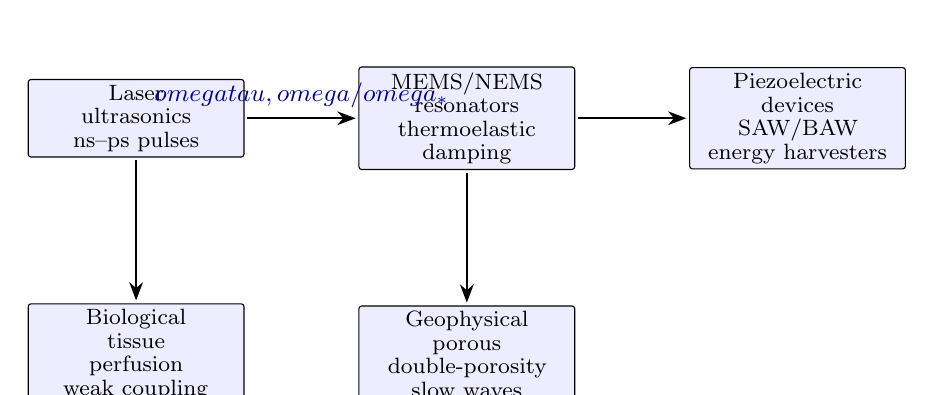
\begin{tikzpicture}[x=1.0cm,y=1.0cm,>=Stealth]
  \tikzset{
    node/.style={draw,rounded corners=1pt,fill=blue!7,align=center,font=\footnotesize,inner sep=2pt,text width=2.6cm},
    arr/.style={->,thick,shorten >=1pt,shorten <=1pt},
    lbl/.style={font=\footnotesize,text=blue!60!black},
  }
  \node[node] at (-3.6, 0.6) (laser) {Laser\\[-1pt] ultrasonics\\[-1pt] ns--ps pulses};
  \node[node] at ( 0.6, 0.6) (res) {MEMS/NEMS\\[-1pt] resonators\\[-1pt] thermoelastic\\[-1pt] damping};
  \node[node] at ( 4.8, 0.6) (piezo) {Piezoelectric\\[-1pt] devices\\[-1pt] SAW/BAW\\[-1pt] energy harvesters};
  \node[node] at (-3.6,-2.4) (bio) {Biological\\[-1pt] tissue\\[-1pt] perfusion\\[-1pt] weak coupling};
  \node[node] at ( 0.6,-2.4) (geo) {Geophysical\\[-1pt] porous\\[-1pt] double-porosity\\[-1pt] slow waves};
  \draw[arr] (laser.east) -- (res.west) node[pos=0.5,above,lbl] {\small $\\omega\\tau,\\omega/\\omega_*$};
  \draw[arr] (res.east) -- (piezo.west) node[pos=0.5,above,lbl] {};
  \draw[arr] (laser.south) -- (bio.north) node[pos=0.5,left,lbl] {};
  \draw[arr] (res.south) -- (geo.north) node[pos=0.5,right,lbl] {};
\end{tikzpicture}

\caption{Application regime map: four areas ordered by the dimensionless numbers $\omega\tau$ (lag relevance) and $\omega/\omega_*$ (coupling relevance); Section~\ref{sec:synthesis} gives the quantitative criteria.}\label{fig:applications-geo}
\end{figure}

\subsection{Summary}
In all four areas the single most informative dimensionless number is $\omega\tau$ (frequency times the relevant lag), and the second is $\omega/\omega_*$. The regime map in Section~\ref{sec:synthesis} makes this quantitative.

\begin{summarybox}[Summary]
Applications divide by regime: laser ultrasonics (classical adequate for ns pulses; lagged/fractional for fs--ps), MEMS/NEMS resonators (Zener damping with nonlocal/lag corrections near cut-off), piezoelectric devices (exact stiffening renormalisation in charge-free regime), biological tissue (weak coupling, interest in thermal field), geophysical porous media (slow diffusive waves, largely untested). The key numbers are $\omega\tau$ and $\omega/\omega_*$.
\end{summarybox}

\section{A quantitative guide to application regimes}\label{sec:scenarios}

\Cref{sec:applications} lists application areas. Here the dimensionless groups that decide the heat law are evaluated for six representative scenarios, so that the reader can see at a glance which of the models of this review is relevant. The table is generated by \path{scripts/table_scenarios.py} from the rounded handbook inputs of \cref{tab:materials} and a lag $\tau_q=1$\,ps; $\delta_T=\sqrt{2\chi/\omega}$ is the thermal penetration depth and $\lambda=c_1/f$ the acoustic wavelength.

\begin{table}[ht]\centering\scriptsize
\caption{Dimensionless groups for six scenarios ($T_0=300$\,K, $\tau_q=1$\,ps). The assessment column applies the rule: Fourier is adequate if $\omega\tau_q<0.1$ and $\omega/\omega_*<0.1$; a lag law may matter if $\omega\tau_q<1.5$ but then the kinetic validity of the model must be checked; otherwise the continuum heat law itself is questionable.}\label{tab:scenarios}
\setlength{\tabcolsep}{3pt}\begin{tabular}{@{}p{3.0cm}lrrrrrp{2.3cm}@{}}\toprule
Scenario & Material & $f$ (Hz) & $\omega/\omega_*$ & $\omega\tau_q$ & $\delta_T$ (m) & $\lambda$ (m) & Assessment\\\midrule
Ultrasonic testing & Aluminium & $1.0\times10^{7}$ & $1.6\times10^{-4}$ & $6.3\times10^{-5}$ & $1.8\times10^{-6}$ & $6.2\times10^{-4}$ & Fourier adequate\\
GHz acoustics & Aluminium & $1.0\times10^{9}$ & $1.6\times10^{-2}$ & $6.3\times10^{-3}$ & $1.8\times10^{-7}$ & $6.2\times10^{-6}$ & Fourier adequate\\
Picosecond ultrasonics & Aluminium & $1.0\times10^{11}$ & $1.6\times10^{0}$ & $6.3\times10^{-1}$ & $1.8\times10^{-8}$ & $6.2\times10^{-8}$ & lag may matter; check kinetics\\
Silicon beam, $h=1\,\mu$m, at $f_Z$ & Silicon & $1.4\times10^{8}$ & $1.1\times10^{-3}$ & $9.1\times10^{-4}$ & $4.5\times10^{-7}$ & $6.1\times10^{-5}$ & Fourier adequate\\
Silicon film, $h=20$\,nm, at $f_Z$ & Silicon & $3.6\times10^{11}$ & $2.7\times10^{0}$ & $2.3\times10^{0}$ & $9.0\times10^{-9}$ & $2.5\times10^{-8}$ & continuum law questionable\\
Copper film, $h=50$\,nm, at $f_Z$ & Copper & $7.3\times10^{10}$ & $2.6\times10^{0}$ & $4.6\times10^{-1}$ & $2.3\times10^{-8}$ & $6.2\times10^{-8}$ & lag may matter; check kinetics\\
\bottomrule\end{tabular}
\end{table}

\subsection{Reading the table}
\begin{itemize}
\item \emph{Ultrasonic testing and GHz acoustics (aluminium).} With $\omega\tau_q$ between $6\times10^{-5}$ and $6\times10^{-3}$ and $\omega/\omega_*$ between $1.6\times10^{-4}$ and $1.6\times10^{-2}$, classical coupled thermoelasticity is adequate. The thermal penetration depth ($1.8\,\mu$m at $10$\,MHz, $0.18\,\mu$m at $1$\,GHz) is much smaller than the acoustic wavelength ($620\,\mu$m and $6.2\,\mu$m), so the wave sees the temperature field as a thin boundary layer at interfaces and as a small bulk damping.
\item \emph{Picosecond ultrasonics (aluminium, 100\,GHz).} Here $\omega/\omega_*=1.6$ and $\omega\tau_q=0.63$ and the wavelength ($62$\,nm) is comparable with the thermal penetration depth ($18$\,nm). This is the regime of the regime map (\cref{sec:synthesis}) where lag and coupling effects could be visible, and also where carrier mean free paths are comparable with the wavelength, so the interpretation of any deviation from the classical result requires a kinetic or atomistic cross-check.
\item \emph{Silicon beam, $h=1\,\mu$m.} At the Zener frequency $f_Z=1.4\times10^{8}$\,Hz, $\omega\tau_q\approx10^{-3}$ and the Fourier law with the exact flexural result \cref{eq:LR} is adequate. The thermal penetration depth ($0.45\,\mu$m) is a sizeable fraction of the thickness, which is why the damping peaks here.
\item \emph{Silicon film $20$\,nm and copper film $50$\,nm.} At the thermal relaxation frequency of the film, $\omega\tau_q$ is $2.3$ and $0.46$ and $\omega/\omega_*$ is $2.7$ and $2.6$. These are the regimes in which a continuum heat law with bulk parameters has to be treated with caution: the film thickness is comparable to or below the carrier mean free path, boundary scattering reduces the effective conductivity, and the relaxation frequency of the continuum model is not reliable.
\end{itemize}

\subsection{Consequences for the choice of theory}
\begin{enumerate}
\item The classical coupled theory suffices for essentially all ultrasonic, MEMS-scale-above-micron and geophysical-scale applications, and it is the one to use as a baseline in any case.
\item Lag models can only matter in the lower right-hand corner of \cref{tab:scenarios}: frequencies above about $10^{10}$\,Hz or thicknesses below about $100$\,nm. In that corner the continuum assumptions are also stressed, so any claim of a lag effect needs an independent test.
\item The Guyer--Krumhansl and nonlocal models (\cref{sec:kinetic,sec:size}) are the first refinement once size effects are suspected, because they carry a length scale; lag models do not.
\item The electromechanical and magnetic couplings (\cref{sec:multi}) change the stiffness at all frequencies, and are therefore relevant over the whole table, even where the heat law is not.
\end{enumerate}

\section{Worked examples}\label{sec:examples}

This section shows how the results of the review are used for four practical questions. All numbers follow from the rounded handbook inputs of \cref{tab:materials} at $T_0=300$\,K (script \path{scripts/worked_examples.py}); they illustrate the procedure and should be redone with measured parameters for a specific specimen.

\subsection{Example 1: Does a lag law matter for ultrasound in aluminium?}
\textbf{Question.} A 1\,GHz longitudinal wave propagates in aluminium; should a Cattaneo (Lord--Shulman) law with $\tau_q=1$\,ps be used instead of Fourier's law?

\textbf{Step 1: characteristic numbers.} From \cref{tab:materials}: $c_1=6198$\,m/s, $\varepsilon=0.027$, $\omega_*=\rho c c_1^2/k=3.94\times10^{11}$\,rad/s. The lag enters through $\tau_q\omega_*=0.39$, so the thermal front speed $c_T=\sqrt{k/(\rho c\tau_q)}=9.9$\,km/s is $1.6\,c_1$.

\textbf{Step 2: where the wave sits on the dispersion curves.} At $1$\,GHz the frequency ratio is $\omega/\omega_*=1.6\times10^{-2}$ and $\omega\tau_q=6.3\times10^{-3}$. The Debye loss of \cref{eq:debye} is $Q^{-1}=\varepsilon x/(1+x^2)=4.3\times10^{-4}$ with $x=\omega/\omega_*$; at $1$\,MHz it is $4.3\times10^{-7}$.

\textbf{Step 3: what the lag changes.} The lag modifies the response through $\omega\tau_q$. By the truncation analysis of \cref{sec:delayfid} the corrections to the thermal branch are at the $10^{-4}$ level or below for $\omega\tau_q\sim6\times10^{-3}$ (the first-order relative error scales as $(\omega\tau)^2/4$), so the Fourier result is adequate. The lag would matter only at frequencies of order $\omega_*$ or above, i.e.\ tens of GHz, where in addition the phonon mean free path is comparable with the wavelength and the kinetic closure of \cref{sec:kinetic} is not valid.

\textbf{Conclusion.} For ultrasonic and MHz--GHz applications in aluminium the parabolic (Biot) theory is the correct model, and a lag law adds parameters without adding accuracy.

\subsection{Example 2: Thermoelastic damping of a silicon nanobeam}
\textbf{Question.} At which frequency does the thermoelastic loss peak for a silicon beam of thickness $h$, and how large is it?

\textbf{Step 1.} The diffusivity is $\chi=k/\rho c=9.2\times10^{-5}$\,m$^2$/s. The Zener frequency is $f_Z=\pi\chi/(2h^2)$, which gives $1.4\times10^{6}$\,Hz for $h=10\,\mu$m, $1.4\times10^{8}$\,Hz for $1\,\mu$m, $1.4\times10^{10}$\,Hz for $100$\,nm and $3.6\times10^{9}$\,Hz for $h=200$\,nm (a value in between).

\textbf{Step 2.} The relaxation strength is $\Delta=E\alpha_T^2T_0/c_v=2.0\times10^{-4}$, so the peak loss is $Q^{-1}_{\max}\approx0.494\,\Delta\approx1.0\times10^{-4}$ (\cref{sec:flexted}). This corresponds to a quality factor limit of about $10^{4}$ at the peak, which is a significant limit for sub-micron resonators with intrinsic $Q$ above $10^{4}$.

\textbf{Step 3: check validity.} A micron-size silicon beam at $f_Z\sim10^{8}$\,Hz has $\omega\tau_q\sim10^{-3}$ for $\tau_q\sim1$\,ps, so a lag law is not required. For $h\lesssim100$\,nm, bulk values of $k$ are no longer reliable because the phonon mean free path in silicon at room temperature (hundreds of nanometres) exceeds the thickness, and the Guyer--Krumhansl or kinetic description (\cref{sec:kinetic}) is the relevant model, with a thickness-dependent effective conductivity as input.

\subsection{Example 3: Energy partition at an aluminium--copper interface}
\textbf{Question.} What fraction of a normally incident longitudinal wave in aluminium is reflected at a welded copper interface (elastic limit)?

The impedances are $Z_1=\rho c_1=1.67\times10^{7}$ and $Z_2=4.07\times10^{7}$\,kg\,m$^{-2}$s$^{-1}$ (aluminium, copper). Then $r=(Z_1-Z_2)/(Z_1+Z_2)=-0.417$, $t=2Z_1/(Z_1+Z_2)=0.583$, $R=r^2=0.174$ and $T=(Z_2/Z_1)t^2=0.826$, with $R+T=1$ to four digits. The sign of $r$ shows a phase reversal of the reflected displacement wave (impedance increases). When thermal coupling is included, the reflected and transmitted amplitudes acquire corrections of order $\varepsilon$ and additional thermal waves are generated; the energy bookkeeping must use the net-flux conservation of \cref{sec:interfaces}, not the sum of mode-wise energy fractions.

\subsection{Example 4: Is a heat pulse in steel hyperbolic?}
\textbf{Question.} A surface of steel is heated at $t=0$. After how long does the Fourier and the Cattaneo solution differ, and by how much in position?

For steel $\chi=1.3\times10^{-5}$\,m$^2$/s. The Fourier diffusion length is $\sqrt{\chi t}=1.1\times10^{-7}$\,m at $t=1$\,ns and $3.6\times10^{-6}$\,m at $1\,\mu$s. The Cattaneo front speed for $\tau_q=1$\,ps is $\sqrt{\chi/\tau_q}=3.6$\,km/s, so the front has travelled only $3.6\times10^{-9}$\,m in one lag time. The two solutions therefore differ only for $t\lesssim$ a few $\tau_q$ and within a few nanometres of the surface, where continuum theory and a bulk $k$ are already questionable. Resolving the difference requires a time resolution well below a picosecond, so any such experiment needs ultrashort-pulse (sub-picosecond) heating and detection.

\subsection{Lessons}
(i) Compute $\omega_*$, $\varepsilon$ and $\omega\tau_q$ before choosing a model; the regime map of \cref{sec:synthesis} shows at a glance whether lag effects can matter. (ii) For devices below about $100$\,nm the first deviation from the Fourier picture is size-related, not lag-related. (iii) The elastic interface calculation is a necessary baseline for the thermoelastic one.

\section{Experimental evidence and parameter identification}\label{sec:experiments}

A theory of wave propagation is only as useful as its parameters. This section reviews which experiments probe which model parameters, what they can and cannot discriminate, and how to read published values of lag times and fractional orders.

\subsection{Second sound and ballistic heat pulses}
The direct signature of wave-like heat transport is second sound, a propagating temperature wave. It was predicted for dielectric crystals at low temperature \citep{Chester1963,GuyerKrumhansl1966} and observed in solid helium \citep{Ackerman1966} and in sodium fluoride \citep{McNelly1970,Jackson1970}, in narrow temperature windows where momentum-conserving phonon collisions dominate over resistive ones. A further observation in graphite above $100$\,K \citep{Huberman2019} extends the window to a much higher temperature in a material of high anisotropy. The conditions of these experiments, a hydrodynamic phonon window with $\tau_N\ll\tau_R$, are exactly those under which the Guyer--Krumhansl law (\cref{sec:kinetic}) is the appropriate description. They do not demonstrate that a Cattaneo or lag law with a single relaxation time describes heat conduction in common solids at room temperature.

\subsection{Ultrafast optical methods}
Pump--probe reflectivity measures electron--lattice energy exchange on femtosecond to picosecond timescales \citep{Brorson1987} and picosecond ultrasonics generates and detects coherent acoustic pulses in thin films \citep{Thomsen1986}. In the first, the two-temperature picture of \cref{sec:lags} is the relevant continuum model, and the measured quantity is an electron--phonon coupling time rather than $\tau_q$. In the second, the heat input launches a strain pulse whose amplitude and shape depend on the thermal diffusion within the first tens of nanometres; thermoelastic coupling is then the source, not a loss mechanism. Time-domain thermoreflectance \citep{Cahill2003} extracts the conductivity of films and interfaces by fitting a diffusive model with interface resistance, and a deviation from that model at short delay is the usual place where a lag or ballistic correction is claimed.

\subsection{Resonator quality factors}
Micro- and nano-resonators provide the cleanest tests of thermoelastic damping because $Q$ can be measured against temperature and thickness. The quantitative signature, \cref{eq:zenerQ,eq:LR}, is a loss peak at $f_Z=\pi\chi/(2h^2)$ with the scaling $f_Z\propto h^{-2}$ and a height proportional to $\Delta$. Verification therefore requires a sweep of thickness or temperature and not a single value, and requires subtracting anchor and surface losses, which are not described by the models of this review. A mismatch can be attributed to a lag or size effect only when these contributions have been bounded.

\subsection{Heterogeneous media and biological tissue}
The relaxation times $\tau_q$ of order seconds reported for non-homogeneous materials, including processed biological tissue \citep{Mitra1995,Kaminski1990}, reflect heat transfer through a heterogeneous microstructure and are effective macroscopic parameters. Their interpretation as a molecular relaxation time is not warranted, and the observed values have been disputed in the literature. For tissue the parabolic Pennes bioheat equation \citep{Pennes1948} remains the baseline against which any hyperbolic correction must be assessed.

\subsection{How to read a published lag time}
\begin{enumerate}
\item Identify what was measured: a response time of a temperature signal, a conductivity, or a quality factor.
\item Identify the model used to extract $\tau$ and whether other parameters were fitted simultaneously. A fit of two or more lag parameters from a single curve is usually not identifiable (compare \cref{sec:delayfid}).
\item Compare $\omega\tau$ with the validity limits of the model (\cref{sec:delayfid} for truncated lag laws, \cref{sec:kinetic} for the kinetic basis).
\item Check whether a simpler model (Fourier with interface resistance, or Guyer--Krumhansl) explains the same data.
\end{enumerate}
A model parameter that cannot be measured independently of the model that defines it is a fitting constant and not a material property, and papers that tabulate such constants for many materials without an independent test provide limited guidance.

\begin{summarybox}[Summary]
Experimental evidence: second sound at cryogenic temperatures (Ackerman--Bertman, Jackson et al.) is the cleanest demonstration of wave-like heat transport; room-temperature reports of large relaxation times in nonhomogeneous materials are debated. Pump--probe and ultrasonic damping can determine lags independently. A model parameter not measurable independently of the model is a fitting constant, not a material property.
\end{summarybox}

\section{Comparative synthesis and decision guide}\label{sec:synthesis}
\subsection{When does the heat law matter? A regime map}
The question that most users face is whether a generalized heat law will change their prediction. We answer it for the damping and speed of the elastic-type branch by computing the relative difference between Lord--Shulman and classical predictions over the plane of the two relevant dimensionless numbers, the frequency $\omega/\omega_*$ and the lag $\tau_0\omega_*$ (\Cref{fig:regime}). The coupling is taken as $\varepsilon=0.02$, typical of metals (Table~\ref{tab:materials}).
\begin{figure}[t]\centering
\includegraphics[width=\textwidth]{figs/fig_regime_map.pdf}
\caption{Relative difference between the Lord--Shulman and classical predictions for the elastic-type branch ($\varepsilon=0.02$): (a) damping $Q^{-1}$, (b) phase speed. Dashed and solid white contours mark $1\,\%$ and $10\,\%$ differences; the dotted red line is $\omega\tau_0=1$. Near $\tau_0\omega_*\approx1$ the thermal and elastic speeds coincide ($c_T=c_1$), the branches hybridise, and the labelling ``elastic-type'' is ambiguous; features in that region should be read qualitatively.}\label{fig:regime}
\end{figure}
Three conclusions can be read off. (i) The heat law affects the \emph{damping} much earlier than the \emph{speed}: a $10\,\%$ change in $Q^{-1}$ at $\omega\gtrsim\omega_*$ requires $\omega\tau_0\gtrsim0.05$--$0.1$, and a $1\,\%$ change requires roughly $\omega\tau_0\gtrsim0.005$, whereas the phase speed changes by less than $1\,\%$ over most of the plane. (ii) At frequencies far below $\omega_*$ the difference is negligible unless the lag is very large, because the thermal field is then adiabatic over a period. (iii) In the neighbourhood of $\omega\tau_0=1$ differences of tens of percent in $Q^{-1}$ appear. Consequently, a paper that reports a ``strong effect of the relaxation time on the phase speed'' for realistic lags and ultrasonic frequencies should be examined for the choice of nondimensionalisation: a nondimensional lag chosen for plotting convenience can be far larger than any physical value.

\subsection{Taxonomy of models and combinations}
\Cref{tab:taxonomy} places the models discussed in this review according to the structure of their heat law (the function $G(s)$), the elastic constitutive law, and the additional fields. A published model is a point in the product of these three choices; the number of models in the literature is large because the product is large, not because there are many physically distinct mechanisms.
\begin{table}[ht]\centering\small
\caption{Taxonomy. A model is specified by one entry from each of the three groups.}\label{tab:taxonomy}
\begin{tabularx}{\textwidth}{@{}p{2.6cm}X@{}}\toprule
Axis & Options (representative references)\\\midrule
Heat law $G(s)$ & Fourier \citep{Biot1956}; Cattaneo/LS \citep{Lord1967}; Green--Lindsay (modifies coupling) \citep{Green1972}; GN I--III \citep{Green1991,Green1993}; DPL \citep{Tzou1995}; TPL \citep{RoyChoudhuri2007}; MGT \citep{Quintanilla2019}; fractional \citep{Povstenko2016}; MDD \citep{Wang2011}; Guyer--Krumhansl \citep{GuyerKrumhansl1966II}; two-temperature variants \citep{Youssef2006}.\\
Elastic law & Local; Eringen nonlocal \citep{Eringen1972,Eringen1974}; gradient \citep{Aifantis1992,Askes2011}; couple stress \citep{MindlinTiersten1962}; micropolar \citep{Eringen1999}; Klein--Gordon type \citep{Lazar2022}; viscoelastic (Kelvin--Voigt) \citep{Gupta2026HeatMap}.\\
Added fields & Piezoelectric \citep{Mindlin1974Thermopiezo}; semiconductor/photothermal \citep{Gupta2023}; magnetic \citep{Ezzat2011}; diffusion \citep{Abouelregal2020a}; voids/porosity \citep{Cowin1983,Iesan1986,Singh2020}.\\\bottomrule
\end{tabularx}
\end{table}

\subsection{Comparative table}
\Cref{tab:final} summarises the models along the criteria that determine when each is appropriate.
\begin{table}[ht]\centering\small
\caption{Comparative summary of heat-conduction models for thermoelastic waves.}\label{tab:final}
\begin{tabularx}{\textwidth}{@{}p{2.3cm}p{1.5cm}p{1.9cm}p{2.3cm}X@{}}\toprule
Model & Extra parameters & Finite front speed & Well-posed when & Main caution\\\midrule
Classical & 0 & no & always & Instantaneous thermal signal.\\
Lord--Shulman & 1 ($\tau_0$) & yes ($c_T$) & $\tau_0>0$ & Lag also multiplies the coupling term.\\
Green--Lindsay & 2 ($\tau_0,\tau_1$) & yes & $\tau_0\ge\tau_1\ge0$ & Discontinuities at fronts.\\
GN II & 1 ($k^*$) & yes ($c_*$) & $k^*>0$ & No dissipation.\\
GN III & 2 ($k,k^*$) & no (strict) & both $>0$ & Not an improved Cattaneo law.\\
DPL, 1st order & 2 & no (strict) & no instability found numerically & Both-limits diffusive; $\tau_T=\tau_q$ is Fourier.\\
DPL, 2nd order in $\tau_q$ & 2 & depends & $\tau_T\ge\tau_q/2$ & Ill-posed otherwise.\\
TPL & 4 & no (strict) & see \citep{Chirita2016} & Many parameters; $k^*$ changes low-$\omega$ limit.\\
MGT & 2--3 & yes ($c_T$) & parameter conditions & Third order in time.\\
Fractional & 1 order + lag & depends on $\alpha$ & model-dependent & $\alpha\to2$ is not Fourier.\\
MDD & 1--3 & variant-dependent & model-dependent & High-frequency limit depends on kernel.\\\bottomrule
\end{tabularx}
\end{table}

\subsection{Pitfalls checklist}
The following issues occur repeatedly in the literature and were each examined in this review.
\begin{enumerate}
\item \textbf{The $\tau_T\ge\tau_q/2$ condition belongs to the second-order-in-$\tau_q$ truncation} of DPL, not to the first-order template; the first-order version is stable for all $\tau_T>0$ (Section~\ref{sec:lags}).
\item \textbf{DPL $\to$ Lord--Shulman} needs $\tau_T\to0$ at fixed $\tau_q$, not $\tau_q\to0$; $\tau_T=\tau_q$ gives exactly Fourier's law.
\item \textbf{TPL $\to$ DPL} needs $k^*\to0$; with $k^*\ne0$ the low-frequency limit changes qualitatively.
\item \textbf{Fractional order $\alpha\to2$ is the wave equation, not Fourier's law.}
\item \textbf{GN-III does not have a finite thermal front speed}; it is wave-like at low and diffusive at high frequency.
\item \textbf{The classical theory is adiabatic at low and isothermal at high frequency}; labels on speeds must say which modulus $c_1$ refers to.
\item \textbf{Branch identification}: follow roots by continuity; nearest-to-$\omega/c_1$ selection fails when branches hybridise.
\item \textbf{DPL is diffusive at both ends}; ``wave-like'' only at intermediate frequency.
\item \textbf{The sign of the effect of a hyperbolic heat law on a pulse depends on the boundary condition} (prescribed flux or temperature).
\item \textbf{MDD forms differ in their high-frequency limit}; check $s\kappa(s)$ as $s\to\infty$.
\item \textbf{Energy ratios in lossy media}: the sum of mode fractions need not equal one because of interference; the net flux must be continuous.
\item \textbf{Eringen calibration}: $\xi$ depends on the calibration target (zone boundary versus long wavelength).
\item \textbf{Gradient sign}: a positive gradient coefficient gives stiffening dispersion, the opposite of lattice softening.
\item \textbf{Nonlocal thermoelastic form} (smoothing the thermal stress or not) changes damping near the cut-off.
\item \textbf{Talbot inversion fails for delayed transforms} for times before the delay; set the solution to zero ahead of the front.
\item \textbf{Piezo sign conventions}: the sign of $ep$ determines whether pyroelectricity increases or decreases thermal stress.
\item \textbf{Report dimensionless groups} so that nondimensional lags can be related to physical values.
\end{enumerate}

\subsection{Decision guide}
\Cref{fig:guide} gives a decision sequence for choosing a starting model. It is a guide, not a substitute for checking against data.
\begin{figure}[t]\centering
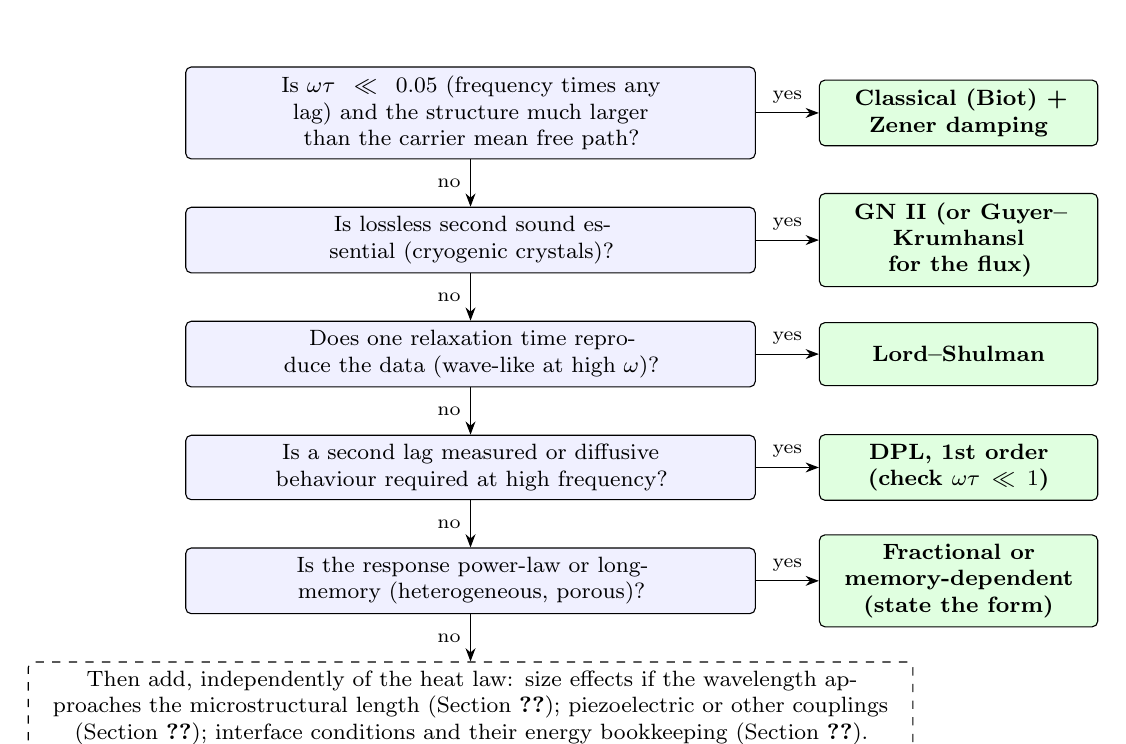
\begin{tikzpicture}[
 node distance=6mm and 8mm,
 q/.style={draw,rounded corners=2pt,fill=blue!6,align=center,font=\footnotesize,text width=7.0cm,minimum height=8mm},
 a/.style={draw,rounded corners=2pt,fill=green!12,align=center,font=\footnotesize\bfseries,text width=3.3cm,minimum height=8mm},
 >=Stealth]
\node[q] (q1) {Is $\omega\tau\ll0.05$ (frequency times any lag) and the structure much larger than the carrier mean free path?};
\node[a,right=of q1] (a1) {Classical (Biot) + Zener damping};
\node[q,below=of q1] (q2) {Is lossless second sound essential (cryogenic crystals)?};
\node[a,right=of q2] (a2) {GN II (or Guyer--Krumhansl for the flux)};
\node[q,below=of q2] (q3) {Does one relaxation time reproduce the data (wave-like at high $\omega$)?};
\node[a,right=of q3] (a3) {Lord--Shulman};
\node[q,below=of q3] (q4) {Is a second lag measured or diffusive behaviour required at high frequency?};
\node[a,right=of q4] (a4) {DPL, 1st order (check $\omega\tau\ll1$)};
\node[q,below=of q4] (q5) {Is the response power-law or long-memory (heterogeneous, porous)?};
\node[a,right=of q5] (a5) {Fractional or memory-dependent (state the form)};
\draw[->] (q1)--(a1) node[midway,above,font=\scriptsize]{yes};
\draw[->] (q1)--(q2) node[midway,left,font=\scriptsize]{no};
\draw[->] (q2)--(a2) node[midway,above,font=\scriptsize]{yes};
\draw[->] (q2)--(q3) node[midway,left,font=\scriptsize]{no};
\draw[->] (q3)--(a3) node[midway,above,font=\scriptsize]{yes};
\draw[->] (q3)--(q4) node[midway,left,font=\scriptsize]{no};
\draw[->] (q4)--(a4) node[midway,above,font=\scriptsize]{yes};
\draw[->] (q4)--(q5) node[midway,left,font=\scriptsize]{no};
\draw[->] (q5)--(a5) node[midway,above,font=\scriptsize]{yes};
\node[draw,dashed,rounded corners=2pt,font=\footnotesize,below=of q5,text width=11cm,align=center] (add) {Then add, independently of the heat law: size effects if the wavelength approaches the microstructural length (Section~\ref{sec:size}); piezoelectric or other couplings (Section~\ref{sec:multi}); interface conditions and their energy bookkeeping (Section~\ref{sec:interfaces}).};
\draw[->] (q5)--(add) node[midway,left,font=\scriptsize]{no};
\end{tikzpicture}
\caption{Decision sequence for choosing a starting model. The threshold $\omega\tau\ll0.05$ follows from the regime map of \Cref{fig:regime}.}\label{fig:guide}

\begin{summarybox}[Summary]
Comparative synthesis: all template models share one dispersion polynomial; differences show in damping before speed and only when $\omega\tau\gtrsim0.05$. LS and MGT have finite thermal fronts; classical, DPL, TPL and GN-III do not (first-order template). GN-II is unique in being energy-conserving. Piezoelectric stiffening is exact in the charge-free regime. Nonlocal lengths are calibration-dependent. At interfaces in lossy media, net flux is conserved but mode fractions need not sum to one.
\end{summarybox}
\end{figure}

\section{Reporting standards for new work}\label{sec:reporting}

The comparisons made in this review were often limited not by the models but by what the original papers report. This section proposes a short set of reporting standards that would make future results directly comparable. They follow from the pitfalls collected in \cref{sec:synthesis} and from the checks of \cref{sec:methods,sec:schemes}.

\subsection{What a paper on generalized thermoelastic waves should state}
\begin{enumerate}
\item \textbf{The heat-flux law as an explicit parameter set.} Give the model in the template of \cref{sec:foundations} (or state where it departs from it) so that $G(s)$, the polynomial of \cref{eq:unified} and the limit $\omega\to\infty$ follow without reading the derivation. For lagging models give the truncation order.
\item \textbf{Which limits were verified.} State the reductions that were tested numerically or symbolically, for example Fourier, Lord--Shulman and the elastic limit $\varepsilon\to0$, and give the numerical agreement achieved.
\item \textbf{A non-dimensional parameter table.} Report $\varepsilon$, $\omega/\omega_*$, $\omega\tau_q$ (and $\omega\tau_T$, $\alpha$, $\xi\omega_*/c_1$ as relevant) for every figure. A figure for which these are not given cannot be placed on the regime map of \cref{sec:synthesis}.
\item \textbf{The material source and the status of the parameters.} Say whether a lag time or fractional order is measured, estimated by a stated argument, or assigned for illustration. Illustrative values should not be presented in a table with measured ones.
\item \textbf{Branch handling.} For dispersion curves state how roots were selected and followed (\cref{sec:prelim}), and mark regions of hybridisation.
\item \textbf{Energy statements.} If energy ratios are reported, give the energy flux used (\cref{sec:energy}), state whether the ratios sum to one, and if they do not, whether the cross terms between modes were included (\cref{sec:interfaces}).
\item \textbf{Inversion and discretisation.} For transient results state the Laplace-inversion method and the cross-check, or the discretisation and Courant number, and give the error in a window around the front separately from the global error (\cref{sec:schemes}).
\item \textbf{Boundary and interface conditions.} State the thermal condition (insulated, isothermal, convective) and, at interfaces, the continuity conditions for the heat flux and for the temperature or the thermal displacement.
\end{enumerate}

\subsection{Claims that need an independent test}
\begin{itemize}
\item A lag time or fractional order extracted from a single curve with several free parameters.
\item A statement that a model predicts a ``new wave'' without a check of the number of roots of the dispersion polynomial in each frequency range and of their causality (\cref{sec:prelim}).
\item A reflection or transmission result that agrees with an energy ratio sum of one only because the thermal wave has been dropped.
\item A size effect obtained from a nonlocal law whose length parameter has been chosen by trial rather than calibrated to a lattice or atomistic dispersion curve (\cref{sec:size}).
\end{itemize}

\subsection{Limitations of this review}
The review treats linear waves about a uniform reference state and does not cover nonlinear thermoelasticity, radiative or reactive heat transfer, or the full literature on bounded-domain well-posedness. The numerical checks use rounded handbook values and non-dimensional parameter sets chosen to separate the effects discussed; they illustrate mechanisms and should be repeated with measured parameters before being used for design. The classified catalogue in the appendix is organised by title keywords and does not assess the content of the individual papers. Statements that rest on the cited literature rather than on the computations reported here are identified by their citations.

\section{Open problems and research agenda}\label{sec:open}
\subsection{Theory}
\begin{enumerate}
\item \textbf{A classification theorem for the template.} For the first-order template we have shown numerically that DPL is stable for all positive lags and identified when the thermal front has finite speed (the behaviour of $sG(s)$ at large $s$). A complete analytical statement of well-posedness, decay and front structure for the coupled TPL and MGT systems with all parameters positive, including the conditions on $(\tau_q,\tau_T,\tau_v,k,k^*)$ and the role of the coupling $\varepsilon$, is still lacking in a form directly usable by applied authors.
\item \textbf{Thermodynamics of truncated lag models.} The time-differential DPL and TPL models raise questions of thermodynamic compatibility and continuous dependence \citep{Chirita2016,Tibullo2017}; a systematic account of which truncations admit an energy functional and entropy inequality, and what restrictions this imposes on the lags, would resolve the confusion about the $\tau_T\ge\tau_q/2$ condition (Section~\ref{sec:lags}).
\item \textbf{Memory-dependent and fractional models.} Energy functionals, thermodynamic admissibility, uniqueness and finite-speed properties for the memory-dependent and fractional laws are not available in the generality of the template models. The high-frequency limit of the MDD law, which depends on the kernel (Section~\ref{sec:memory}), suggests that a classification of kernels by $s\kappa(s)$ at large $s$ would be valuable.
\item \textbf{Interface conditions for lagged and memory models.} Thermodynamically consistent interface conditions with thermal resistance, for lagged and memory heat laws, including the entropy production at the interface (Section~\ref{sec:interfaces}).
\item \textbf{Mode interference in dissipative media.} A systematic framework for apportioning energy flux among generated waves in lossy media, so that energy ratios have an unambiguous meaning.
\end{enumerate}
\subsection{Combined effects}
\begin{enumerate}
\setcounter{enumi}{5}
\item \textbf{Joint size and memory effects.} Combinations of nonlocal or gradient elasticity with hyperbolic or memory heat laws are widely computed but rarely validated against lattice dynamics or atomistic simulation. A benchmark in which a lattice model with heat carriers supplies the reference dispersion would show which combination is justified.
\item \textbf{Calibration of length scales.} The calibration target (zone boundary versus long wavelength) changes $\xi$ by about one third (Section~\ref{sec:size}); systematic calibration protocols for thermoelastic problems are missing.
\item \textbf{Nonlocal forms of thermoelastic coupling.} The two forms (smoothed or unsmoothed thermal stress) differ near the cut-off; the thermodynamically consistent form should be derived from a nonlocal free energy.
\item \textbf{Surface and interface thermoelasticity at the nanoscale.} Surface stress, surface heat capacity and Kapitza resistance modify both surface waves and interface partition in ways not captured by the bulk models treated here.
\end{enumerate}
\subsection{Experiments and data}
\begin{enumerate}
\setcounter{enumi}{9}
\item \textbf{Measurement of both branches.} Experiments that measure the elastic-type and the thermal-type branch in the same solid across the crossover frequency would discriminate among heat laws; at present most evidence is indirect.
\item \textbf{Independent determination of lags.} The relaxation times and lags are generally obtained by fitting; independent measurement (for example from pump--probe experiments together with ultrasonic damping) would allow a test of the models rather than a fit.
\item \textbf{Thermoelastic damping at ultra-high frequency.} Resonators operating at gigahertz frequencies reach the regime where lagged corrections matter; systematic data on damping versus frequency and size would calibrate them.
\end{enumerate}
\subsection{Computation}
\begin{enumerate}
\setcounter{enumi}{12}
\item \textbf{Benchmark suite.} A set of agreed benchmark problems (the heat pulse, thermal shock, Rayleigh wave and interface problems of this review) with reference solutions at specified precision would improve the reliability of numerical codes.
\item \textbf{Efficient memory operators.} Fast algorithms for fractional and memory-dependent operators in time-domain codes, with error control.
\end{enumerate}

\section{Conclusions}\label{sec:conclusions}
Generalized thermoelasticity is not a collection of unrelated theories but a family organised by the function $G(s)$ that relates heat flux to temperature gradient, combined with choices of elastic law and added fields. This organisation makes three kinds of result possible. First, exact statements about reductions and limits, including a clarification that the often-quoted DPL stability condition belongs to a specific truncation and that GN-III has no finite front speed. Second, a single dispersion polynomial that gives comparative speeds, attenuation and thermoelastic damping, and that shows that the heat law affects damping long before it affects speed, and only for $\omega\tau\gtrsim0.05$. Third, problem-level insights: finite fronts and surface jumps in heat pulses, the structure of thermoelastic Rayleigh waves, the renormalisation by piezoelectric coupling, calibration dependence of nonlocal lengths, and the distinction between net energy flux and mode-by-mode fractions at interfaces in lossy media. Many of the open questions concern validation rather than derivation: independent measurement of lags, joint validation of size and memory effects against lattice dynamics, and benchmark solutions. We hope that the unified notation, the verified reductions, the pitfalls checklist and the decision guide help readers choose, justify and check models, and that the open problems direct effort where it is most needed.

\appendix
\section{Derivation and verification of the dispersion polynomial}\label{app:disp}
With $\partial_x\to\ii k$ and $\partial_t\to s=-\ii\omega$, the momentum and energy balances \eqref{eq:1d} for the template give the linear system
\begin{align}
\bigl(\rho s^2+\rho c_1^2k^2\bigr)\hat u+\ii\beta k\,\hat\theta&=0,\\
T_0\beta\,s\,\ii k\,\hat u+\bigl(s\rho c+G(s)k^2\bigr)\hat\theta&=0,
\end{align}
where the second equation uses $\ii k\,\hat q=-\ii k\,G\,\ii k\,\hat\theta=Gk^2\hat\theta$. Its determinant is
$(\rho c_1^2k^2+\rho s^2)(s\rho c+Gk^2)+\beta^2T_0\,s\,k^2$ (since $(\ii k)(\ii k)=-k^2$), which is \eqref{eq:disp} because $\rho s^2=-\rho\omega^2$. The identity was checked symbolically with all template parameters kept as symbols (script \path{check_dispersion.py}); a first version of our own implementation had the opposite sign for the coupling term, and the symbolic comparison detected it immediately, which is the reason we advocate the check.

\paragraph{Unified form for LS and GL.} Multiplying by $1+\tau_0s$ for $G=k/(1+\tau_0s)$ gives \eqref{eq:unified} with $\tau^\dagger=\tau_0$; the Green--Lindsay system of \eqref{eq:GL} gives the same polynomial with $\tau^\dagger=\tau_1$, since the thermal-stress term carries $(1+\tau_1s)$.

\paragraph{Limits.} Setting $\beta\to0$ decouples the roots into $K=-s^2/c_1^2$ and $K=-s\rho c/G$; for $G=k$ the latter is $k^2=\ii\omega/\alpha$ with phase speed $\sqrt{2\alpha\omega}$.

\paragraph{Nonlocal forms.} If the stress law is $(1-\xi^2\partial_x^2)\sigma=c\,u_{,x}-\beta\theta$ (form A of Section~\ref{sec:size}), the momentum balance becomes $[\rho s^2(1+\xi^2K)+\rho c_1^2K]\hat u+\ii\beta k\hat\theta=0$ and the determinant is $[\rho s^2(1+\xi^2K)+\rho c_1^2K](s\rho c+GK)+\beta^2T_0sK=0$; for form B the last term is multiplied by $1+\xi^2K$.

\section{Characteristic numbers and parameter estimates}\label{app:numbers}
For a given solid and a given heat-flux model, the dimensionless groups that control the problem are collected in \Cref{tab:groups}.
\begin{table}[ht]\centering\small
\caption{Dimensionless groups for thermoelastic wave problems.}\label{tab:groups}
\begin{tabular}{@{}llp{6.2cm}@{}}\toprule
Group & Definition & Meaning\\\midrule
$\varepsilon$ & $\beta^2T_0/(\rho^2cc_1^2)$ & adiabatic--isothermal modulus difference\\
$\omega_*$ & $\rho cc_1^2/k$ & frequency at which conduction over a wavelength matches the period\\
$\omega\tau$ & $\omega\tau_q$ & frequency times flux lag\\
$c_T/c_1$ & $\sqrt{k/(\rho c\tau_0)}/c_1=1/\sqrt{\tau_0\omega_*}$ & thermal-to-elastic front speed\\
$\tau_T/\tau_q$ & & lag ratio (DPL)\\
$\xi\omega_*/c_1$ & & nonlocal length in thermal units\\
$K^2$ & $e^2/(\varepsilon_ec)$ & electromechanical coupling\\
\bottomrule\end{tabular}
\end{table}
Note that $c_T/c_1=1/\sqrt{\tau_0\omega_*}$: the thermal front is faster than the elastic one for $\tau_0\omega_*<1$ and slower for $\tau_0\omega_*>1$, and branch hybridisation occurs at $\tau_0\omega_*\approx1$ (\Cref{fig:regime}). With the values of Table~\ref{tab:materials} and a lag time of one picosecond, $\tau_0\omega_*\approx0.4$ for aluminium, i.e.\ a thermal front somewhat faster than the elastic one.

\section{Reproducibility: scripts and what each one verifies}\label{app:repro}
All numerical results of this review are produced by Python scripts supplied with the manuscript. \Cref{tab:scripts} lists them with the checks they perform.
\begin{table}[ht]\centering\small
\caption{Scripts and the identities or limits they verify.}\label{tab:scripts}
\begin{tabularx}{\textwidth}{@{}p{4.2cm}X@{}}\toprule
Script & Content and checks\\\midrule
\path{check_dispersion.py} & Symbolic determinant of the field equations equals the dispersion polynomial \eqref{eq:disp} (difference zero).\\
\path{check_reductions.py} & Reductions of $G(s)$: DPL$\to$LS, TPL$\to$DPL, GN-II/III, large-$s$ limits.\\
\path{check_fronts.py} & LS and GL front speeds from the polynomial agree with \eqref{eq:fronts} to four digits.\\
\path{check_gn2.py} & GN-II speeds are non-dispersive and equal the formula.\\
\path{check_thermopiezo.py} & Thermopiezoelectric determinant is proportional to the renormalised thermoelastic polynomial \eqref{eq:renorm}.\\
\path{fig_dispersion.py}, \path{fig_zener_q.py} & Dispersion and damping; weak-coupling Debye result confirmed ($Q^{-1}/\varepsilon=0.4999998$).\\
\path{fig_stability.py} & Growth rates for the 1st- and 2nd-order DPL truncations.\\
\path{fig_heatpulse.py} & Cattaneo pulse by Talbot inversion; Fourier limit and front exactness.\\
\path{fig_shock.py} & Thermal shock of a coupled half-space; boundary conditions satisfied to machine precision.\\
\path{fig_rayleigh.py} & Thermoelastic Rayleigh root; $\varepsilon\to0$ limit gives the elastic Rayleigh speed.\\
\path{interface_te.py}, \path{fig_interface_energy.py} & Elastic and thermoelastic interface; impedance limit to twelve digits; net-flux continuity to $10^{-15}$.\\
\path{fig_lattice.py}, \path{fig_nonlocal_te.py} & Lattice calibration of $\xi$; nonlocal thermoelastic branches; $\xi\to0$ and $\varepsilon\to0$ limits.\\
\path{fig_fractional_mdd.py} & Caputo heat equation (erfc check) and MDD kernel transform ($\kappa(0)=1/3$).\\
\path{fig_regime_map.py}, \path{bench_laplace.py}, \path{table_materials.py} & Regime map; Laplace-inversion benchmark; material coupling table.\\
\path{fig_lag_truncation.py} & Exact delay law versus first- and second-order truncations; relative errors; sign change of attenuation at $\omega\tau=\pi/2$.\\
\path{fig_flexTED.py}, \path{lamb_te.py}, \path{fig_lamb_te.py} & Zener versus Lifshitz--Roukes; plate determinant matches exact Rayleigh--Lamb to $10^{-10}$ in the elastic limit and the Lifshitz--Roukes loss (plane-strain $\Delta$) with ratio $1.000$ at small $kh$.\\
\path{fig_frac_coupled.py}, \path{fig_bar_modes.py}, \path{fig_gk.py} & Coupled fractional dispersion; clamped-bar modal loss; Guyer--Krumhansl thermal branch (high-frequency limit confirmed to $0.2\%$).\\
\path{fig_aniso.py}, \path{fig_reflection.py}, \path{check_bg.py} & Cubic-crystal coupling by direction; free-surface reflection (elastic limit to $10^{-10}$); Bleustein--Gulyaev closed forms versus secular determinant.\\
\path{bench_schemes.py}, \path{check_kk.py} & Finite-difference orders for the Cattaneo front; Kramers--Kronig sum rule to $10^{-6}$.\\
\path{worked_examples.py}, \path{table_scenarios.py}, \path{gen_catalogue.py}, \path{gen_refs_new.py} & Numbers of the worked examples; application-regime table; classified catalogue of the references; assembly of \path{refs_new.bib} (Crossref records and author-library entries, de-duplicated by DOI and title).\\
\bottomrule\end{tabularx}
\end{table}
\paragraph{Limits of verification.} The scripts verify the mathematics of the models stated here against their own field equations and limiting cases. They do not verify that a model describes a given material; that requires comparison with experiment. Material values in Table~\ref{tab:materials} are rounded handbook-type numbers used for illustration.

\section{Classified catalogue of the cited literature}\label{app:catalogue}
This appendix lists every work in the reference database, grouped by the subject of its title. Works that are not discussed in the main text are included as further reading for the corresponding topic. The grouping is automatic and by title keywords only; it is an aid to locating the literature and does not summarise the content of any paper. Within each group the entries are ordered by year. A work whose title touches several topics appears once, under the first matching group.
\subsection{Second sound, phonon transport and kinetic theory}
\begin{itemize}\itemsep0pt\small
\item \citet{Chester1963}: \emph{Second Sound in Solids}; Physical Review.
\item \citet{Ackerman1966}: \emph{Second sound in solid helium}; Physical Review Letters.
\item \citet{GuyerKrumhansl1966}: \emph{Solution of the linearized phonon Boltzmann equation}; Physical Review.
\item \citet{GuyerKrumhansl1966II}: \emph{Thermal Conductivity, Second Sound, and Phonon Hydrodynamic Phenomena in Nonmetallic Crystals}; Physical Review.
\item \citet{Jackson1970}: \emph{Second sound in NaF}; Physical Review Letters.
\item \citet{McNelly1970}: \emph{Heat pulses in NaF: onset of second sound}; Physical Review Letters.
\item \citet{Chandrasekharaiah1986}: \emph{Thermoelasticity with second sound: a review}; Applied Mechanics Reviews.
\item \citet{Thomsen1986}: \emph{Surface generation and detection of phonons by picosecond light pulses}; Physical Review B.
\item \citet{Huberman2019}: \emph{Observation of second sound in graphite at temperatures above 100 K}; Science.
\end{itemize}
\subsection{Dual-phase-lag, three-phase-lag and delay models}
\begin{itemize}\itemsep0pt\small
\item \citet{Tzou1997}: \emph{Macro-to-microscale heat transfer: the lagging behavior}; CRC Press.
\item \citet{Antaki2000}: \emph{Effect of dual-phase-lag heat conduction on ignition of a solid}; Journal of Thermophysics and Heat Transfer.
\item \citet{Quintanilla2002b}: \emph{Exponential stability in the dual-phase-lag heat conduction theory}; Journal of Non-Equilibrium Thermodynamics.
\item \citet{Quintanilla2003DPL}: \emph{A Condition on the Delay Parameters in the One-Dimensional Dual-Phase-Lag Thermoelastic Theory}; Journal of Thermal Stresses.
\item \citet{Quintanilla2006}: \emph{A note on stability in dual-phase-lag heat conduction}; International Journal of Heat and Mass Transfer.
\item \citet{RoyChoudhuri2007}: \emph{On A Thermoelastic Three-Phase-Lag Model}; Journal of Thermal Stresses.
\item \citet{Quintanilla2008}: \emph{End effects in three-phase-lag heat conduction}; Applicable Analysis.
\item \citet{Quintanilla2008a}: \emph{A note on stability in three-phase-lag heat conduction}; International Journal of Heat and Mass Transfer.
\item \citet{Quintanilla2009}: \emph{A well-posed problem for the three-dual-phase-lag heat conduction}; Journal of Thermal Stresses.
\item \citet{Miranville2010}: \emph{A phase-field model based on a three-phase-lag heat conduction}; Applied Mathematics \& Optimization.
\item \citet{Abouelregal2011}: \emph{Rayleigh waves in a thermoelastic solid half space using dual-phase-lag model}; International Journal of Engineering Science.
\item \citet{Fabrizio2014}: \emph{Stability and second law of thermodynamics in dual-phase-lag heat conduction}; International Journal of Heat and Mass Transfer.
\item \citet{Rukolaine2014}: \emph{Unphysical effects of the dual-phase-lag model of heat conduction}; International Journal of Heat and Mass Transfer.
\item \citet{Xu2015}: \emph{Time fractional dual-phase-lag heat conduction equation}; Chinese Physics B.
\item \citet{Chirita2016}: \emph{The time differential three-phase-lag heat conduction model: Thermodynamic compatibility and continuous dependence}; International Journal of Heat and Mass Transfer.
\item \citet{Ezzat2016b}: \emph{On dual-phase-lag thermoelasticity theory with memory-dependent derivative}; Mechanics of Advanced Materials and Structures.
\item \citet{Chirita2017}: \emph{High-order approximations of three-phase-lag heat conduction model: some qualitative results}; Journal of Thermal Stresses.
\item \citet{Julius2017}: \emph{Nonhomogeneous dual-phase-lag heat conduction problem: analytical solution and select case studies}; Journal of Heat Transfer.
\item \citet{Tibullo2017}: \emph{On the thermomechanical consistency of the time differential dual-phase-lag models of heat conduction}; International Journal of Heat and Mass Transfer.
\item \citet{Abouelregal2019}: \emph{Three-phase-lag thermoelastic heat conduction model with higher-order time-fractional derivatives}; Indian Journal of Physics.
\item \citet{Biswas2019}: \emph{Modeling of memory-dependent derivatives in orthotropic medium with three-phase-lag model under the effect of magnetic field}; Mechanics Based Design of Structures and Machines.
\item \citet{Gupta2019}: \emph{A study on generalized thermoelasticity theory based on non-local heat conduction model with dual-phase-lag}; Journal of Thermal Stresses.
\item \citet{Singh2019}: \emph{Thermoelastic interaction in the semi-infinite solid medium due to three-phase-lag effect involving memory-dependent derivative}; Journal of Thermal Stresses.
\item \citet{AboDahab2020}: \emph{Fractional derivative order analysis and temperature-dependent properties on p- and SV-waves reflection under initial stress and three-phase-lag model}; Results in Physics.
\item \citet{Abouelregal2020}: \emph{A generalized heat conduction model of higher-order time derivatives and three-phase-lags for non-simple thermoelastic materials}; Scientific Reports.
\item \citet{Abouelregal2020a}: \emph{Generalized mathematical novel model of thermoelastic diffusion with four phase lags and higher-order time derivative}; The European Physical Journal Plus.
\item \citet{Kumar2020}: \emph{Thermoelastic damping analysis for size-dependent microplate resonators utilizing the modified couple stress theory and the three-phase-lag heat conduction model}; International Journal of Heat and Mass Transfer.
\item \citet{Singh2020a}: \emph{Eigenfunction approach to generalized thermo-viscoelasticity with memory dependent derivative due to three-phase-lag heat transfer}; Journal of Thermal Stresses.
\item \citet{Xue2020}: \emph{Size-dependent thermoelasticity of a finite bi-layered nanoscale plate based on nonlocal dual-phase-lag heat conduction and Eringen's nonlocal elasticity}; Applied Mathematics and Mechanics.
\item \citet{Yang2020}: \emph{Nonlocal dual-phase-lag heat conduction and the associated nonlocal thermal-viscoelastic analysis}; International Journal of Heat and Mass Transfer.
\item \citet{Abouelregal2021}: \emph{Generalized thermoelasticity based on higher-order memory-dependent derivative with time delay}; Results in Physics.
\item \citet{Bayones2021}: \emph{Effect of moving heat source on a magneto-thermoelastic rod in the context of Eringen’s nonlocal theory under three-phase lag with a memory dependent derivative}; Mechanics Based Design of Structures and Machines.
\item \citet{Li2021}: \emph{Fractional order thermo-viscoelastic theory of biological tissue with dual phase lag heat conduction model}; Applied Mathematical Modelling.
\item \citet{Satish2021}: \emph{Thermoelastic damping in nonlocal rod using three-phase lag heat conduction model}; Journal of Thermal Stresses.
\item \citet{Tiwari2021}: \emph{Analysis of plane wave propagation under the purview of three phase lag theory of thermoelasticity with non-local effect}; European Journal of Mechanics - A/Solids.
\item \citet{Yang2021}: \emph{Dual-phase-lag thermoelastic damping in nonlocal rectangular nanoplates}; Waves in Random and Complex Media.
\item \citet{vanDerMerwe2021}: \emph{Comparing the dual phase lag, Cattaneo-Vernotte and Fourier heat conduction models using modal analysis}; Applied Mathematics and Computation.
\item \citet{Miranville2022}: \emph{Parabolic phase-lag heat conduction theories revisited}; Applied Mathematics Letters.
\item \citet{Tiwari2022}: \emph{Non-local effect on quality factor of micro-mechanical resonator under the purview of three-phase-lag thermoelasticity with memory-dependent derivative}; Applied Physics A.
\item \citet{Kumar2023}: \emph{Analysis of Waves at Boundary Surfaces at Distinct Media with Nonlocal Dual-Phase-Lag}; Proceedings of the National Academy of Sciences, India Section A: Physical Sciences.
\item \citet{Kumar2023PhysScr}: \emph{Energy ratio response at the interface of elastic and dual-porous thermoelastic half-spaces}; Physica Scripta.
\item \citet{Das2024}: \emph{Size-dependent effect on the interaction of surface waves in micropolar thermoelastic medium with dual pore connectivity}; Physica Scripta.
\item \citet{Pathania2024}: \emph{Three-phase-lag analysis of transversely isotropic double porous thermoelastic waves with liquid medium}; Physica Scripta.
\item \citet{Das2025}: \emph{Fractional and memory effects on wave reflection in pre-stressed microstructured solids with dual porosity}; European Journal of Mechanics - A/Solids.
\item \citet{Aldandani2026a}: \emph{On the Rayleigh surface wave dynamics of porous piezo-thermoelectric smart material with spatio-temporal nonlocality and fractional higher-order three-phase-lag theory}; Scientific Reports.
\end{itemize}
\subsection{Green--Naghdi, Green--Lindsay and extended thermodynamics}
\begin{itemize}\itemsep0pt\small
\item \citet{Biot1956}: \emph{Thermoelasticity and irreversible thermodynamics}; Journal of Applied Physics.
\item \citet{Coleman1963}: \emph{The thermodynamics of elastic materials with heat conduction and viscosity}; Archive for Rational Mechanics and Analysis.
\item \citet{Lord1967}: \emph{A generalized dynamical theory of thermoelasticity}; Journal of the Mechanics and Physics of Solids.
\item \citet{McCarthy1972}: \emph{Wave propagation in generalized thermoelasticity}; International Journal of Engineering Science.
\item \citet{Dhaliwal1980}: \emph{Generalized thermoelasticity for anisotropic media}; Quarterly of Applied Mathematics.
\item \citet{Bem1982}: \emph{Existence of a generalized solution in thermoelasticity with one relaxation time}; Journal of Thermal Stresses.
\item \citet{Bem1983}: \emph{Existence of a generalized solution in thermoelasticity with two relaxation times, part II}; Journal of Thermal Stresses.
\item \citet{Green1993}: \emph{Thermoelasticity without energy dissipation}; Journal of Elasticity.
\item \citet{Sherief1993}: \emph{State space formulation for generalized thermoelasticity with one relaxation time including heat sources}; Journal of Thermal Stresses.
\item \citet{Chandrasekharaiah1996}: \emph{A uniqueness theorem in the theory of thermoelasticity without energy dissipation}; Journal of Thermal Stresses.
\item \citet{Chandrasekharaiah1997}: \emph{Complete solutions in the theory of thermoelasticity without energy dissipation}; Mechanics Research Communications.
\item \citet{Iesan1998}: \emph{On the theory of thermoelasticity without energy dissipation}; Journal of Thermal Stresses.
\item \citet{MuellerRuggeri1998}: \emph{Rational Extended Thermodynamics}; Springer.
\item \citet{Suh1998}: \emph{Effects of Thermomechanical Coupling and Relaxation Times on Wave Spectrum in Dynamic Theory of Generalized Thermoelasticity}; Journal of Applied Mechanics.
\item \citet{Ciarletta1999}: \emph{A theory of micropolar thermoelasticity without energy dissipation}; Journal of Thermal Stresses.
\item \citet{HetnarskiIgnaczak1999}: \emph{Generalized thermoelasticity}; Journal of Thermal Stresses.
\item \citet{Quintanilla1999}: \emph{On the spatial behavior in thermoelasticity without energy dissipation}; Journal of Thermal Stresses.
\item \citet{Verma2001}: \emph{Wave propagation in plates of general anisotropic media in generalized thermoelasticity}; International Journal of Engineering Science.
\item \citet{Quintanilla2002}: \emph{Thermoelasticity without energy dissipation of materials with microstructure}; Applied Mathematical Modelling.
\item \citet{Quintanilla2002a}: \emph{Existence in thermoelasticity without energy dissipation}; Journal of Thermal Stresses.
\item \citet{Sinha2003}: \emph{Eigenvalue approach to study the effect of rotation and relaxation time in generalised thermoelasticity}; Computers \& Mathematics with Applications.
\item \citet{Ezzat2004}: \emph{Fundamental solution in generalized magneto-thermoelasticity with two relaxation times for perfect conductor cylindrical region}; International Journal of Engineering Science.
\item \citet{Maranganti2006}: \emph{Electromechanical coupling in nonpiezoelectric materials due to nanoscale nonlocal size effects: Green's function solutions and embedded inclusions}; Physical Review B.
\item \citet{Youssef2006}: \emph{Theory of two-temperature-generalized thermoelasticity}; IMA Journal of Applied Mathematics.
\item \citet{Scott2007}: \emph{Thermoelasticity and generalized thermoelasticity viewed as wave hierarchies}; IMA Journal of Applied Mathematics.
\item \citet{Das2008}: \emph{Reflection of generalized thermoelastic waves from isothermal and insulated boundaries of a half space}; Computers \& Mathematics with Applications.
\item \citet{Kumar2008}: \emph{Propagation of waves in micropolar viscoelastic generalized thermoelastic solids having interficial imperfections}; Theoretical and Applied Fracture Mechanics.
\item \citet{Chirita2010}: \emph{Reciprocal and variational principles in linear thermoelasticity without energy dissipation}; Mechanics Research Communications.
\item \citet{Ezzat2010}: \emph{Two-temperature theory in generalized magneto-thermoelasticity with two relaxation times}; Meccanica.
\item \citet{Jou2010}: \emph{Extended Irreversible Thermodynamics}; Springer.
\item \citet{Luchko2010}: \emph{Some uniqueness and existence results for the initial-boundary-value problems for the generalized time-fractional diffusion equation}; Computers \& Mathematics with Applications.
\item \citet{Youssef2010}: \emph{Theory of fractional order generalized thermoelasticity}; Journal of Heat Transfer.
\item \citet{Youssef2010a}: \emph{Variational principle of fractional order generalized thermoelasticity}; Applied Mathematics Letters.
\item \citet{Povstenko2011Cattaneo}: \emph{Fractional Cattaneo-type equations and generalized thermoelasticity}; Journal of Thermal Stresses.
\item \citet{Youssef2011}: \emph{Theory of two-temperature thermoelasticity without energy dissipation}; Journal of Thermal Stresses.
\item \citet{Youssef2012}: \emph{Two-dimensional thermal shock problem of fractional order generalized thermoelasticity}; Acta Mechanica.
\item \citet{Singh2013}: \emph{Propagation of Rayleigh wave in a two-temperature generalized thermoelastic solid half-space}; ISRN Geophysics.
\item \citet{Hamza2014}: \emph{Generalized fractional thermoelasticity associated with two relaxation times}; Journal of Thermal Stresses.
\item \citet{Youssef2014}: \emph{On the theory of two-temperature thermoelasticity without energy dissipation of Green-Naghdi model}; Applicable Analysis.
\item \citet{Youssef2014a}: \emph{Fractional order generalized thermoelasticity with variable thermal conductivity}; Journal of Vibroengineering.
\item \citet{Yu2014}: \emph{A novel generalized thermoelasticity model based on memory-dependent derivative}; International Journal of Engineering Science.
\item \citet{Ezzat2016}: \emph{Modeling of memory-dependent derivative in generalized thermoelasticity}; The European Physical Journal Plus.
\item \citet{Lazzari2016}: \emph{Energy decay in Green-Naghdi thermoelasticity with diffusion and dissipative boundary controls}; Journal of Thermal Stresses.
\item \citet{Hosseini2017}: \emph{Shock-induced nonlocal coupled thermoelasticity analysis (with energy dissipation) in a MEMS/NEMS beam resonator based on Green-Naghdi theory: a meshless implementation considering small-scale effects}; Journal of Thermal Stresses.
\item \citet{Guo2018}: \emph{A modified fractional-order generalized piezoelectric thermoelasticity model with variable thermal conductivity}; Journal of Thermal Stresses.
\item \citet{Li2018}: \emph{Investigation of generalized piezoelectric-thermoelastic problem with nonlocal effect and temperature-dependent properties}; Heliyon.
\item \citet{Quintanilla2018}: \emph{Some qualitative results for a modification of the Green-Lindsay thermoelasticity}; Meccanica.
\item \citet{Yu2018ModifiedGL}: \emph{A modified Green--Lindsay thermoelasticity with strain rate to eliminate the discontinuity}; Meccanica.
\item \citet{Sarkar2019a}: \emph{A domain of influence theorem for generalized thermoelasticity with memory-dependent derivative}; Journal of Thermal Stresses.
\item \citet{Shaw2019}: \emph{Theory of generalized thermoelasticity with memory-dependent derivatives}; Journal of Engineering Mechanics.
\item \citet{Alzahrani2020}: \emph{The Effect of a Hyperbolic Two-Temperature Model with and without Energy Dissipation in a Semiconductor Material}; Mathematics.
\item \citet{Kumar2020a}: \emph{Thermoelastic damping analysis in microbeam resonators based on Moore-Gibson-Thompson generalized thermoelasticity theory}; Acta Mechanica.
\item \citet{Li2020}: \emph{The transient response of a functionally graded half-space heated by a laser pulse based on the generalized thermoelasticity with memory-dependent derivative}; Mechanics of Advanced Materials and Structures.
\item \citet{Mondal2020}: \emph{Memory dependent derivative effect on generalized piezo-thermoelastic medium under three theories}; Waves in Random and Complex Media.
\item \citet{Prasad2020}: \emph{On the characterization and stability of plane waves under hyperbolic two-temperature generalized thermoelasticity}; Journal of Thermal Stresses.
\item \citet{Sarkar2020}: \emph{On the spatial behavior of thermal signals in generalized thermoelasticity with memory-dependent derivative}; Acta Mechanica.
\item \citet{Sarkar2020a}: \emph{On energy, uniqueness theorems and variational principle for generalized thermoelasticity with memory-dependent derivative}; International Journal of Heat and Mass Transfer.
\item \citet{Sarkar2021}: \emph{Memory-dependent generalized thermoelasticity with finite wave speeds}; Mechanics of Materials.
\item \citet{Shakeriaski2021}: \emph{Recent advances in generalized thermoelasticity theory and the modified models: a review}; Journal of Computational Design and Engineering.
\item \citet{Pathania2022}: \emph{Generalized Plane Waves in a Rotating Thermoelastic Double Porous Solid}; International Journal of Applied Mechanics and Engineering.
\item \citet{Sachan2022}: \emph{Reciprocal and variational theorems on the two-temperature Green-Lindsay thermoelasticity theory}; Archive of Applied Mechanics.
\item \citet{Huang2025}: \emph{New insights on generalized heat conduction and thermoelastic coupling models}; Applied Mathematics and Mechanics.
\end{itemize}
\subsection{Moore--Gibson--Thompson and third-order models}
\begin{itemize}\itemsep0pt\small
\item \citet{MarchandMcDevittTriggiani2012}: \emph{An abstract semigroup approach to the third‐order Moore–Gibson–Thompson partial differential equation arising in high‐intensity ultrasound: structural decomposition, spectral analysis, exponential stability}; Mathematical Methods in the Applied Sciences.
\item \citet{LasieckaWang2015MGT}: \emph{Moore–Gibson–Thompson equation with memory, part II: General decay of energy}; Journal of Differential Equations.
\item \citet{DellOroLasieckaPata2016MGT}: \emph{The Moore–Gibson–Thompson equation with memory in the critical case}; Journal of Differential Equations.
\item \citet{DellOroPata2016Viscoelasticity}: \emph{On the Moore--Gibson--Thompson Equation and Its Relation to Linear Viscoelasticity}; Applied Mathematics and Optimization.
\item \citet{Conti2019}: \emph{Thermoelasticity of Moore-Gibson-Thompson type with history dependence in the temperature}; Asymptotic Analysis.
\item \citet{Quintanilla2019}: \emph{Moore–Gibson–Thompson thermoelasticity}; Mathematics and Mechanics of Solids.
\item \citet{Jangid2020}: \emph{A domain of influence theorem for a natural stress-heat-flux problem in the Moore-Gibson-Thompson thermoelasticity theory}; Acta Mechanica.
\item \citet{Quintanilla2020}: \emph{Moore-Gibson-Thompson thermoelasticity with two temperatures}; Applications in Engineering Science.
\item \citet{Bazarra2021MGTradial}: \emph{On the decay of the energy for radial solutions in Moore–Gibson–Thompson thermoelasticity}; Mathematics and Mechanics of Solids.
\item \citet{Florea2021}: \emph{Moore-Gibson-Thompson thermoelasticity in the context of double porous materials}; Continuum Mechanics and Thermodynamics.
\item \citet{Singh2021}: \emph{Galerkin-type solution for the Moore-Gibson-Thompson thermoelasticity theory}; Acta Mechanica.
\item \citet{Singh2022}: \emph{Analysis of size effects on thermoelastic damping in the Kirchhoff's plate resonator under Moore-Gibson-Thompson thermoelasticity}; Thin-Walled Structures.
\item \citet{Das2023}: \emph{Plane waves in Moore-Gibson-Thompson thermoelasticity considering nonlocal elasticity effect}; Mathematics and Mechanics of Solids.
\item \citet{Gupta2023c}: \emph{Vibrational analysis of size-dependent thermo-piezo-photo-electric semiconductor medium under memory-dependent Moore-Gibson-Thompson photo-thermoelasticity theory}; Mechanics of Advanced Materials and Structures.
\item \citet{Singh2023}: \emph{On fundamental solution of Moore-Gibson-Thompson (MGT) thermoelasticity theory}; Zeitschrift fur angewandte Mathematik und Physik.
\item \citet{Srivastava2023}: \emph{A study of thermoelastic interactions in thin and long radiating rods under Moore-Gibson-Thompson theory of thermoelasticity}; Acta Mechanica.
\item \citet{Gupta2024}: \emph{Rayleigh wave in nonlocal piezo-thermo-electric semiconductor medium with fractional MGT model}; Waves in Random and Complex Media.
\item \citet{Das2025a}: \emph{Hydro-thermo-electromechanical response in a size-dependent porous piezoelectric medium under memory-dependent MGT theory}; Mechanics of Advanced Materials and Structures.
\item \citet{Gupta2025a}: \emph{Piezo-semiconductor-void interplay in the size-dependent dynamics of Rayleigh waves within the Moore-Gibson-Thompson framework}; International Journal of Numerical Methods for Heat \& Fluid Flow.
\end{itemize}
\subsection{Fractional and memory-dependent models}
\begin{itemize}\itemsep0pt\small
\item \citet{Gorenflo1997}: \emph{Fractional calculus: integral and differential equations of fractional order}; Fractals and Fractional Calculus in Continuum Mechanics.
\item \citet{Podlubny1999}: \emph{Fractional Differential Equations}; Academic Press.
\item \citet{Povstenko2004}: \emph{Fractional heat conduction equation and associated thermal stress}; Journal of Thermal Stresses.
\item \citet{Povstenko2007}: \emph{Fundamental solutions to central symmetric problems for fractional heat conduction equation and associated thermal stresses}; Journal of Thermal Stresses.
\item \citet{Povstenko2009}: \emph{Thermoelasticity that uses fractional heat conduction equation}; Journal of Mathematical Sciences.
\item \citet{Sherief2010Fractional}: \emph{Fractional order theory of thermoelasticity}; International Journal of Solids and Structures.
\item \citet{Ezzat2011}: \emph{Fractional order heat conduction law in magneto-thermoelasticity involving two temperatures}; Zeitschrift für angewandte Mathematik und Physik.
\item \citet{Povstenko2011}: \emph{Dirichlet problem for time-fractional radial heat conduction in a sphere and associated thermal stresses}; Journal of Thermal Stresses.
\item \citet{Wang2011}: \emph{Surpassing the fractional derivative: concept of the memory-dependent derivative}; Computers \& Mathematics with Applications.
\item \citet{Sur2012}: \emph{Fractional order two-temperature thermoelasticity with finite wave speed}; Acta Mechanica.
\item \citet{GorenfloKilbasMainardiRogosin2014}: \emph{Mittag-Leffler Functions, Related Topics and Applications}; Springer Monographs in Mathematics.
\item \citet{Tiwari2014}: \emph{Boundary integral equations formulation for fractional order thermoelasticity}; Computational Methods in Science and Technology.
\item \citet{Ezzat2015}: \emph{A novel magneto-thermoelasticity theory with memory-dependent derivative}; Journal of Electromagnetic Waves and Applications.
\item \citet{Povstenko2016}: \emph{Fractional thermoelasticity}; Springer.
\item \citet{Tiwari2015}: \emph{On harmonic plane wave propagation under fractional order thermoelasticity: an analysis of fractional order heat conduction equation}; Mathematics and Mechanics of Solids.
\item \citet{Ezzat2016a}: \emph{Electro-thermoelasticity theory with memory-dependent derivative heat transfer}; International Journal of Engineering Science.
\item \citet{Tripathi2016}: \emph{Dynamic problem of fractional order thermoelasticity for a thick circular plate with finite wave speeds}; Journal of Thermal Stresses.
\item \citet{Bachher2019}: \emph{Nonlocal theory of thermoelastic materials with voids and fractional derivative heat transfer}; Waves in Random and Complex Media.
\item \citet{Sherief2018}: \emph{Study of wave propagation in a half-space in the fractional-order theory of thermoelasticity using the new Caputo definition}; Mathematics and Mechanics of Solids.
\item \citet{Kumar2019}: \emph{Response of fractional order on energy ratios at the boundary surface of fluid-piezothermoelastic media}; Applied Mathematics and Computation.
\item \citet{Li2019}: \emph{Fractional order and memory-dependent analysis to the dynamic response of a bi-layered structure due to laser pulse heating}; International Journal of Heat and Mass Transfer.
\item \citet{Sur2019}: \emph{Finite element analysis in a fiber-reinforced cylinder due to memory-dependent heat transfer}; Acta Mechanica.
\item \citet{Bassiouny2020}: \emph{Hyperbolic Two Temperature Fractional-Order Thermoelastic Model Subjected to Thermal Loading with Two Relaxation Times}; Advances in Dynamical Systems and Applications.
\item \citet{Ma2020}: \emph{Effect of magnetic field and gravity on 2D fiber-reinforced medium under fractional order theory of thermoelasticity}; Mechanics Based Design of Structures and Machines.
\item \citet{Singh2020d}: \emph{Temperature-rate-dependent thermoelasticity theory with memory-dependent derivative: energy, uniqueness theorems, and variational principle}; Journal of Heat Transfer.
\item \citet{Yu2020}: \emph{Fractional order theory of Cattaneo-type thermoelasticity using new fractional derivatives}; Applied Mathematical Modelling.
\item \citet{Wang2021}: \emph{Memory-dependent derivative versus fractional derivative (I): Difference in temporal modeling}; Journal of Computational and Applied Mathematics.
\item \citet{Yu2021}: \emph{Fractional order thermoelasticity for piezoelectric materials}; Fractals.
\item \citet{Zhang2021}: \emph{Bio-heat transfer analysis based on fractional derivative and memory-dependent derivative heat conduction models}; Case Studies in Thermal Engineering.
\item \citet{Sharma2022}: \emph{Fractional order model of micropolar thermoelasticity and 2D half-space problem}; Acta Mechanica.
\item \citet{Abouelregal2023}: \emph{The theory of thermoelasticity with a memory-dependent dynamic response for a thermo-piezoelectric functionally graded rotating rod}; Scientific Reports.
\item \citet{Barak2023MMMS}: \emph{The effect of memory and stiffness on energy ratios at the interface of distinct media}; Multidiscipline Modeling in Materials and Structures.
\item \citet{Barak2023a}: \emph{Memory-dependent and fractional order analysis of the initially stressed piezo-thermoelastic medium}; Mechanics of Advanced Materials and Structures.
\item \citet{Gupta2023}: \emph{Fractional and MDD analysis of piezo-photo-thermo-elastic waves in semiconductor medium}; Mechanics of Advanced Materials and Structures.
\item \citet{Gupta2023a}: \emph{Photo-thermo-piezo-elastic waves in semiconductor medium subject to distinct two temperature models with higher order memory dependencies}; International Journal of Numerical Methods for Heat \& Fluid Flow.
\item \citet{Gupta2023b}: \emph{Quasi-P wave through orthotropic piezo-thermoelastic materials subject to higher order fractional and memory-dependent derivatives}; Mechanics of Advanced Materials and Structures.
\item \citet{Gupta2024a}: \emph{Reflection of quasi plasma wave in photo-piezo semiconductor medium with distinct higher order fractional derivative two temperature models}; Physica Scripta.
\item \citet{Gupta2024b}: \emph{Impact of memory-dependent heat transfer on Rayleigh waves propagation in nonlocal piezo-thermo-elastic medium with voids}; International Journal of Numerical Methods for Heat \& Fluid Flow.
\item \citet{Yu2024}: \emph{New insights on fractional thermoelasticity from anomalous heat conduction}; Acta Mechanica Sinica.
\item \citet{Kumar2025}: \emph{Response of memory to the imperfect fluid–double porous non–local thermoelastic solid interface}; Journal of Information and Optimization Sciences.
\item \citet{Meghana2025}: \emph{Shear Waves Induced Vibration in a Size-dependent Loosely-bonded Viscoelastic-Flexoelectric Material Structure Subjected to Fractional Derivative}; European Journal of Mechanics - A/Solids.
\item \citet{Meghana2025a}: \emph{Size-dependent analysis of surface wave in irregular fractured porous seabed subjected to fractional-order derivative}; Mechanics of Advanced Materials and Structures.
\item \citet{Sur2025}: \emph{Coupled thermo-mechanical dynamics of rotating nano-beams with spatiotemporal nonlocality and higher-order memory-driven heat transfer}; International Journal of Numerical Methods for Heat \& Fluid Flow.
\item \citet{WangLi2025IV}: \emph{Memory-Dependent Derivative Versus Fractional Derivative (IV): Space-Dependent Derivative for Unsteady Heat Diffusion}; Fractal and Fractional.
\item \citet{Aldandani2026}: \emph{Dispersion and damping characteristics of Rayleigh-type waves in KG nonlocal fractional piezo-thermo-electric semiconductor medium}; International Journal of Numerical Methods for Heat \& Fluid Flow.
\item \citet{Das2026}: \emph{Klein–Gordon nonlocal dynamics of porous piezo-thermoelastic medium with surface irregularity under fractional-order modified LS model}; International Journal of Mechanics and Materials in Design.
\item \citet{Gupta2026HeatMap}: \emph{Heat map analysis of wave dynamics in nonlocal Kelvin–Voigt piezo-semiconductors under memory-dependent heat flux}; Continuum Mechanics and Thermodynamics.
\item \citet{Sur2026}: \emph{Fractal geometry-based Klein-Gordon model for heat and mass transfer in a cylindrical cavity with variable thermal conductivity}; Propulsion and Power Research.
\end{itemize}
\subsection{Nonlocal, gradient and size-dependent theories}
\begin{itemize}\itemsep0pt\small
\item \citet{Eringen1966a}: \emph{Linear theory of micropolar elasticity}; Indiana University Mathematics Journal.
\item \citet{TauchertClausAriman1968}: \emph{The linear theory of micropolar thermoelasticity}; International Journal of Engineering Science.
\item \citet{Eringen1972}: \emph{Linear theory of nonlocal elasticity and dispersion of plane waves}; International Journal of Engineering Science.
\item \citet{Eringen1974}: \emph{Theory of nonlocal thermoelasticity}; International Journal of Engineering Science.
\item \citet{Eringen1983}: \emph{On differential equations of nonlocal elasticity and solutions of screw dislocation and surface waves}; Journal of Applied Physics.
\item \citet{Aifantis1992}: \emph{On the role of gradients in the localization of deformation and fracture}; International Journal of Engineering Science.
\item \citet{Tzou1995}: \emph{A unified field approach for heat conduction from macro- to micro-scales}; Journal of Heat Transfer.
\item \citet{Eringen1999}: \emph{Microcontinuum Field Theories}; Springer New York.
\item \citet{Lifshitz2000}: \emph{Thermoelastic damping in micro- and nanomechanical systems}; Physical Review B.
\item \citet{Polizzotto2001}: \emph{Nonlocal elasticity and related variational principles}; International Journal of Solids and Structures.
\item \citet{Eringen2002}: \emph{Nonlocal Continuum Field Theories}; Springer New York.
\item \citet{Aifantis2003}: \emph{Update on a class of gradient theories}; Mechanics of Materials.
\item \citet{Cahill2003}: \emph{Nanoscale thermal transport}; Journal of Applied Physics.
\item \citet{Askes2006}: \emph{Gradient elasticity theories in statics and dynamics --- a unification of approaches}; International Journal of Fracture.
\item \citet{Gao2007}: \emph{Variational formulation of a simplified strain gradient elasticity theory and its application to a pressurized thick-walled cylinder problem}; International Journal of Solids and Structures.
\item \citet{Askes2011}: \emph{Gradient elasticity in statics and dynamics: an overview of formulations, length scale identification procedures, finite element implementations and new results}; International Journal of Solids and Structures.
\item \citet{Fu2013}: \emph{The Wave Propagation through the Imperfect Interface between Two Micropolar Solids}; Advanced Materials Research.
\item \citet{Ke2014}: \emph{Thermo-electro-mechanical vibration of size-dependent piezoelectric cylindrical nanoshells under various boundary conditions}; Composite Structures.
\item \citet{Zang2014}: \emph{Longitudinal wave propagation in a piezoelectric nanoplate considering surface effects and nonlocal elasticity theory}; Physica E: Low-dimensional Systems and Nanostructures.
\item \citet{Lim2015}: \emph{A higher-order nonlocal elasticity and strain gradient theory and its applications in wave propagation}; Journal of the Mechanics and Physics of Solids.
\item \citet{Kumar2017}: \emph{Damping in Microscale Modified Couple Stress Thermoelastic Circular Kirchhoff Plate Resonators}; Applications and Applied Mathematics: An International Journal.
\item \citet{Kumar2018}: \emph{Reflection of Plane Waves at Micropolar Piezothermoelastic Half-space}; Computational Methods in Science and Technology.
\item \citet{Sarkar2019}: \emph{Waves in nonlocal thermoelastic solids of type II}; Journal of Thermal Stresses.
\item \citet{Tung2019}: \emph{Dispersion equation of Rayleigh waves in transversely isotropic nonlocal piezoelastic solids half-space}; Vietnam Journal of Mechanics.
\item \citet{Biswas2020a}: \emph{Surface waves in porous nonlocal thermoelastic orthotropic medium}; Acta Mechanica.
\item \citet{Biswas2020b}: \emph{Rayleigh waves in a nonlocal thermoelastic layer lying over a nonlocal thermoelastic half-space}; Acta Mechanica.
\item \citet{Kalkal2020}: \emph{Reflection of plane waves in a nonlocal micropolar thermoelastic medium under the effect of rotation}; Acta Mechanica.
\item \citet{Lata2020}: \emph{Effects of nonlocality and two temperature in a nonlocal thermoelastic solid due to ramp type heat source}; Arab Journal of Basic and Applied Sciences.
\item \citet{Liu2020}: \emph{Reflection behavior of elastic waves in the functionally graded piezoelectric microstructures}; European Journal of Mechanics - A/Solids.
\item \citet{Singh2020c}: \emph{Wave reflection by the free boundary of a microstructured flexoelectric half-space}; Mechanics Based Design of Structures and Machines.
\item \citet{Singh2020e}: \emph{Rayleigh-type surface waves in a nonlocal thermoelastic solid half space with voids}; Waves in Random and Complex Media.
\item \citet{Gupta2023IJNMF}: \emph{Reflection/transmission of plane waves at the interface of an ideal fluid and nonlocal piezothermoelastic medium}; International Journal of Numerical Methods for Heat \& Fluid Flow.
\item \citet{Lazar2022}: \emph{Nonlocal elasticity of Klein–Gordon type: Fundamentals and wave propagation}; Wave Motion.
\item \citet{Yadav2022}: \emph{Reflection of hygrothermal waves in a nonlocal theory of coupled thermo-elasticity}; Mechanics of Advanced Materials and Structures.
\item \citet{Dutta2024}: \emph{Comparative analysis of double and single porosity effects on SH-wave induced vibrations in periodic porous lattices}; Soil Dynamics and Earthquake Engineering.
\item \citet{Jiao2024}: \emph{The dispersion and reflection characteristics of coupled waves in the piezomagnetic solid with flexomagnetic microstructure effect}; Acta Mechanica.
\item \citet{Kumar2024b}: \emph{Rayleigh-type waves in nonlocal micropolar thermoelastic half-space containing void pores}; Journal of Elasticity.
\item \citet{Gupta2026}: \emph{Modeling SH-wave dynamics in a size-dependent poroelastic-flexomagnetic layered waveguide structure with parabolic interfacial discontinuity}; Applied Mathematical Modelling.
\item \citet{Meghana2026a}: \emph{Frictional moving load-induced dynamic response of a porous piezoelectric micro/nano plate with superficial parabolic discontinuity}; Scientific Reports.
\end{itemize}
\subsection{Surface, interface and reflection problems}
\begin{itemize}\itemsep0pt\small
\item \citet{Rayleigh1885}: \emph{On waves propagated along the plane surface of an elastic solid}; Proceedings of the London Mathematical Society.
\item \citet{Danilovskaya1950}: \emph{Thermal stresses in an elastic half-space arising after a sudden heating of its boundary}; Prikladnaya Matematika i Mekhanika.
\item \citet{ChadwickSneddon1958}: \emph{Plane waves in an elastic solid conducting heat}; Journal of the Mechanics and Physics of Solids.
\item \citet{IvanovSavova1991}: \emph{ENERGY-FLUX VECTOR OF SURFACE THERMOELASTIC WAVES}; Journal of Thermal Stresses.
\item \citet{Wang2001}: \emph{Plane waves in thermoelasticity with one relaxation time}; International Journal of Mathematics and Mathematical Sciences.
\item \citet{Kumar2008a}: \emph{Rayleigh waves in transversely isotropic thermoelastic diffusive half-space}; Canadian Journal of Physics.
\item \citet{Kumar2010}: \emph{Effects of thermal relaxation time on plane wave propagation under two-temperature thermoelasticity}; International Journal of Engineering Science.
\item \citet{Chirita2012}: \emph{On the Rayleigh surface waves on an anisotropic homogeneous thermoelastic half space}; Acta Mechanica.
\item \citet{Singh2015}: \emph{Rayleigh wave in a thermoelastic solid half-space with impedance boundary conditions}; Meccanica.
\item \citet{Vashishth2016}: \emph{Coupled Rayleigh waves in a 2-mm piezoelectric layer over a porous piezo-thermoelastic half-space}; Acta Mechanica.
\item \citet{KumarKansal2017}: \emph{Reflection and Refraction of Plane Harmonic Waves at an Interface Between Elastic Solid and Magneto-thermoelastic Diffusion Solid with Voids}; Computational Methods in Science and Technology.
\item \citet{Deswal2019}: \emph{Propagation of waves at an interface between a transversely isotropic rotating thermoelastic solid half space and a fiber-reinforced magneto-thermoelastic rotating solid half space}; Acta Mechanica.
\item \citet{Biswas2020}: \emph{Surface waves in piezothermoelastic transversely isotropic layer lying over piezothermoelastic transversely isotropic half-space}; Acta Mechanica.
\item \citet{Biswas2020c}: \emph{Rayleigh waves in a magneto-thermoelastic anisotropic half-space}; Journal of Thermal Stresses.
\item \citet{Singh2020b}: \emph{Reflection of plane waves from the surface of a piezothermoelastic fiber-reinforced composite half-space}; Mechanics of Advanced Materials and Structures.
\item \citet{Kumar2022}: \emph{Wave propagation at the welded interface of an elastic solid and unsaturated poro-thermoelastic solid}; International Journal of Numerical Methods for Heat \& Fluid Flow.
\item \citet{Barak2023}: \emph{Behavior of higher-order MDD on energy ratios at the interface of thermoelastic and piezothermoelastic mediums}; Scientific Reports.
\item \citet{Barak2023IJP}: \emph{Energy analysis at the boundary interface of elastic and piezothermoelastic half-spaces}; Indian Journal of Physics.
\item \citet{Barak2023JTS}: \emph{Energy transfer at the interface of monoclinic piezothermoelastic and thermoelastic half spaces with MDD}; Journal of Thermal Stresses.
\item \citet{Gupta2023Energy}: \emph{Energy analysis at the interface of piezo/thermoelastic half spaces}; International Journal of Numerical Methods for Heat \& Fluid Flow.
\item \citet{Kumawat2023}: \emph{Circumferential SH wave in piezo-reinforced composite structure with imperfect interface bonding}; Applied Mathematical Modelling.
\item \citet{Yadav2023}: \emph{Reflection at the free surface of the orthotropic piezo-hygro-thermo-elastic medium}; International Journal of Numerical Methods for Heat \& Fluid Flow.
\item \citet{Chirita2024}: \emph{Rayleigh waves in a thermoelastic half-space coated by a Maxwell-Cattaneo thermoelastic layer}; Mathematics.
\item \citet{Kumar2024}: \emph{The effect of viscosity and hyperbolic two-temperature on energy ratios in elastic and piezoviscothermoelastic half-spaces}; Mechanics of Time-Dependent Materials.
\item \citet{Seema2024}: \emph{Rheology-dependent surface wave characteristics in an advanced geomaterial flexoelectric plate with viscoelastic coating}; Physica Scripta.
\end{itemize}
\subsection{Piezoelectric, magnetic, porous, micropolar and diffusive coupling}
\begin{itemize}\itemsep0pt\small
\item \citet{Mindlin1974Thermopiezo}: \emph{Equations of high frequency vibrations of thermopiezoelectric crystal plates}; International Journal of Solids and Structures.
\item \citet{Nowacki1978}: \emph{SOME GENERAL THEOREMS OF THERMOPIEZOELECTRICITY}; Journal of Thermal Stresses.
\item \citet{Nunziato1979}: \emph{A nonlinear theory of elastic materials with voids}; Archive for Rational Mechanics and Analysis.
\item \citet{Cowin1983}: \emph{Linear elastic materials with voids}; Journal of Elasticity.
\item \citet{Chandrasekharaiah1984}: \emph{A TEMPERATURE-RATE-DEPENDENT THEORY OF THERMOPIEZOELECTRICITY}; Journal of Thermal Stresses.
\item \citet{Iesan1986}: \emph{A theory of thermoelastic materials with voids}; Acta Mechanica.
\item \citet{Brorson1987}: \emph{Femtosecond electronic heat-transport dynamics in thin gold films}; Physical Review Letters.
\item \citet{Chen2004}: \emph{General solution for transversely isotropic magneto-electro-thermo-elasticity and the potential theory method}; International Journal of Engineering Science.
\item \citet{Raja2004}: \emph{Bending Behavior of Piezo-Hygrothermo-Elastic Smart Laminated Composite Flat and Curved Plates with Active Control}; Journal of Reinforced Plastics and Composites.
\item \citet{Vinyas2017}: \emph{Hygrothermal analysis of magneto-electro-elastic plate using 3D finite element analysis}; Composite Structures.
\item \citet{Yang2018}: \emph{An Introduction to the Theory of Piezoelectricity}; Springer International Publishing.
\item \citet{Zhao2018}: \emph{Three-dimensional steady-state general solution for transversely isotropic hygrothermopiezoelectric media and its application in fracture}; International Journal of Fracture.
\item \citet{Carini2019}: \emph{On the influence of voids on the depth of an external signal in thermoelasticity with two relaxation times}; Acta Mechanica.
\item \citet{Pathania2023}: \emph{Double porous thermoelastic waves in a homogeneous, isotropic solid with inviscid liquid}; Archive of Applied Mechanics.
\item \citet{Gupta2024c}: \emph{Response of Moisture and Temperature Diffusivity on an Orthotropic Hygro-thermo-piezo-elastic Medium}; Journal of Nonlinear Mathematical Physics.
\item \citet{Kumar2024a}: \emph{Response of stiffness and viscosity on the energy ratios at piezo-visco-thermo-elastic medium}; International Journal of Applied Mechanics and Engineering.
\item \citet{Guha2025}: \emph{Complex wave interactions in graded piezomagnetic materials: a gravity and flexomagnetic perspective}; International Journal of Numerical Methods for Heat \& Fluid Flow.
\item \citet{Gupta2025}: \emph{Effects of layer imperfections and material gradation on circumferential shear horizontal waves in cylindrical piezoelectric composite structure}; Composite Structures.
\item \citet{Kumar2025a}: \emph{Response of double porous deformation on an initially stressed thermoelastic medium}; Journal of Thermal Stresses.
\item \citet{Guha2026}: \emph{Acoustic wave behavior in rotating functionally graded piezomagnetic media with impedance boundaries}; European Journal of Mechanics - A/Solids.
\item \citet{Gupta2026a}: \emph{Dynamic response of tri-layered functionally graded-viscoelastic-piezomagnetic cylindrical tunnel excited by circumferential shear horizontal waves}; Scientific Reports.
\item \citet{Meghana2026}: \emph{Dynamic response of a loosely bonded viscoelastic porous piezoelectric structure}; Applied Mathematical Modelling.
\item \citet{Srivastava2026}: \emph{On some reciprocity and variational theorems in the temperature rate dependent two temperature piezothermoelasticity theory}; Archive of Applied Mechanics.
\end{itemize}
\subsection{Mathematical analysis, numerics and inversion}
\begin{itemize}\itemsep0pt\small
\item \citet{DubnerAbate1968}: \emph{Numerical Inversion of Laplace Transforms by Relating Them to the Finite Fourier Cosine Transform}; Journal of the ACM.
\item \citet{Stehfest1970}: \emph{Algorithm 368: Numerical inversion of Laplace transforms [D5]}; Communications of the ACM.
\item \citet{Durbin1974}: \emph{Numerical Inversion of Laplace Transforms: An Efficient Improvement to Dubner and Abate's Method}; The Computer Journal.
\item \citet{Talbot1979}: \emph{The accurate numerical inversion of Laplace transforms}; IMA Journal of Applied Mathematics.
\item \citet{Ignaczak1982}: \emph{A note on uniqueness in thermoelasticity with one relaxation time}; Journal of Thermal Stresses.
\item \citet{deHoog1982}: \emph{An improved method for numerical inversion of Laplace transforms}; SIAM Journal on Scientific and Statistical Computing.
\item \citet{HonigHirdes1984}: \emph{A method for the numerical inversion of Laplace transforms}; Journal of Computational and Applied Mathematics.
\item \citet{AbateWhitt2006}: \emph{A unified framework for numerically inverting Laplace transforms}; INFORMS Journal on Computing.
\item \citet{Cohen2007}: \emph{Numerical Methods for Laplace Transform Inversion}; Springer.
\item \citet{IgnaczakOstoja2010}: \emph{Thermoelasticity with Finite Wave Speeds}; Oxford University Press.
\end{itemize}
\subsection{Foundations, monographs and general thermoelasticity}
\begin{itemize}\itemsep0pt\small
\item \citet{Zener1937}: \emph{Internal friction in solids. I. Theory of internal friction in reeds}; Physical Review.
\item \citet{Stroh1958}: \emph{Dislocations and Cracks in Anisotropic Elasticity}; Philosophical Magazine.
\item \citet{Boley1960}: \emph{Theory of Thermal Stresses}; Wiley.
\item \citet{Chadwick1960}: \emph{Thermoelasticity: the dynamical theory}; Progress in Solid Mechanics.
\item \citet{MindlinTiersten1962}: \emph{Effects of couple-stresses in linear elasticity}; Archive for Rational Mechanics and Analysis.
\item \citet{Stroh1962}: \emph{Steady State Problems in Anisotropic Elasticity}; Journal of Mathematics and Physics.
\item \citet{ChenGurtin1968}: \emph{On a theory of heat conduction involving two temperatures}; Zeitschrift für angewandte Mathematik und Physik ZAMP.
\item \citet{Carlson1972}: \emph{Linear thermoelasticity}; Handbuch der Physik.
\item \citet{Green1972}: \emph{Thermoelasticity}; Journal of Elasticity.
\item \citet{Nowacki1975}: \emph{Thermoelasticity}; Pergamon Press.
\item \citet{Ignaczak1980}: \emph{Domain of influence in thermoelasticity with one relaxation time}; Journal of Thermal Stresses.
\item \citet{Ignaczak1981}: \emph{On a three-dimensional solution of dynamic thermoelasticity with two relaxation times}; Journal of Thermal Stresses.
\item \citet{Ignaczak1985}: \emph{A strong discontinuity wave in thermoelasticity with relaxation times}; Journal of Thermal Stresses.
\item \citet{Green1991}: \emph{A re-examination of the basic postulates of thermomechanics}; Proceedings of the Royal Society of London. Series A: Mathematical and Physical Sciences.
\item \citet{Sherief1992}: \emph{Fundamental solution for thermoelasticity with two relaxation times}; International Journal of Engineering Science.
\item \citet{Sherief1993a}: \emph{State space approach to thermoelasticity with two relaxation times}; International Journal of Engineering Science.
\item \citet{Anwar1994}: \emph{Boundary integral equation formulation for thermoelasticity with two relaxation times}; Journal of Thermal Stresses.
\item \citet{Chandrasekharaiah1998}: \emph{Hyperbolic Thermoelasticity: A Review of Recent Literature}; Applied Mechanics Reviews.
\item \citet{HetnarskiIgnaczak2000}: \emph{Nonclassical dynamical thermoelasticity}; International Journal of Solids and Structures.
\item \citet{Iesan2004}: \emph{Thermoelastic models of continua}; Springer.
\item \citet{Maranganti2007}: \emph{Length scales at which classical elasticity breaks down for various materials}; Physical Review Letters.
\item \citet{Szekeres2012}: \emph{Cross-Coupled Heat and Moisture Transport: Part 1 - Theory}; Journal of Thermal Stresses.
\item \citet{Marotti2013}: \emph{Some variational principles for coupled thermoelasticity}; Journal of Engineering.
\item \citet{Singh2020}: \emph{Wave Propagation in Two-Temperature Porothermoelasticity}; International Journal of Thermophysics.
\end{itemize}
\subsection{Other related work}
\begin{itemize}\itemsep0pt\small
\item \citet{Duhamel1837}: \emph{Second m\'emoire sur les ph\'enom\`enes thermo-m\'ecaniques}; Journal de l'\'Ecole Polytechnique.
\item \citet{BornKarman1912}: \emph{\"Uber Schwingungen in Raumgittern}; Physikalische Zeitschrift.
\item \citet{Lamb1917}: \emph{On waves in an elastic plate}; Proceedings of the Royal Society of London A.
\item \citet{Cattaneo1948}: \emph{Sulla conduzione del calore}; Atti Sem. Mat. Fis. Univ. Modena.
\item \citet{Pennes1948}: \emph{Analysis of tissue and arterial blood temperatures in the resting human forearm}; Journal of Applied Physiology.
\item \citet{Vernotte1958}: \emph{Les paradoxes de la th\'eorie continue de l'\'equation de la chaleur}; Comptes Rendus de l'Acad\'emie des Sciences.
\item \citet{MooreGibson1960}: \emph{Propagation of Weak Disturbances in a Gas Subject to Relaxation Effects}; Journal of the Aerospace Sciences.
\item \citet{GurtinWilliams1966}: \emph{On the Clausius-Duhem inequality}; Zeitschrift für angewandte Mathematik und Physik ZAMP.
\item \citet{Caputo1967}: \emph{Linear Models of Dissipation whose Q is almost Frequency Independent--II}; Geophysical Journal International.
\item \citet{Mueller1967}: \emph{On the entropy inequality}; Archive for Rational Mechanics and Analysis.
\item \citet{Achenbach1973}: \emph{Wave propagation in elastic solids}; North-Holland.
\item \citet{Auld1973}: \emph{Acoustic Fields and Waves in Solids}; Wiley.
\item \citet{Hughes1980}: \emph{Generalization of selective integration procedures to anisotropic and nonlinear media}; International Journal for Numerical Methods in Engineering.
\item \citet{Joseph1989}: \emph{Heat waves}; Reviews of Modern Physics.
\item \citet{Joseph1990}: \emph{Addendum to the paper ``Heat waves''}; Reviews of Modern Physics.
\item \citet{Kaminski1990}: \emph{Hyperbolic heat conduction equation for materials with a nonhomogeneous inner structure}; Journal of Heat Transfer.
\item \citet{Scruby1990}: \emph{Laser Ultrasonics: Techniques and Applications}; Adam Hilger.
\item \citet{GreenGN1992}: \emph{On undamped heat waves in an elastic solid}; Journal of Thermal Stresses.
\item \citet{Mitra1995}: \emph{Experimental evidence of hyperbolic heat conduction in processed meat}; Journal of Heat Transfer.
\end{itemize}

\section{Glossary and summary of working formulas}\label{app:glossary}

\subsection{Abbreviations}
\begin{center}\small
\begin{tabular}{@{}p{2.4cm}p{12cm}@{}}\toprule
BG & Bleustein--Gulyaev (shear-horizontal piezoelectric surface wave)\\
CD, classical & Fourier heat conduction with Biot's coupled thermoelasticity (parabolic)\\
DPL & dual-phase-lag heat conduction\\
EIT & extended irreversible thermodynamics\\
GK & Guyer--Krumhansl heat conduction (phonon hydrodynamics)\\
GL & Green--Lindsay thermoelasticity (two relaxation times in the constitutive law)\\
GN I, II, III & Green--Naghdi types I, II, III (thermal displacement formulation)\\
LS & Lord--Shulman thermoelasticity (Cattaneo law with one relaxation time)\\
LR & Lifshitz--Roukes (exact flexural thermoelastic damping)\\
MDD & memory-dependent derivative\\
MGT & Moore--Gibson--Thompson heat conduction (third order in time)\\
SH, SV & shear-horizontal, shear-vertical polarisations\\
TED & thermoelastic damping\\
TPL & three-phase-lag heat conduction\\
\bottomrule\end{tabular}
\end{center}

\subsection{Working formulas}
The following relations are used repeatedly. Each is derived or checked in the section named in the last column; the symbols are those of \cref{tab:notation}.
\begin{center}\small
\begin{tabular}{@{}p{4.9cm}p{6.8cm}p{2.4cm}@{}}\toprule
Quantity & Formula & Where\\\midrule
Thermoelastic coupling & $\varepsilon=\beta^2T_0/(\rho^2cc_1^2)$ & \Cref{sec:foundations}\\
Thermal characteristic frequency & $\omega_*=\rho cc_1^2/k$ & \Cref{sec:classical}\\
Adiabatic speed & $c_1\sqrt{1+\varepsilon}$ at $\omega\ll\omega_*$ & \Cref{sec:longitudinal}\\
Thermal front speed (LS) & $c_T=\sqrt{k/(\rho c\tau_0)}$ & \Cref{sec:hyperbolic}\\
Lag--frequency number & $c_T/c_1=1/\sqrt{\tau_0\omega_*}$ & \Cref{app:numbers}\\
Debye loss (weak coupling) & $Q_x^{-1}\simeq\varepsilon x/(1+x^2)$, $x=\omega/\omega_*$ & \Cref{sec:ted}\\
Loss--dispersion sum rule & $\int Q_x^{-1}d\ln\omega=\pi(v_0-v_\infty)/\bar v$ & \Cref{sec:prelim}\\
Finite-front criterion & $sG(s)\to$ finite, non-zero as $s\to\infty$ & \Cref{sec:prelim}\\
Zener loss, beam flexure & $Q^{-1}=\Delta\,\omega\tau_Z/(1+\omega^2\tau_Z^2)$, $\tau_Z=h^2/\pi^2\chi$ & \Cref{sec:flexted}\\
Relaxation strength (beam / plane strain) & $\Delta=E\alpha_T^2T_0/c_v$ / $\times(1+\nu)/(1-\nu)$ & \Cref{sec:lamb}\\
Cattaneo mode transition & $k_c=1/(2\sqrt{\chi\tau})$ & \Cref{sec:thermalmodes}\\
Cubic-crystal coupling & $\varepsilon_{\bm n}=\beta_0^2T_0/(c_vM_{\bm n})$ & \Cref{sec:aniso}\\
Welded interface (elastic) & $r=(Z_1-Z_2)/(Z_1+Z_2)$, $R+T=1$ & \Cref{sec:interfaces}\\
Truncation accuracy (1st order) & relative error $\simeq(\omega\tau)^2/4$ for small $\omega\tau$ & \Cref{sec:delayfid}\\
GK high-frequency limit & $k_w^2\to i\omega\tau_R/(3\ell^2)$ & \Cref{sec:kinetic}\\
\bottomrule\end{tabular}
\end{center}

\subsection{Where to start for common questions}
\begin{itemize}
\item \emph{Is the heat law relevant at my frequency?} Compute $\omega_*$ and $\omega\tau$ (\cref{sec:synthesis}); the regime map shows when LS and classical differ.
\item \emph{Which model has finite speed?} See the comparative table in \cref{sec:synthesis} and the criterion in \cref{sec:prelim}.
\item \emph{How large is thermoelastic damping in a resonator?} Use \cref{eq:LR} with the plane-strain factor when the width exceeds several thicknesses, and check $kh$ (\cref{sec:lamb}).
\item \emph{How do I validate a code?} Use the checks in \cref{sec:methods,sec:schemes}, including the sum rule and the elastic limits.
\end{itemize}

\section{Derivation of the weak-coupling relaxation form}\label{app:debye}

This appendix derives the Debye-type loss used throughout (\cref{eq:debye}) directly from the dispersion polynomial, and shows that it is the response of a standard linear solid. We use the classical theory in units $\rho=c_1=c=k=1$, so $\omega_*=1$ and $s=-i\omega$.

\subsection{Perturbation of the elastic root}
The polynomial of \cref{eq:unified} with Fourier heat flux reads
\begin{equation}
(K+s^2)(s+K)+\varepsilon sK=0\quad\Longleftrightarrow\quad K^2+K\,(s+s^2+\varepsilon s)+s^3=0 .
\end{equation}
For $\varepsilon=0$ the elastic root is $K=-s^2=\omega^2$. Writing $K=-s^2+\delta$ and keeping terms linear in $\varepsilon$ and $\delta$ gives $\delta\,s(1-s)=\varepsilon s^3$, hence
\begin{equation}
K=-s^2+\frac{\varepsilon s^2}{1-s}=\omega^2\Bigl[1-\frac{\varepsilon}{1+i\omega}\Bigr],\qquad
k\simeq\omega\Bigl[1-\frac{\varepsilon}{2(1+i\omega)}\Bigr].
\end{equation}
In dimensional form $\omega\to\omega/\omega_*$ in the denominator. The real and imaginary parts of $k$ give
\begin{equation}
\frac{\omega}{\operatorname{Re}k}\simeq1+\frac{\varepsilon}{2}\,\frac{1}{1+x^2},\qquad
Q_x^{-1}=\frac{2\operatorname{Im}k}{\operatorname{Re}k}\simeq\frac{\varepsilon x}{1+x^2},\quad x=\frac{\omega}{\omega_*},
\end{equation}
that is, the phase speed falls from $c_1(1+\varepsilon/2)$ at $x\ll1$ to $c_1$ at $x\gg1$, and the loss peaks at $x=1$ with the value $\varepsilon/2$. The numerical solution of the full polynomial gives a peak of $0.0501$ at $\varepsilon=0.1$ (\cref{sec:fraccoupled}), and the ratio $Q^{-1}_{\max}/\varepsilon=0.4999998$ at small $\varepsilon$ (script \path{fig_zener_q.py}).

\subsection{Interpretation as a standard linear solid}
The result is equivalent to a frequency-dependent modulus. From $\rho\omega^2/K=M(\omega)$,
\begin{equation}
M(\omega)\simeq M_{\rm iso}\Bigl[1+\frac{\varepsilon}{1+i\omega/\omega_*}\Bigr],
\end{equation}
where $M_{\rm iso}=\rho c_1^2$. The limits are the adiabatic modulus $M_{\rm iso}(1+\varepsilon)$ at low and the isothermal modulus $M_{\rm iso}$ at high frequency, and the relaxation time is $1/\omega_*$. This is the standard linear solid with relaxation strength $\varepsilon$ and relaxation time $\tau=1/\omega_*$, whose loss is $\operatorname{Im}M/\operatorname{Re}M\simeq\varepsilon x/(1+x^2)$. Zener's flexural result \cref{eq:zenerQ} is the same relaxation form with strength $\Delta$ and relaxation time $\tau_Z$ determined by transverse heat flow across the thickness.

\subsection{Consistency with the sum rule}
Integrating the loss over $\ln\omega$ gives $\int_0^\infty\varepsilon x/(1+x^2)\,d\ln x=\pi\varepsilon/2$, and the change in phase speed between the two limits is $\varepsilon/2$ in units of $c_1$. The two satisfy the Kramers--Kronig sum rule \cref{eq:sumrule}, with the exact coupled solution checked numerically in \cref{sec:prelim}.

\subsection{Range of validity}
The expansion assumes $\varepsilon\ll1$ and is accurate to $O(\varepsilon^2)$. For $\varepsilon=0.1$ the exact peak is $0.0501$ against $0.0500$, but the bar-mode losses at small $k$ differ from the first-order form by about $13\%$ because of the difference between temporal and spatial damping (\cref{sec:prelim}). For lag laws, $\omega_*$ is replaced by a function of $\omega\tau$ and the form is no longer a single relaxation; the comparison of \cref{fig:fraccoupled,fig:barmodes} then applies.

\section{Parameter register for the figures}\label{app:params}

In line with the reporting standards of \cref{sec:reporting}, \cref{tab:paramreg} lists the parameters behind every computed figure. Quantities are in the non-dimensional units of the scripts ($\rho=c_1=c_v=1$, lengths in $c_1/\omega_*$, times in $1/\omega_*$, so $k_{\rm cond}=1$) unless stated otherwise. ``Branch'' indicates the branch plotted and ``tracked'' that continuity in the frequency or wavenumber was used.

\begin{table}[ht]\centering\scriptsize
\caption{Parameters used for the computed figures.}\label{tab:paramreg}
\setlength{\tabcolsep}{3pt}
\begin{tabularx}{\textwidth}{@{}p{3.0cm}p{3.2cm}X@{}}\toprule
Script (figure) & Models & Parameters\\\midrule
\path{fig_dispersion} & classical, LS, DPL ($\tau_T=\tau_q/2$) & $\varepsilon=0.1$, $\tau\omega_*=0.25$ (thermal front $2c_1$); branches tracked\\
\path{fig_zener_q} & classical, LS, DPL & $\varepsilon=0.02$ and $0.1$ for the Debye check; lag panels $\varepsilon=0.1$, $\tau\omega_*=0.25$\\
\path{fig_stability} & DPL, first and second order in $\tau_q$ & $\varepsilon=0.1$, $\tau_q\omega_*=1$, $\tau_T/\tau_q$ varied\\
\path{fig_thermal_family} & Fourier, LS, DPL, GN-II, GN-III, MGT & uncoupled; $k^*=0.25$ where used, $\tau_q=1$, $\tau_T=0.5\tau_q$\\
\path{fig_lag_truncation} & delay, 1st, 2nd order & uncoupled, $\tau=1$\\
\path{fig_fractional_mdd} & Caputo, MDD & $\alpha=0.5,1,1.5,2$ in panel (a); $\rho c=k=\tau=1$ in panel (c)\\
\path{fig_frac_coupled} & fractional Cattaneo & $\varepsilon=0.1$, $\tau\omega_*=0.25$, $\alpha=1,0.8,0.6$ and classical\\
\path{fig_heatpulse} & Fourier, LS & uncoupled, $\alpha=\tau=k=q_0=1$\\
\path{fig_shock} & classical, LS, DPL & $\varepsilon=0.1$, boundary-temperature step, 1D half-space\\
\path{fig_rayleigh} & classical, LS & $\varepsilon=0.05$, $\nu=0.3$, $\tau\omega_*=0.25$; insulated and isothermal\\
\path{fig_lamb_te} & classical & $\varepsilon=0.05$, $\nu=0.3$, $h=20\,c_1/\omega_*$, insulated; tracked\\
\path{fig_flexTED} & Zener, Lifshitz--Roukes & normalised by $\Delta$ and $\omega_Z$\\
\path{fig_bar_modes} & classical, LS & $\varepsilon=0.1$, $\tau\omega_*=0.25,1$; tracked\\
\path{fig_reflection} & classical, LS & $\varepsilon=0.1$, $\nu=0.3$, $\tau\omega_*=0.25$, $\omega/\omega_*=0.1,1$; insulated\\
\path{fig_interface} & elastic welded interface & impedance ratio $Z_2/Z_1\in[10^{-1.5},10^{1.5}]$; closed forms\\
\path{fig_interface_energy} & LS, two media & medium 1: $\rho=c_1=c_v=k=1$, $\varepsilon=0.1$, $\tau=0.25$; medium 2: $\rho=2$, $c_1=1.2$, $c_v=0.8$, $k=0.6$, $\varepsilon=0.3$, $\tau=0.15$\\
\path{fig_nonlocal}, \path{fig_lattice} & Eringen, gradient, lattice & $\xi=\ell=0.5$ in units of the length scale in the axis labels; lattice fit $\xi^2/a^2=1/4-1/\pi^2$\\
\path{fig_nonlocal_te} & nonlocal thermoelastic, forms A, B & $\varepsilon=0.1$, $\xi=0.3\,c_1/\omega_*$, classical heat flux\\
\path{fig_regime_map} & LS versus classical & $\varepsilon=0.02$; $\omega/\omega_*\in[10^{-2},10]$, $\tau\omega_*\in[10^{-3},10]$\\
\path{fig_aniso} & classical (cubic) & rounded handbook values; $T_0=300$\,K\\
\path{fig_gk} & Fourier, Cattaneo, GK & uncoupled; $\chi=\tau_R=1$, $\ell^2=0.05,0.3$\\
\bottomrule\end{tabularx}
\end{table}

The values of $\varepsilon$ used in the figures ($0.02$ to $0.3$) are larger than most solids in \cref{tab:materials} ($\varepsilon\lesssim0.03$) so that the effects are visible; results scale with $\varepsilon$ at weak coupling. The values of $\tau\omega_*$ are likewise chosen to bring the lag effects into the plotted range, and the corresponding physical frequencies are those of \cref{tab:scenarios}.

\bibliographystyle{unsrtnat}
\bibliography{refs,refs_extra,refs_new}
\end{document}
